\chapter{PARTICLE RECONSTRUCTION AND EVENT SELECTION}
\RaggedRight \parindent=25pt
The CMS Detector is composed of layers of subdetectors each of which provide information from the footprints left behind by the particles that come out of the collisions. The data across all the subdetectors are complementary and are linked to reconstruct Physics Objects~\cite{Beaudette:2013kbl}. For most CMS analyses, the Particle Flow Algorithm is used to construct idealized representations of physics objects such as photons, electrons, muons and jets. In the algorithm, tracks are first reconstructed through an efficient track reconstruction algorithm. If these tracks fall within a defined boundaries of one or several clusters, these tracks are associated with the cluster via a linking procedure. A separate clustering algorithm is used to disentangle the overlapping showers. Muons that go all the way to the end of detector are determined first as their tracks do not give rise to a charged hadron. Multiple clusters across various subdetectors and have an associated track are considered charged hadrons. The electrons, due to Bremhsstrahlung photon emissions, uses a tailor-made track reconstruction to properly attach these photon cluster to the electron it originated from. This also avoids energy double counting. Once all the tracks have been considered, the remaining clusters without any associated tracks are used to determine the neutral particles. Energy clusters concentrated in the ECAL and without associated tracks, are categorized as photons, the primary physics objects used for this analysis. In the case of neutral hadrons, most of their energies are contained in the HCAL. Once the once tracks are linked to appropriate clusters, for charged particles, and the neutral objects are determined, they are linked to the best fit primary vertex, the nature of the particles are assessed and a four-momenta is calculated. Further details on the Particle Flow Algorithm and other physics objects are found in~\cite{CMS-PRF-14-001}.

In this analysis, the events of interest are those with two high-energy, prompt photons. The events containint this signature are first required to pass a trigger selection and an offline reconstruction is performed. To obtain even higher purity and higher search sensitivity, these diphoton candidates are required to pass additional pre-selection and various levels of identification criteria called photon IDs. 

In the succeeding pages we discuss the Particle Flow elements and Particle Reconstruction, event selection, triggers used in this analysis. The second half of the chapter will discuss the the Photon ID~\ref{subsec:photonID} used for high-mass diphoton events, the data sets used for the analysis as well as the known detector issues that might affect the results of the analysis. 

% In the succeeding pages we discuss the Particle Flow elements and Particle Reconstruction in Sec.~\ref{sec:PFelements}. Sec.~\ref{sec:Ev} discusses the event selection, triggers used in this analysis. Sec.~\ref{subsec:photonID} discusses the Photon ID used for high-mass diphoton events. In the last section, we discuss the selection efficiency for our chosen cuts.

\section{PF Elements and Phyics Objects}~\label{sec:PFelements}
The Particle Flow (PF) elements are the basic building blocks used for particle reconstruction for CMS. These are mainly the \textit{Tracks and Vertices} and the \textit{Calorimeter Clusters}. The PF algorithm makes use of the track and vertices to identify and measure the momentum of charged particles and also identify displaced vertices, particularly from b-quark jets. The energy deposits in the calorimeters are clustered by the algorithm and used to identify neutral particles such as photons. These are also used to augment the reconstruction of physics objects like electrons and charged hadrons in jets. The information from the vertices, tracks and clusters are then chained, to the best estimate of the algorithm to form the basic physics objects. This is shown in a schematic in Figure~\ref{fig:CMSParticleFlow}. More detailed information on the algorithm is found in reference~\cite{CMS-PRF-14-001}. While not used in this dissertation, it is interesting to note that novel machine learning methods have recently been developed to directly exploit detector level data without going through the hand-engineered features that the particle flow algorithm has to categorize particles~\cite{Andrews_2020_e22_jet, Andrews_2020_e2e_direct}.

% \FIXME{Wishlist: Describe a little more how the PF elements are formed just for fun.}

\begin{figure}[!htbp]
	\centering
     \caption{The information from the vertices, tracks and calorimeter energy deposits are chained by the PF algorithm to form the various physics objects.}
	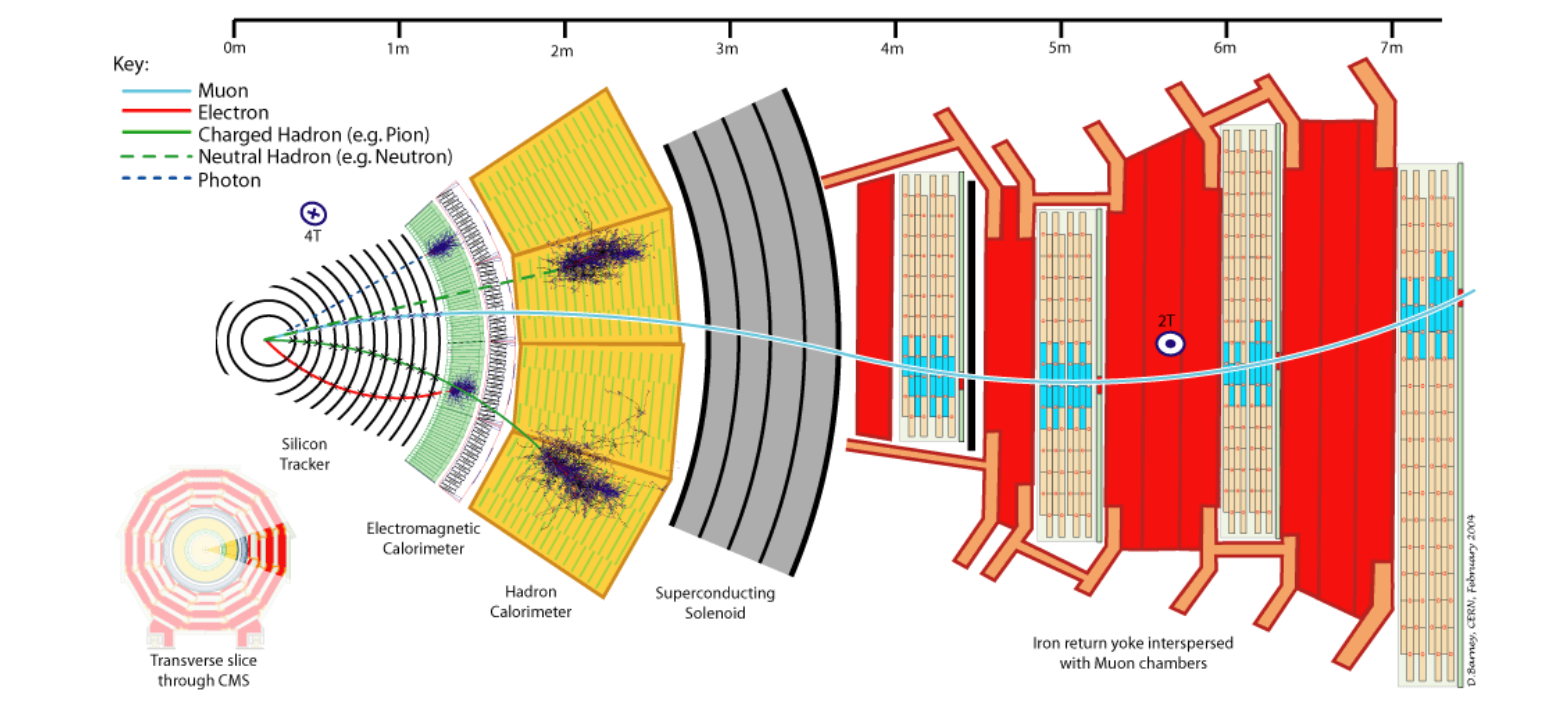
\includegraphics[scale=0.6]{fig/CMSParticleFlow.png}
	\label{fig:CMSParticleFlow}
\end{figure}

For this analysis, we are mostly interested in photons, muons and jets. We are interested in signal events containing two photons and some of our background estimates are derived from jet and muon datasets. 


\subsection{Tracks and Vertices}\label{sec:track_vertex}

Only charged particles can leave discernible tracks in the Silicon Tracker layers due to their interactions with the doped silicon material where impurities in the silicon crystal lattice regions that have excess positive or negative charge. The proper reconstruction of these tracks are fundamental as they are essential for reconstructing the full event topology, as well as the identification of other particles. They contribute towards the subsequent reconstruction of other physics objects in an event. To reconstruct the trajectory of the particles, the tracker hits are fit into the path that likely belong to the same particle track simultaneously discarding irrelevant hits while taking into consideration the hit position uncertainty, the effects of multiple Coulomb scattering as well as energy loss. To reconstruct the tracks, CMS makes use of the Combinatorial Track Finder algorithm (CTF) based on a Kalman filter. The latter is a technique used to recursively estimate quantities such as position, momentum, etc. based on its previous state and updating this prediction using new measurements from the tracker hits. This entire process is described in more detail in in Ref.~\cite{Chatrchyan:2014fea}.


% Charged particles leave tracks as they propagate through the Silicon tracker layers. These tracks are fundamental as they contribute towards the subsequent reconstruction of other physics objects in an event. CMS makes use of the Combinatorial Track Finder algorithm (CTF) based on a Kalman filter to reconstruct tracks by fitting tracker hits taking into account hit position uncertainty and the effects of multiple Coulomb scattering and energy loss. The fit then returns the track information incuding the charge, initial momentum of the particle as well as the impact parameter with respect to the primary vertex. This process is described in more detail in Ref.~\cite{Chatrchyan:2014fea}.

 % By accurately tracing the paths of charged particles, scientists can determine the momenta, energies, and trajectories of these particles. This information is essential for reconstructing the full event topology, including the identification of particles such as electrons, muons, and hadrons, as well as for determining properties such as particle decays and interactions. In essence, the tracks serve as the foundational data upon which further analysis and interpretation of the event rely, making them fundamental to understanding the physics processes occurring within the 
 %detector.

%STUDY NOTES
%  This process involves associating hits that likely belong to the same particle track and discarding irrelevant hits.
% Kalman Filter: The Kalman filter is a mathematical technique used for recursively estimating the state of a dynamic system from a series of noisy measurements. In the context of particle tracking, it's employed to predict the state (position, momentum, etc.) of a particle based on its previous state and to update this prediction using new measurements (tracker hits).
% Hit Position Uncertainty: Each hit has associated uncertainties due to factors like detector resolution and measurement errors. The Kalman filter takes these uncertainties into account when predicting and updating the particle's state, allowing for a more accurate reconstruction of the track.
% Multiple Coulomb Scattering: As charged particles travel through a material, they experience scattering due to interactions with the nuclei of the material. This scattering causes deviations in the particle's trajectory, which need to be considered during track reconstruction. The CTF algorithm incorporates models of multiple Coulomb scattering to better estimate the true path of the particle.
% Energy Loss: Charged particles lose energy as they traverse through a material, primarily through ionization processes. This energy loss can affect the particle's trajectory and momentum, which again must be taken into consideration during track reconstruction. The CTF algorithm incorporates models of energy loss to refine the track reconstruction process.

Since there are approximately $10^11$ protons in each bunch crossing, there are numerous proton-proton collisions occuring simultaneously resulting in pileup interactions, in addition to other interactions coming from particle decays after the hard interaction and interactions with detector materials and cosmic rays. This makes the determination of the primary vertex a challenge. To reconstruct the primary vertex, first, the tracks that are compatible with the LHC beam spot are selected and clustered. This beam spot corresponds to the 3D luminous region where the LHC beams collide. This track clustering algorithm is described in more detail in reference~\cite{Chatrchyan:2014fea}. Multiple primary vertices can be reconstructed in an event due to pileup but the largest summed charge-particle track $\pt^2$, plus some constraints, is chosen as the main primary vertex. Ref.~\cite{CMS:2014pgm} gives more details on the deterministic annealing algorithm used for vertex reconstruction. The paper also achieved a position resolution in each of the 3 spatial dimensions of 10-12~$\mu$m for the reconstructed primary vertices.

For this analysis, the primary interaction vertex associated with the diphoton system is selected using Ref.~\cite{vertex1, vertex2}, which uses a multivariate classifier to enhance the probability of correct vertex assignment. Input variables to the classifier include the $\pt^2$ sum of the charged-particle tracks associated with the vertex, and two variables that quantify the vector and scalar balance of the transverse momentum between the diphoton system and the tracks associated with the vertex. Additionally, if either photon has an associated track originating from a photon conversion to an $e-e+$ pair, the conversion information is used. For signal events above 500~\GeV, a 90\% correct vertex assignment was observed.

% 137 In addition, if either photon has an associated track that has been identified as originating
% 138 from a photon conversion to an electron-positron pair, the conversion information is used. For
% 139 signal events with diphoton invariant masses above 500 GeV, the fraction of events in which
% 140 the interaction vertex is correctly assigned is approximately 90%.


% The primary vertex is determined based on its compatibility with the hard scattering from the pp interactions along the beam line. In each event, there are accompanying secondary vertices resulting from particle decays after the hard interaction. To reconstruct the primary vertex, tracks that are compatible with the LHC beam spot are selected and clustered. The LHC beam spot corresponds to the 3D luminous region where the LHC beams collide. The track clustering algorithm is described more in Ref.~\cite{Chatrchyan:2014fea}. Due to pileup, multiple primary vertices can be reconstructed in an event but the main primary vertex is chosen such that it has the largest summed charge particle track $\pt^2$, with some additional constraints described. Ref.~\cite{CMS:2014pgm} gives more details on the deterministic annealing algorithm used for vertex reconstruction. Their result also achieved a position resolution of 10-12 $\mu$m in each of the three spatial dimensions for the reconstructed primary vertices for interesting \Pp collisions. 

\subsection{Photon and Electron Reconstruction}~\label{sec:PhotonAndElectronRECO}
Photon candidates, being neutral particles, are reconstructed from energy deposits in the ECAL that typically do not have any associated tracks in the tracker. They are evolved from a fixed $5\times5$ matrix of crystals. The "seed crystal" which contains an energy signal greater than all of its immediate neighbors, form as the central piece of a photon cluster~\cite{CMS:2015myp}. The aggregated energy deposits in individual crystals beginning from the seed crystal forms the clusters and superclusters (clusters of clusters)~\cite{Khachatryan:2015iwa} which are compatible with the expected shower shape extending along the azimuthal ($\phi$) direction. This shower shape is similar to electrons but there is a slight difference due to the effect of the magnetic field on the electron trajectory however, the clustering algorithm does not make this distinction. For this reason, the same algorithm for photon reconstruction can be applied to $Z \rightarrow e^+e^-$ events to measure the efficiency of the photon selection criteria and of the photon energy scale and resolution. About 94\% of the photon's energy is deposited in a $3\times3$ group of ECAL crystals and 97\% in $5\times5$ crystals. Any candidate with HCAL energy deposit exceeding $10\%$ of its energy from the ECAL supercluster are rejected. Photon Energy reconstruction includes energy corrections that account for detector effects. For the endcap photons, energy from the ECAL preshower are also added to the photon energy measurement. Pileup contamination and photon shower loss are also accounted for. Photon showers may be lost in the gaps between crystals or ECAL modules. To correct for these losses, the photon efficiency is calculated and the differences between efficiencies in data and simulation are corrected using scale factors (see Sec.~\ref{selection_efficiency}). More details on the full process are found in \cite{Mukherjee:2021wzi}. 

% Photon candidates are reconstructed from energy deposits in the ECAL that typically do not have any associated tracks in the tracker. Individual energy deposits are grouped into superclusters~\cite{Khachatryan:2015iwa} that are compatible with the expected shower shape extending along the azimuthal ($\phi$) direction. This allows for the recovery of the energy deposited by bremsstrahlung and photon conversions. The clustering algorithm does not make any hypothesis as to whether the particle originating from the interaction point is a photon or an electron. Thus the same algorithm used for photon reconstruction can be applied to $Z \rightarrow e^+e^-$ events and these events are used to
% measure the efficiency of the photon selection criteria and of the photon energy scale and resolution. Additionally, these photons should not have any associated HCAL deposit containing more than $10\%$ of its energy from the ECAL supercluster. Photon Energy reconstruction includes energy corrections that account for detector effects. For the endcap photons, energy from the ECAL preshower are also added to the photon energy measurement. Pileup contamination and photon shower loss are also accounted for. Photon showers may be lost in the gaps between crystals or ECAL modules. To correct for these losses, the photon efficiency is calculated and the differences between efficiencies in data and simulation are corrected using scale factors (see Sec.~\ref{selection_efficiency}). More details on the full process are found in \cite{Mukherjee:2021wzi}. 

% Photon and Electron Reconstruction is performed in various steps starting from the clustering of photon energy in the ECAL and track matching. Corrections are applied as well as the energy scale uncertainty.

% Individual particles in the CMS detector are reconstructed using the particle-flow event algorithm~\cite{CMS-PRF-14-001}.
% A more detailed description of photon reconstruction in the CMS detector can be found in Ref.~\cite{Khachatryan:2015iwa}.

% Photons are neutral particles and should leave no track in the inner tracker. However, photons may also convert in the tracker into an electron-positron pair whose paths bend under the influence of the magnetic field. They leave most of their energy deposits in the ECAL. In cases where their trajectories are bent, the energy deposits are extended along the $\phi$ direction. The energy deposits are grouped into so-called ECAL superclusters with transverse energy $E_{T} > 10 GeV$. Details on the procedures on how these superclusters are formed are found in \cite{PhotonReconstruction_2015}. Additionally, these photons should not have any associated HCAL deposit containing more than $10\%$ of its energy from the ECAL supercluster. 
% Photon Energy reconstruction includes energy corrections that account for detector effects. For the endcap photons, energy from the ECAL preshower are also added to the photon energy measurement. Pileup contamination and photon shower loss are also accounted for. Photon showers are lost in the gaps between crystals or ECAL modules. To correct for these losses, the photon \textbf{efficiency} is calculated and the differences between efficiencies data and simulation are corrected using \textbf{scale factors}. More details on the full process are found in \cite{PhotonAndElectronReco}

% Electrons are reconstructed by associating a clus-
% ter in the ECAL with a track in the tracker. The
% clusters are reconstructed by summing up the en-
% ergy deposits in crystals surrounding the “seed” crys-
% tal, which is locally the crystal with largest energy
% deposit. The summing algorithm incorporates en-
% ergy deposits arising from bremsstrahlung emissions
% in the tracker. Energy clusters in the ECAL are
% matched to hits in the inner tracker, which are then
% used to seed tracks in the rest of the tracking detec-
% tor. A dedicated electron track reconstruction algo-
% rithm, known as Gaussian Sum Filter (GSF) algo-
% rithm, accounts for bremsstrahlung emission before
% the calorimeter. The resulting cluster–track matched
% objects form the final electron candidates. 

% The effi-
% ciency for electron reconstruction is measured with
% the tag-and-probe method [3, 4] by using Z → ee
% events. A tag electron is established by applying
% tight cuts to one electron candidate; the other can-
% didate is used as a probe. A large sample of high-
% purity probes is obtained by requiring that the tag-
% and-probe pair has an invariant mass consistent with
% the Z-boson mass. All efficiencies and scale factors
% described in this article, including trigger efficiency,
% the GSF track reconstruction efficiency in the sili-
% con tracker, electron and photon identification effi-

Electrons being charged particles are reconstructed by associating an ECAL cluster with a track in the tracker. The ECAL clusters are reconstructed by summing up the energy deposits in the crystals around the ``seed" crystal which has largest energy deposit. These clusters are matched to hits in the inner tracker using the Gaussian sum filter (GSF) algorithm. Both the summing and the GSF algorithms take into account the energy deposits arising from the bremsstrahlung emissions in the tracker~\cite{Mukherjee:2021wzi}.

% Electrons being charged particles should leave tracks in the tracker. To reconstruct these objects, the tracks are matched to an ECAL supercluster.  using the same method for photons that convert into electron-positron pairs in the tracker. To date, the standard track reconstruction uses a Gaussian sum filter (GSF) to fit the tracker hits. The GSF also takes account secondary tracks coming from emitted bremsstrahlung photons. More details on the procedure are found in \cite{CMS:2015xaf}.

%% Khachatryan:2015iwa is the same as CMS:EGM-14-001 cited in Detector section
% \FIXME{}
\subsection{Muon Reconstruction}

Muon candidates are reconstructed from information from the dedicated muon system and inner tracker. These particles ionize the gas in the chambers and leave hits whose precise locations are determined more accurately. The hits in DT and the CSC are used to reconstruct track segments in the muon system. The requirements for these hits include the following: an angular cone of $\Delta R < 0.3$, and the summed $p_{T}$ of any additional tracks and calorimeter deposits should not exceed 10$\%$ of the muon track's $p_{T}$. These reconstructed muon tracks must also be compatible with a track in the inner tracker. A best track fit between the inner and outer track including information from the RPCs is employed~\cite{CMS:2018rym}. 


% The presence of reconstructed tracks from the outer tracking muon system must satisfy compatibility requirements with a track in the inner tracker. The track segments in the muon system are generated by requiring a certain number of hits in the layers within a single DT or CSC chamber. Within an angular cone of $\Delta R < 0.3$, the summed $p_{T}$ of any additional tracks and calorimeter deposits should not exceed 10$\%$ of the muon track's $p_{T}$. For $p_{T} < 200$ GeV, the muon $p_{T}$ and direction are based on the associated inner track's momentum and direction. Above that, they are based on the best track fit between the inner and outer track, with the information from the RPCs included. More details on the algorithm used are found in Ref.~\cite{CMS:2018rym} 

\subsection{Jets Reconstruction}

Jets are collimated spray of hadrons that appear as a cluster of energy in the ECAL and HCAL subdetectors. These candidates are only reconstructed after isolated photon, electron and muon candidates have already been identified from the pool of particle flow candidates. There are multiple algorithms used to reconstruct jets. The anti-$k_{t}$ algorithm~\cite{antikt_algorithm} is a typical method used and is suitable for reconstructing jets with well-defined boundaries. These candidates are further classfied into neutral (e.g. $K^{0}$), charged hadrons (e.g. $\pi^{\pm}$, $K^{\pm}$, protons) and non-isolated photons($\pi^{0}$). Non-isolated photons have ECAL clusters that are not linked to any track. Neutral hadrons are also not linked to any track but have energy clusters in the HCAL. Reconstructed tracks matching to ECAL and or HCAL clusters form charged hadrons. Their energy deposits are corrected to account for the nonlinear response of the calorimeters. For $|\eta| > 2.5$, neutral hadrons cannot be distinguished from charged hadrons since that range is beyond the tracker acceptance.  For non-isolated photons or neutral hadrons, their energies are determined by the corrected ECAL or HCAL cluster energy or the combined cluster energy of ECAL and HCAL if $|\eta| > 2.5$. Charged hadron energies are derived from whichever is the larger value between the calorimeter cluster energies or the sum of the matched track momenta \cite{Strologas:2287326}. 




% Jets are reconstructed from what is left from the pool of PF candidates after isolated photon, electron, and muon candidates have been reconstructed. The anti-$k_{t}$ algorithm \cite{antikt_algorithm} with a radius parameter $R=0.5$. These candidates are further classified into charged hadrons (e.g. $\pi^{\pm}$, $K^{\pm}$, protons), neutral hadrons (e.g. $K^{0}$) and non-isolated photons ($\pi^{0}$). 
% STUDY notes
% Reconstruction of jets and missing transverse momentum at the CMS experiment: Run 2 and perspective for
% Run 3 Andrea Malara
% 1. Introduction
% In the hadronic environment at the LHC, many quarks and gluons are produced, which, due
% to QCD confinement, create a collimated spray of hadrons, which appear as a cluster of energy
% deposited in a localised area of the detector, called a jet. Precise calibration of both the energy
% scale and resolution of jets plays a crucial role across the whole physics programme at the CMS
% experiment. Similarly, an accurate estimation of the missing transverse momentum (��miss
% T ) is of
% crucial importance, for example, in standard model measurements involving the invisible decay
% products of the top quark, �� lepton and the W, Z and Higgs bosons, as well as in beyond the standard
% model searches targeting new weakly interacting neutral particles.

% The jet performance is quantified with a sample of QCD multijet events. Jets are reconstructed
% with the anti-kT algorithm (radius parameter R = 0.4) [43, 44]. The algorithm clusters either
% all particles reconstructed by the PF algorithm (PF jets), or the sum of the ECAL and HCAL
% energies deposited in the calorimeter towers2 (Calo jets), or all stable particles produced by the
% event generator excluding neutrinos (Ref jets). Particle-flow jets are studied down to a pT of 15 GeV,
% while Calo jets with a pT lower than 20 GeV are deemed unreliable and are rejected.

\section{Event Selection}~\label{sec:EventSelection}
This analysis selects events containing two high-energy, prompt photons. To select these events, an online trigger selection, and further offline selection and photon identification criteria are imposed. These further selections ensure that the  photons are well-measured and isolated from other particles in the event, help reduce background from other processes and thereby increase the sensitivity of this analysis. 

\subsection{Trigger Selection}~\label{sec:TriggerSelection}

Events for this analysis are selected online by an online trigger (HLT) containing at least two reconstructed photon candidates, each with transverse momentum $p_{T} > 60 (70)$~GeV, for the 2016 (2017/2018). We refer to these as the Double Photon Triggers. The two leading photons in $\pt$ are chosen in events with more than two photon candidates. The trigger photon candidates are also required to have a ratio of hadronic/electromagnetic energy of less than 0.15. 


% Events for this analysis are required to pass an online high-level trigger (HLT) selection containing two reconstructed photon candidates each with a transverse momentum $p_{T} > 60 (70)$~GeV in the range $|\eta| < 3.0$ for 2016 (2017/2018). Each photon candidate must also have a ratio of the hadronic to the electromagnetic energy (H/E) $<$ 0.15. The electromagnetic energy here is defined as the corrected supercluster energy while the hadronic energy is the total HCAL energy within a cone of $\Delta R <$  0.15 from the supercluster position. This ratio is also the amount of the HCAL energy in the tower directly behind the photon seed crystal. 

%From paper
% Events are selected online by a trigger that requires at least two reconstructed photon candi-
% 111 dates, each with transverse momentum pT > 60 (70) GeV, for the 2016 (2017–2018) data sets.
% 112 In events with more than two photon candidates, the two photons leading in pT are chosen.
% 113 The trigger photon candidates are required to have a ratio of hadronic/electromagnetic energy
% 114 of less than 0.15. With these selections, the trigger efficiency is consistent with 100% for two
% 115 offline photons with pT > 125 GeV.

% Two diphoton event categories are considered in this analysis: the first category is where both
% 117 photons are reconstructed in the fiducial region of the EB with |η| < 1.44 (denoted EBEB),
% 118 while the second category consists of events with one photon in the EB and the other photon
% 119 in the fiducial region of the EE, 1.57 < |η| < 2.5 (EBEE). Photons in the overlap region be-
% 120 tween 1.44 < |η| < 1.57 have low reconstruction efficiency and hence are not used. The EBEE
% 121 category typically provides an approximately 10% increase to the signal sensitivity, whereas
% 122 events where both photons are in the EE are not considered because this category is dominated
% 123 by SM backgrounds and has negligible sensitivity to the target signal models. The minimum
% 124 reconstructed invariant mass of the diphoton system is required to be mγγ > 500 GeV. Photon
% 125 pairs must additionally satisfy ∆Rγγ > 0.45 to be consistent with the calculation used for SM
% 126 diphoton production described in Section 5.

To quantify the efficiency of the Double Photon triggers, we use a reference for normalization. This reference trigger selects events that contains two photons each with transverse momentum greater than 33 GeV and satisfies the Calorimeter Identification (CaloId) criteria. The efficiency is primarily a function of the $p_{T}$ of the second-leading photon, the photon which has the second highest $p_{T}$ among the collection of photons. The results are shown in Figure~\ref{fig:trigger_efficiency}. The precise form of the fit is irrelevant as the efficiency plateaus well before the offline cut value. This procedure only probes the turn-on of the $p_{T}$ leg \cite{ref:AN2016_167} have shown that there is no additional source of efficiency and this study serves as a cross-check. An additional backup trigger was also used to mitigate potential efficiency losses at high diphoton invariant masses. We calculated an additional 0.2$\%$ yield over the full analysis region with several thousand events, without viewing any distributions to avoid bias during the blinded phase of the analysis. The trigger efficiency is fully efficient at $p_T > 125$ GeV, which is the photon $p_{T}$ selection used in this analysis. For details on the exact trigger path names see Appendix~\ref{ch:appendix_datasets_triggerpaths}.

% These selection details are contained in the trigger code \texttt{HLT\_DoublePhoton60} or \texttt{HLT\_DoublePhoton70} for 2016 and 2017/2018 data respectively.

% Events for this analysis are required to pass a high-level trigger selection containing two reconstructed photon candidates in the range |eta|< 3, above a certain threshold in transvserse momentum. That threshold value was 60 GeV for the 2016 dataset and 70 GeV for the 2017/18 datasets. Each photon candidate must have  …had/em… etc…
% At the Level1 trigger stage, the events were required to pass  …. [here describe the triggers without using the trigger names. You can see what is written in our journal papers for inspiration]
% To quantify the efficiency of the HLT triggers, we consider a reference trigger with a lower pT threshold and  looser photon identification requirements …

% Events containing two prompt photon events are selected online with \texttt{HLT\_DoublePhoton60} or \texttt{HLT\_DoublePhoton70} trigger paths for 2016 and 2017/2018 data respectively. These two triggers require at least two reconstructed photon candidates with a transverse momentum $p_{T} > 60 (70)$~GeV across the range $|\eta| < 3.0$. At this level, the primary selection requires that each photon candidate must have a ratio of the hadronic to the electromagnetic energy (H/E) $<$ 0.15. The electromagnetic energy here is defined as the corrected supercluster energy while the hadronic energy is the total HCAL energy within a cone of $\Delta R <$  0.15 from the supercluster position. This ratio is also the amount of the HCAL energy in the tower directly behind the photon seed crystal. 

% To quantify the efficiency of the \texttt{HLT\_DoublePhoton60/70} triggers, we used the reference trigger \texttt{HLT\_DoublePhoton33\_CaloIdL} for normalization. The \texttt{HLT\_DoublePhoton33\_CaloIdL} trigger selects events that contain two photons, each with transverse momentum greater than 33 GeV and satisfying the Calorimeter Identification (CaloId) criteria.

% The efficiency is primarily a function of the $p_{T}$ of the second-leading photon, the photon which has the second highest $p_{T}$ among the collection of photons. The results are shown in Figure~\ref{fig:trigger_efficiency}. This procedure only probes the turn-on of the $p_{T}$ leg \cite{ref:AN2016_167} have shown that there is no additional source of efficiency and this study serves as a cross-check. 



% generated by Tools/bin/efficiency.cc
\begin{figure}[htbp!]
\caption{Efficiency of the Double Photon triggers (measured with reference trigger as a function of the \pt of the second-leading photon in 2016 (left), 2017 (center) and 2018 (right) data.}
\begin{center}
%\includegraphics[angle=0,width=0.4\textwidth]{figures/eff2015.pdf}
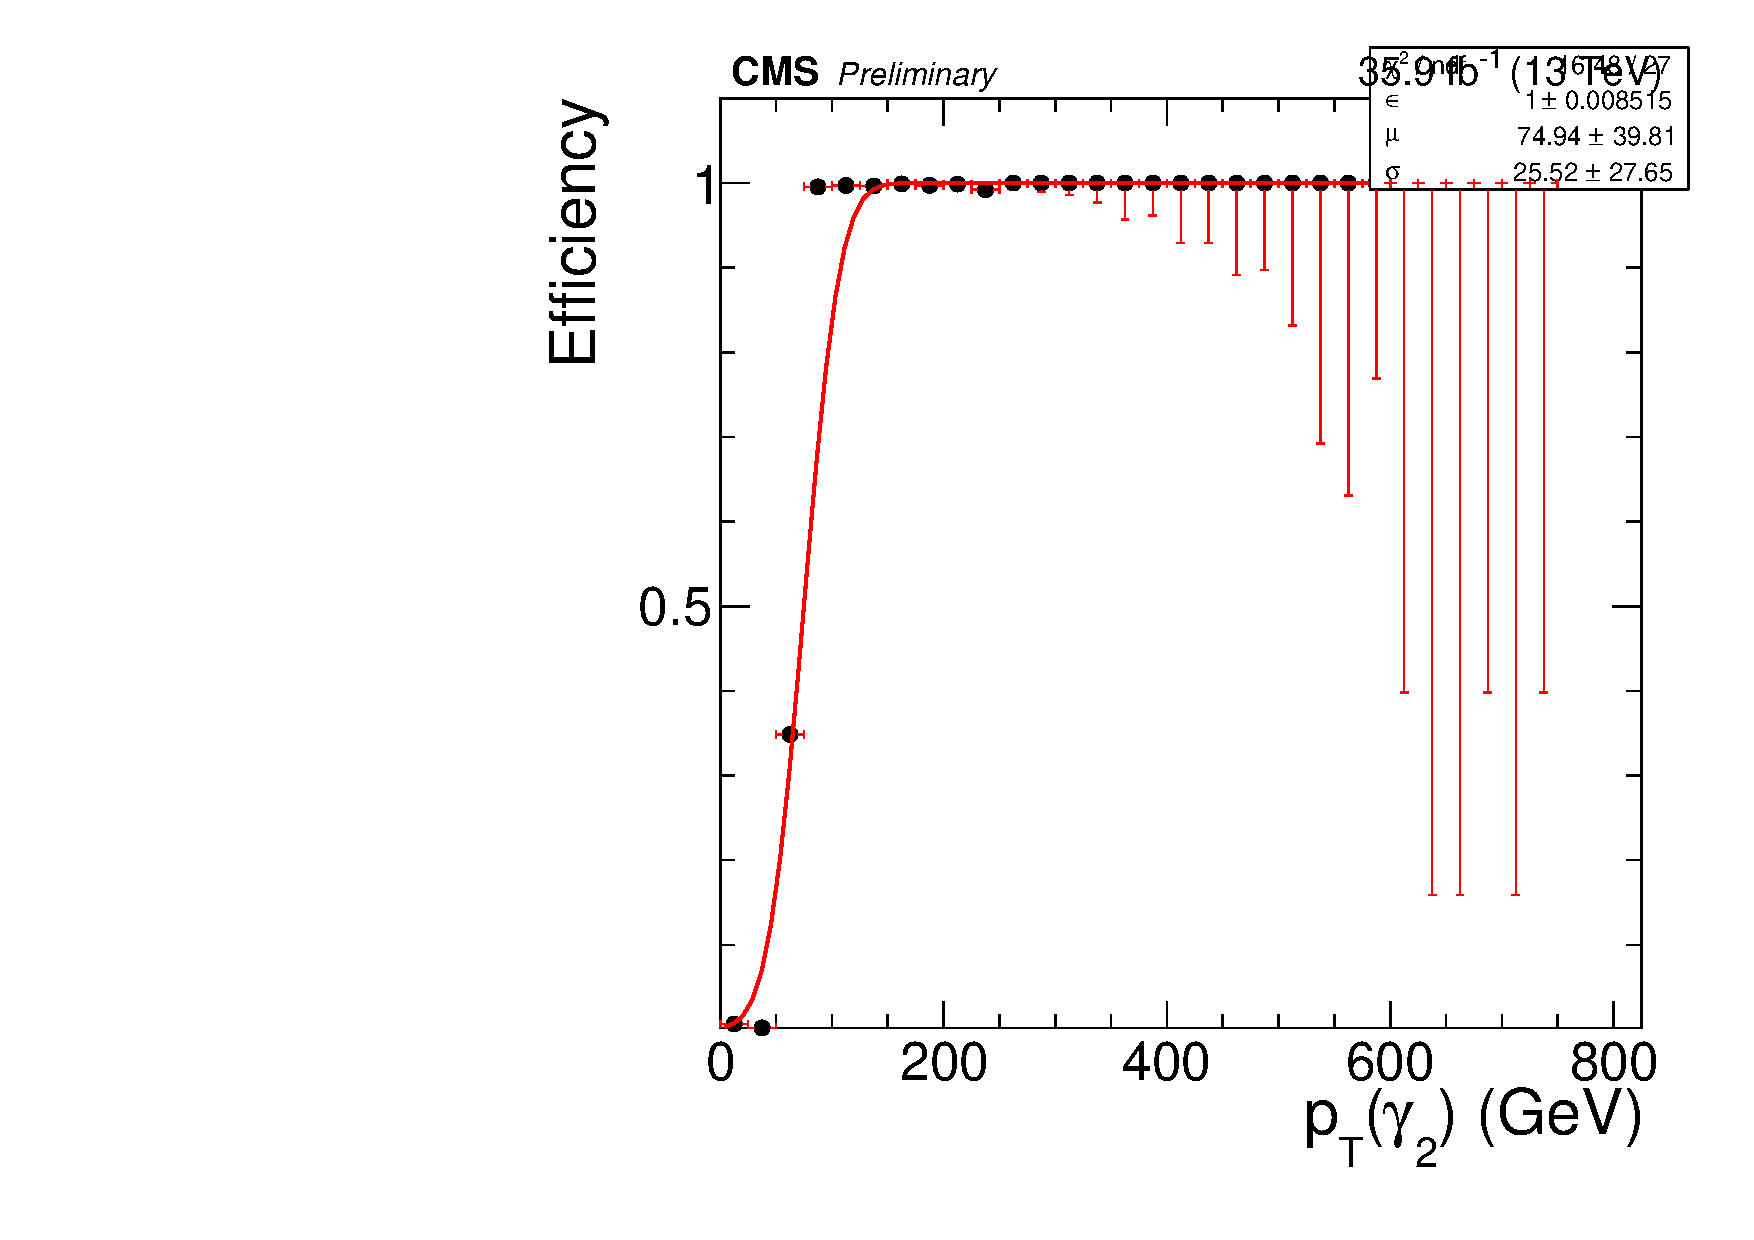
\includegraphics[angle=0,width=0.3\textwidth]{fig/eff_2016_Photon2_pt.pdf}
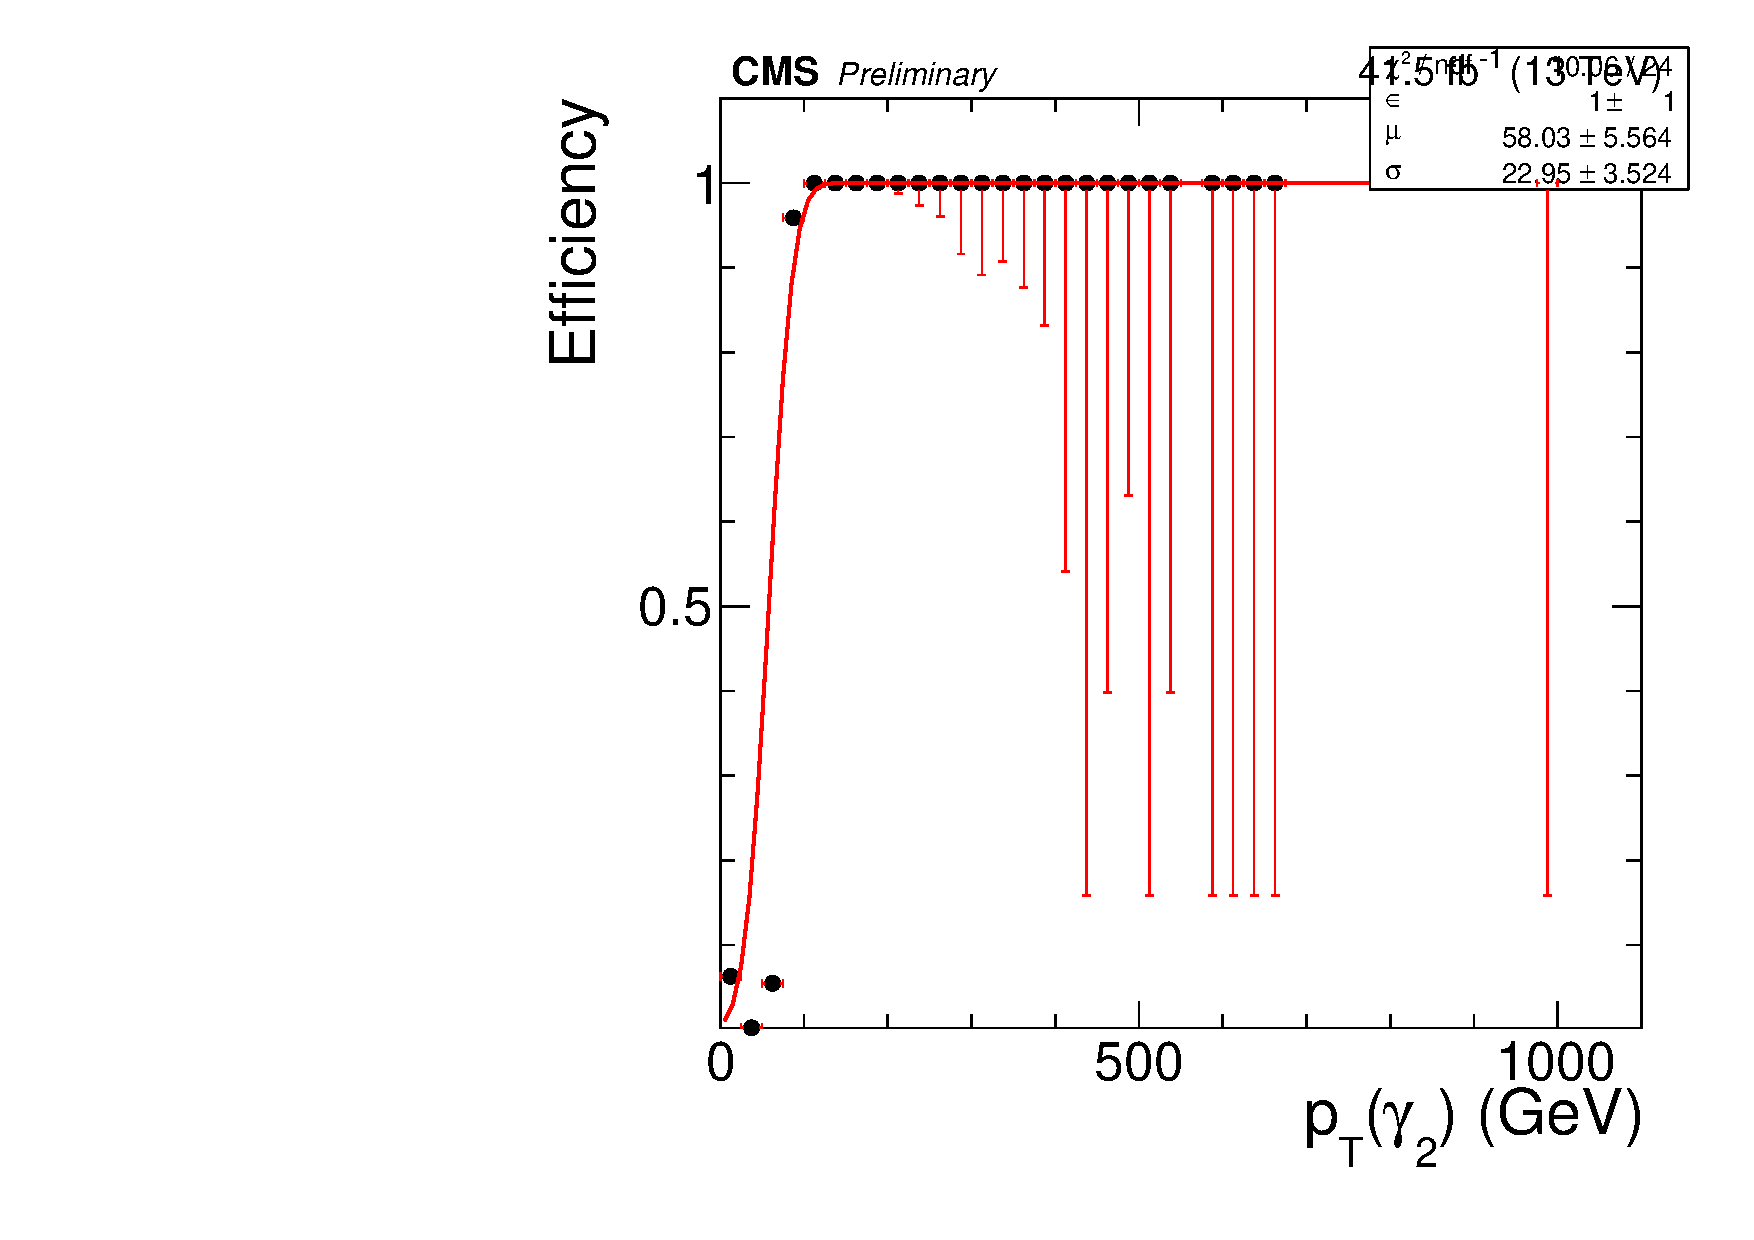
\includegraphics[angle=0,width=0.3\textwidth]{fig/eff_2017_Photon2_pt.pdf}
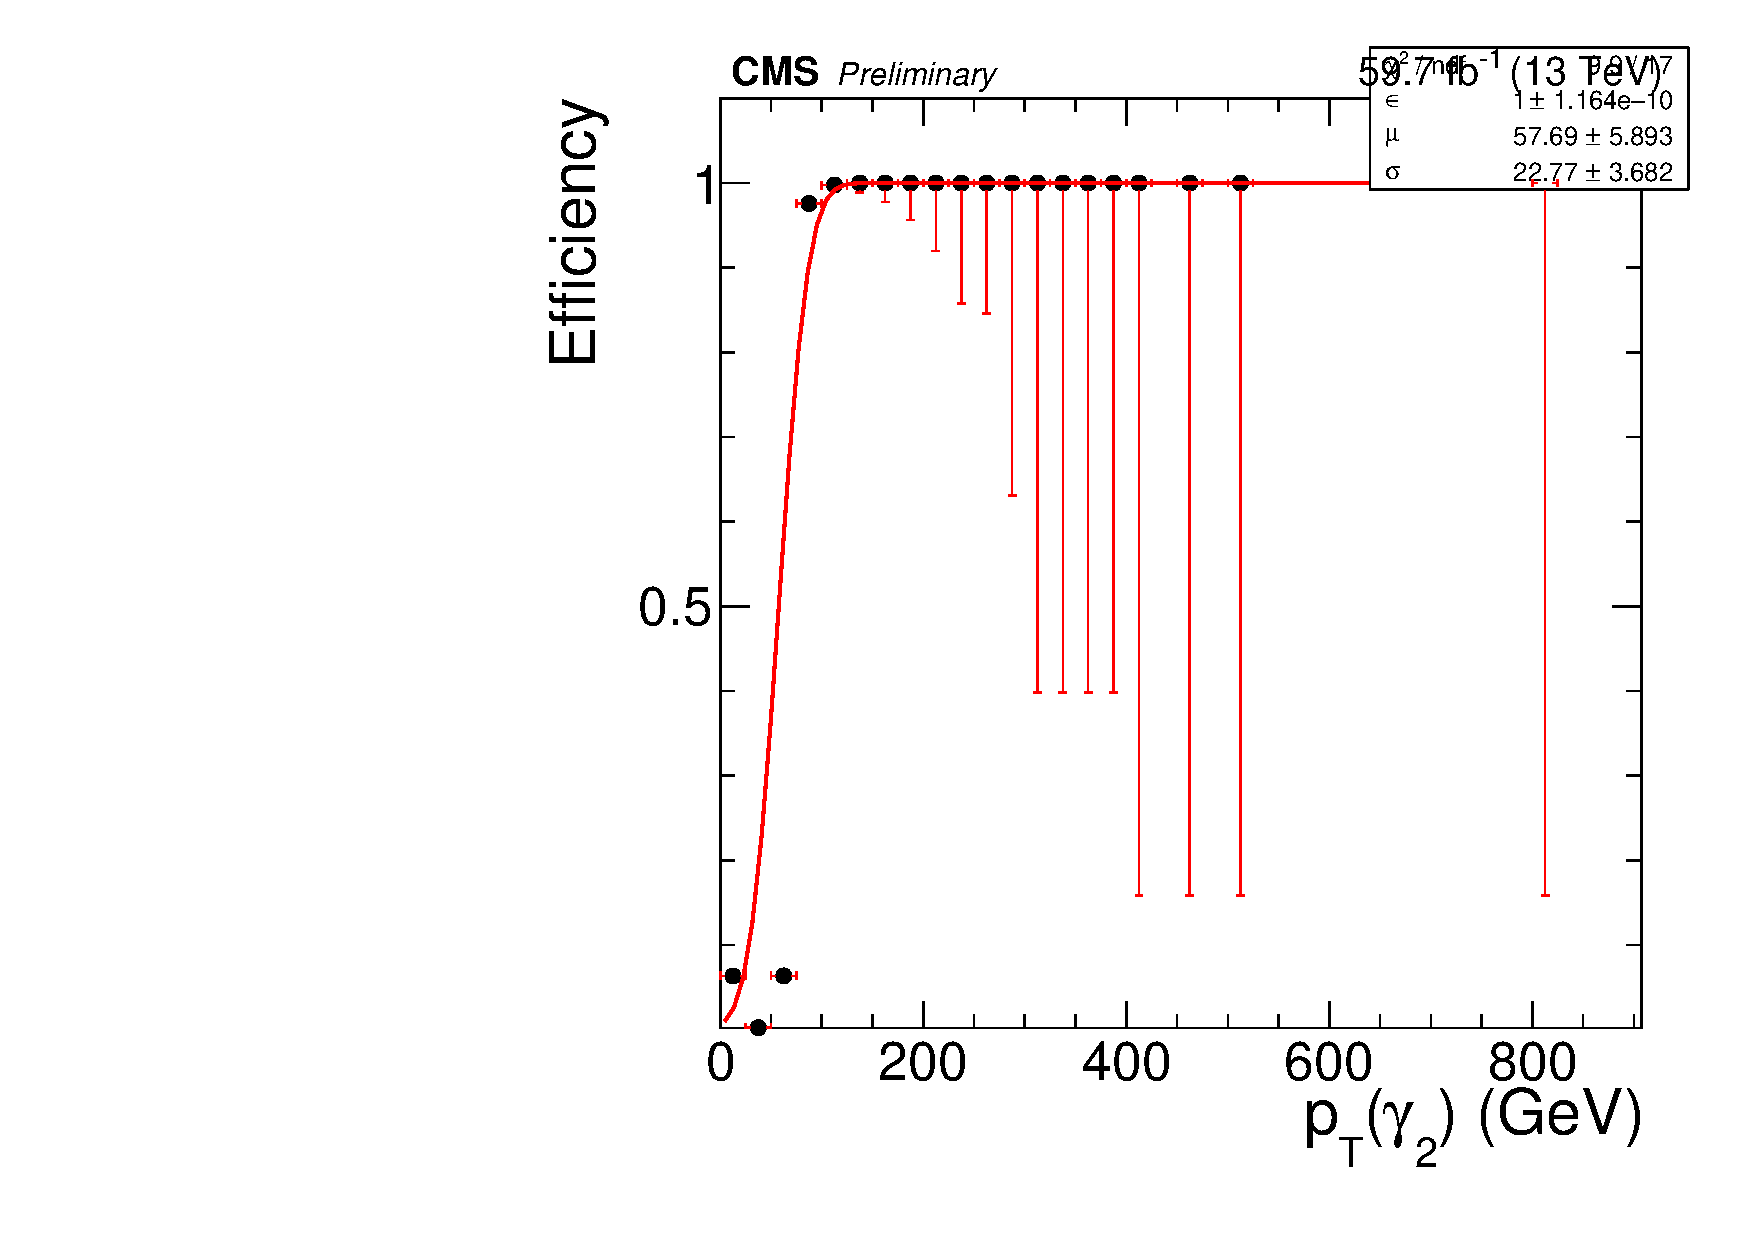
\includegraphics[angle=0,width=0.3\textwidth]{fig/eff_2018_Photon2_pt.pdf}
\end{center}
\label{fig:trigger_efficiency}
\end{figure}


\subsection{Photon Identification}~\label{subsec:photonID}
The reconstructed photon candidates passing the trigger selection must pass additional identification criteria to supress background events coming from misidentified jets and electrons while maintaining high efficiency. These criteria are based on observables sensitive to the electromagnetic shower shape, shower containment within ECAL and any extra activity surrounding the shower. The electromagnetic shower is  measured using \sieie. The \sieie variable~\cite{Khachatryan:2015iwa}, is the spatial second-order moment of the photon candidate with coordinates $(\eta_\gamma,\,\phi_\gamma)$. It is defined mathematically as follows:

\begin{equation}
    \sigma_{i\eta_{i} i\eta} = \sqrt{\frac{\sum_i w_i (\eta - \Bar{\eta})^2}{\sum_i w_i}}
\end{equation}

where $w_i = max(0.0, 4.7 + ln E_{i}/E_{5x5})$, $\eta_{i}$ is the coordinate of crystal $i$ in the $5 \times 5$ array, $\Bar{\eta}$ is the average supercluster position in $\eta$, $i$ runs over a $5\times 5$ matrix of crystals centered on the crystal with maximum energy deposit and the sums are taken over all the crystals in the matrix. This variable is a measure of the spread of the energy distribution within the crystal matrix, along the $\eta$ direction of the detector. It is a useful quantity for identifying electromagnetic showers initiated by electrons or photons, which typically have a narrow, localized distribution of energy, in contrast to showers initiated by hadrons, which are broader and more diffuse. Prompt photons have smaller values of \sieie corresponding to narrower showers. The variable $\sigma_{i\phi_{i} i\phi}$ is defined analogously and together with \sieie they form a covariance matrix which describes the spatial extension of the electromagnetic showers in the $(\eta, \phi)$ space. Additionally, a selection on the shower shape variable $R_{9} < 0.8$ is imposed to reduce the contribution of jets that fake photons. $R_{9}$ is defined as the ratio of the energy deposited in a $3\times 3$ array of crystals centered around the most energetic crystal in the supercluster, to the total energy deposited in the supercluster. It is a measure of the degree of lateral containment of the shower. Values closer to 1 indicate a more compact shower and values closer to 0 indicate a more spread-out shower. 

\begin{figure}[!htbp]
	\centering
     \caption{Prompt photons (REAL) and Fake Photons are shown on top and bottom. The figures on the left show the \sieie distributions for real and fake. On the right, a representative illustration of a prompt (fake) photon energy deposit in a $5 \times 5$ array of crystals is shown on top (bottom).}
	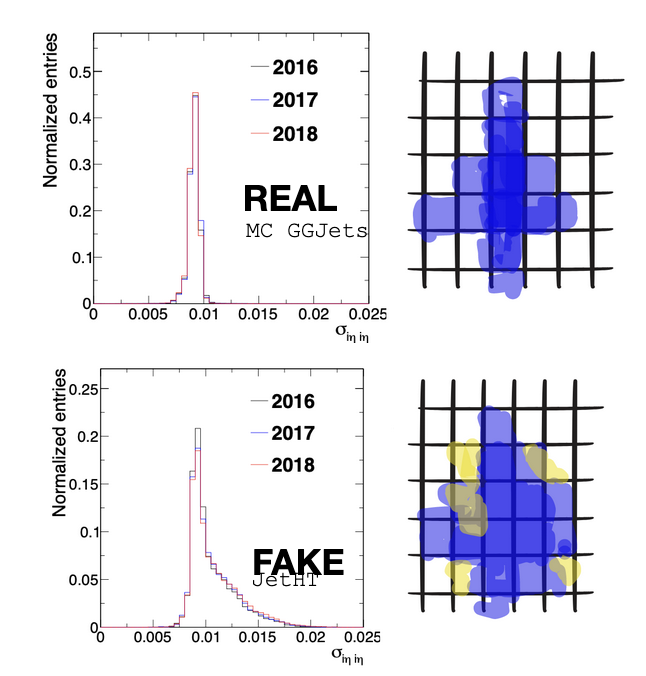
\includegraphics[scale=0.9]{fig/PromptPhotonsVsFakes.png}
	\label{fig:PromptPhotonsVsFakes}
\end{figure}

Photons in the event should also be well-isolated hence isolation variables which describes the degree to which a photon is isolated from other particles in an event are also used in the identification criteria. These variables are based on the total transverse momentum of the particle candidates with $(\eta,\,\phi)$ coordinates that are reconstructed within a cone size of $\Delta R < 0.3$ around the photon candidate with coordinates $(\eta_\gamma,\,\phi_\gamma)$. Here, $\Delta R = \sqrt{(\eta - \eta_\gamma)^2 +(\phi-\phi_\gamma)^2}$. Charged hadrons ($Iso_{Ch}$) and Photon candidates ($Iso_{\gamma}$) are defined separately. It was found that prompt photons are well-isolated for both variables. The photon isolation variable is also found to be dependent on photon transverse momentum and pileup. To mitigate the effect, we define a corrected photon isolation variable that has been pileup subtracted with $p_{T}$ dependence as follows, 
% Isolation variables are based on the total transverse momentum of the particle candidates with $(\eta,\,\phi)$ reconstructed within a cone of size $\Delta R < 0.3$ around the photon candidate with coordinates $(\eta_\gamma,\,\phi_\gamma)$, where $\Delta R = \sqrt{(\eta - \eta_\gamma)^2 +(\phi-\phi_\gamma)^2}$. Separate isolation variables are defined for charged hadron ($Iso_{Ch}$) and photon candidates ($Iso_{\gamma}$). Prompt photons are well-isolated for both variables. $Iso_{\gamma}$ isolation variable is also found to be sensitive to photon $p_{T}$, and pileup. We then use a corrected photon isolation variable that has been pileup subtracted with $p_{T}$ dependence removed according to:

\begin{equation}
 \corphoiso = \alpha + Iso_{\gamma} - \rho A + \kappa p_{T}  
\end{equation}

where $\kappa$ is a $p_{T}$ coefficient, $\rho$ is the average pileup $p_{T}$ flow density per unit area in the event obtained from the jet area method~\cite{Cacciari:2008gp, Cacciari:2011ma}, $A$ is the effective area of the isolation region multiplied by an $\eta$-dependent correction factor, and $\alpha$ is a constant measured from experiment chosen to make the \corphoiso peak near zero. More details on the pileup removal are found in Ref.~\cite{CMS:2020ebo}.

% “Saturated crystals” -> it is not the *crystal* that saturates, it is the electronic readout of the energy that reaches a maximum, because there are only a certain number of bits to encode the readout, so at some point, all energies above a certain value will give the same max readout value.
 
The cuts on these variables are summarized in Table~\ref{table:highptid}. In the case of saturated crystals, a situation where the energy deposited by a particle exceeds the crystal's capacity to accurately measure that energy, a different \sieie cut is used to recover efficiency. Note that it is not the crystal itself that gets saturated but the electronic readout of the energy reaches a maximum. Since only a certain number of bits encode the readout, energies above maximum are given the same readout value. ECAL readout electronics saturate at around 1.7 (3.0) TeV in the barrel (endcaps). Objects with very high energy electromagnetic showers which deposit energy in a single crystal must take into account this saturation \cite{saturation_readout, Clerbaux:2006kp}. For our purposes, this impact is negligible. We counted saturated photons passing a preselection of $p_{T} > 125$ GeV and $M_{\gamma\gamma} > 500\GeV$ in the full 2016-2018 dataset. Only one saturated photon was observed in both the barrel region and one in the endcap. This counting allows to avoid simply relying entirely on simulation to validate the assumption that saturated photons are negligible. We did not check any other details of these photons or whether they passed the final selection, to avoid bias during the blinded phase of the analysis. 

Finally, we apply the energy scale and smearing corrections recommended by the CMS Electron/Photon Physics Object Working Group~\cite{EGM_twiki}. These residual corrections scale the data to the MC and smear the MC to the resolution matched in the data. The photon energy scale correction is a multiplicative correction applied to the photon energy, which ensures that the energy measured in the detector corresponds to the true energy of the photon. The correction is typically determined using a combination of simulation and data-driven techniques, such as measuring the energy of photons produced in the decay of the Z boson~\ref{selection_efficiency}. The correction is typically a function of the photon energy and other variables, such as the position of the photon in the detector. The photon energy resolution, or smearing, correction is a Gaussian smearing applied to the photon energy to account for the detector resolution. The smearing is typically determined from simulation studies and depends on the photon energy and other variables, such as the angle of the photon with respect to the beamline. The energy resolution is often parameterized as a function of the photon energy and the pseudorapidity of the photon.

The Conversion-safe electron veto is designed as a variable that rejects direct electrons and not electrons that might come from photon conversions. This veto requires that a photon cluster in the ECAL is not matched to a reconstructed conversion vertex, and a hit in the inner layer of the pixel detector associated with a charged-particle track indicating a direct and real electron~\cite{CMS:2015myp}. 

% The photon identification prescriptions discussed in this paper use the “conversion-safe elec-
% tron veto” to reject electrons. This veto requires that there be no charged-particle track with a
% hit in the inner layer of the pixel detector not matched to a reconstructed conversion vertex,
% pointing to the photon cluster in the ECAL. The “hit in the inner layer” is computed as a hit in
% the first layer where a hit is possible, accounting for the small number of inoperative sensors,
% and for geometrical configurations where a track can pass between the first layer of sensors
% without leaving a hit. The photon inefficiency is thus reduced, almost entirely, to that resulting
% from photons converting in the beam pipe.

% Conversions can occur when the photons hit materials before they reach the ECAL crystals. The photon energy supercluster is checked for whether it is shared by an electron candidate. If it is, additional checks on missing on the existence hits are required. If none exis

% We predicted 0.22 (0.06) \FIXME{Where was this information obtained?} events with saturated photons in the full 2016-2018 dataset in the barrel-barrel (barrel-endcap) signal region.

%-----------------------------------------------------------------------------
\begin{table}[h]{ \caption{Selection details for the high-\pt photon ID v2. Numbers in $[~]$ are used if the crystal is saturated.}\label{table:highptid}\begin{center}\begin{tabular}{c|cccccc}\hline
Photon  & \chiso &\corphoiso& H/E        &$R_{9}$  & \sieie  &Conversion-safe            \\
category& (GeV)  & (GeV)    & (tower-based)&         & &electron veto              \\ \hline
EB               & $<$5     & $<$2.75      & $<$0.05 & $< 0.8$ & $<$0.0105 [0.0112]&applied \\
EE               & $<$5     & $<$2.0       & $<$0.05 & $< 0.8$ & $<$0.0280 [0.0300]&applied \\ \hline
\end{tabular}\end{center} }\end{table}
%-----------------------------------------------------------------------------

\subsection{Offline Event Selection}~\label{sec:OfflineEvtSel}
Events are selected which contain two photons passing the above ID requirements and having $\pt > 125\GeV$. This \pt selection is set above the trigger threshold described in Sec.~\ref{sec:TriggerSelection} to ensure uniform efficiency. Each of the diphoton candidate is assigned a primary vertex from which the photon candidate's kinematic properites like invariant mass, $\mgg$ are computed.
% We select events which contain at least two photons passing the above ID requirements~\ref{table:highptid} with each photon having $p_{T} > 125$ \GeV. This \pt selection is set above the trigger threshold to ensure uniform efficiency. 
% Each diphoton candidate is assigned a primary vertex and the photon candidate's kinematic properties are computed. The primary $\Pp\Pp$ interaction vertex is the candidate vertex with the largest value of summed physics-object $\pt^2$. These physics objects are the jets which are clustered using the jet finding algorithm~\cite{Cacciari:2008gp,Cacciari:2011ma} with the tracks assigned to candidate vertices as inputs, and the associated missing transverse momentum, taken as the negative vector sum of the \pt of those jets. 
We consider two diphoton event categories: the first category (denoted EBEB) is where both photons are reconstructed in the fiducial region of the ECAL barrel (EB) with $|\eta| < 1.4442$, while the second category (denoted by EBEE) consists of events with one photon in the EB and the other photon in the fiducial region of the EE, $1.566 < |\eta| < 2.5$. Photons landing in the overlapping region between $1.44 < |\eta| < 1.57$ have low reconstruction efficiency and are excluded in the analysis. Events where both photons are in the EE are also not considered since this category is dominated by SM backgrounds and has negligible sensitivity to the target signal models. The EBEE category on the other hand, contributes an additional 10\% sensitivity to the EBEB category. Additionaly, photon pairs must angularly separated by $\Delta R> 0.45$ to be consistent with the MC SM diphoton production calculations to be described in the next chapter.


% Events are also required to have one photon in the ECAL barrel (EB) and the other landing either in the barrel (EB) or endcap (EE). EB covers the range $|\eta| < 1.4442$ while the endcap has $1.566 < |\eta| < 2.5$. Events with both photon candidates in the EEs are rejected. From these we consider two signal regions, (1) EBEB - where two photons are found both in the barrel, and (2) EBEE - where one photon is in the barrel and the other is in the endcap. The diphoton invariant mass must satisfy a minimum requirement of $\mgg>600$~\GeV in both EBEB and EBEE categories. This threshold avoids sculpting of the distribution while maintaining full efficiency in each region. 

% Photon pairs must additionally satisfy $\Delta R> 0.45$, to be consistent with the background calculation for SM diphoton production, as described in the next chapter.

% The combined acceptance and efficiency of this selection for signal events is shown in Section~\ref{sec:signal}. It is found to be roughly 60\% for the highest-mass signal models studied her

\subsection{Photon ID Efficiency and Scale Factors}~\label{selection_efficiency}
The efficiency of the high-$p_{T}$ photon ID was measured using the tag-and-probe (TnP) technique~\cite{generic_TnP}. It is a technique used to get a high purity set of physical objects from known resonances such as $J/\psi$ and Z. Due to the similarity between the photon and electron IDs, the $Z \to e^{+}e^{-}$ channel is chosen to compute the photon ID scale factors which are corrections to the efficiency difference between data and MC. The determination of these corrections is a critical ingredient in any physics analysis as it accounts for particles missed by reconstructions and any inefficiencies in the algorithms used. 

In the generic tag-and-probe technique, one of the electrons in the $Z \to e^{+}e^{-}$ resonance decay, labeled as tag, is required to pass a tight identification criteria while the probe passes a looser identification. For this analysis, we define the efficiency as the ratio of signal yield of the passing probe and the sum of the signal yields of the passing and failing probe:

\begin{equation} \label{eq:efficiency}
  \text{Efficiency} = \frac{\text{Signal Yield}_{\text{passing probe}}}{\text{Signal Yield}_{\text{passing probe}} + \text{Signal Yield}_{\text{failing probe}}}.
\end{equation}
These signal yields were obtained by fitting the passing and failing probe distributions for each $\eta-\pt$ bins with the signal + background model. Representative fitting results are shown in Figure~\ref{fig:Sysbkg}. The scale factors obtained from the ratio between the Data and MC efficiencies for different years are shown in Figure~\ref{fig:SFvsPt}. They are calculated by dividing the efficiency in data and the MC in $\eta-\pt$ bins as shown in this equation. 

\begin{equation} \label{eq:SF}
  \text{Scale Factor}(\eta,p_{T}) = \frac{\text{Efficiency}_{\text{Data}}(\eta,p_{T})}{\text{Efficiency}_{\text{MC}}(\eta,p_{T})}.
\end{equation}

Above 200 GeV, the uncertainties are larger and the scale factors are extrapolated. The results are shown in Figures.~\ref{fig:Extrapolation},~\ref{fig:Extrapolation2017},~\ref{fig:Extrapolation2018}. The datasets used for the calculation of the scale factors are shown in Appendix~\ref{ch:appendix_scaleFactors}. The results are consistent within uncertainties. The figures (g,h,i) are systematics comparison plots between a constant 6\% uncertainties and the current extrapolated uncertainties.

\begin{figure}[!htbp]

  \centering
   \caption{A comparison of the fitting results between nominal background model (top) and two alternative background models which are exponential (middle) and a second-order polynomial background models (bottom).}
  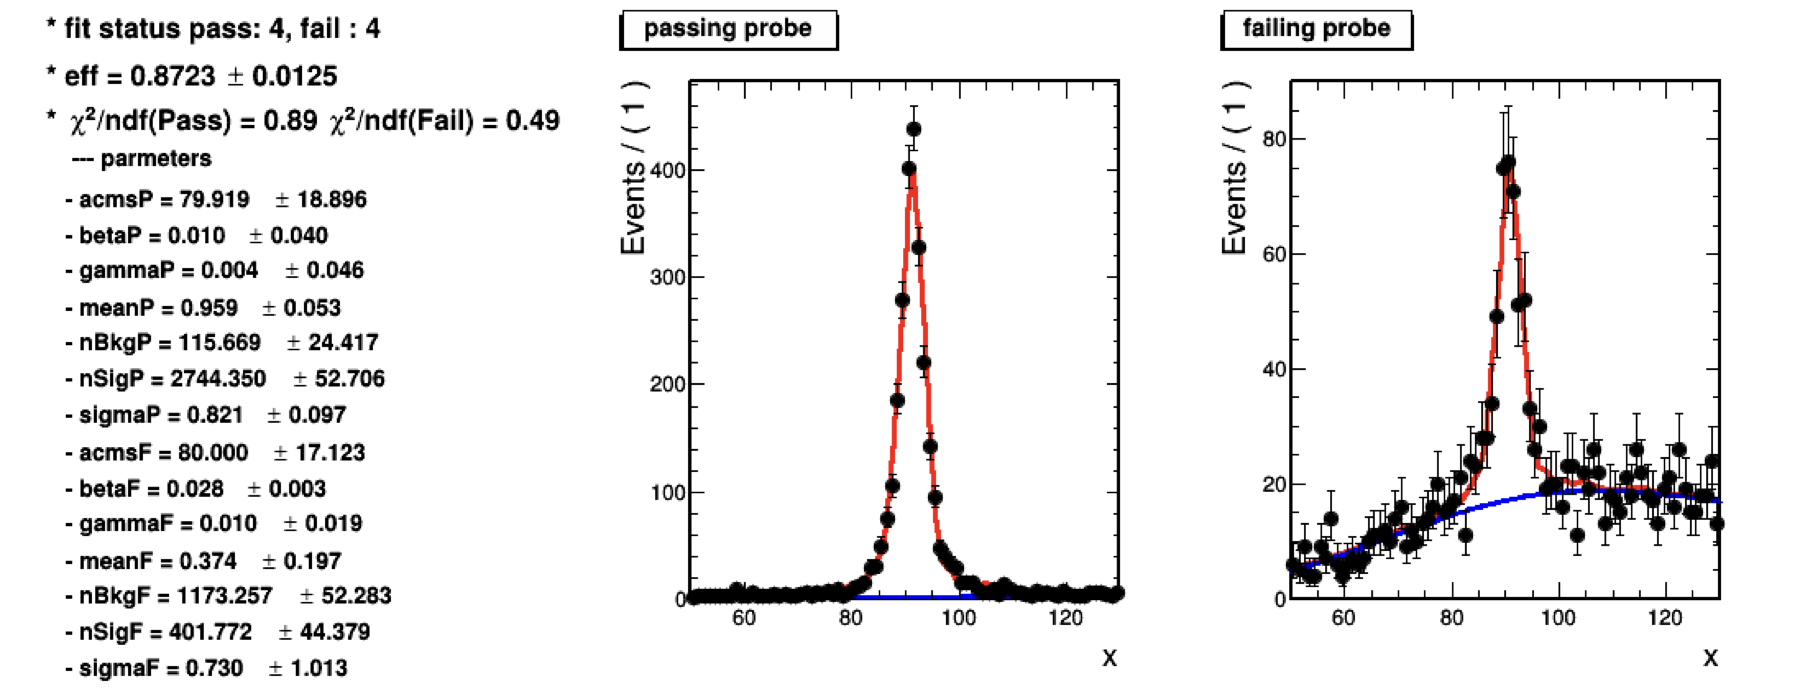
\includegraphics[width=1.0\textwidth]{fig/NominalBkg.png}\\
  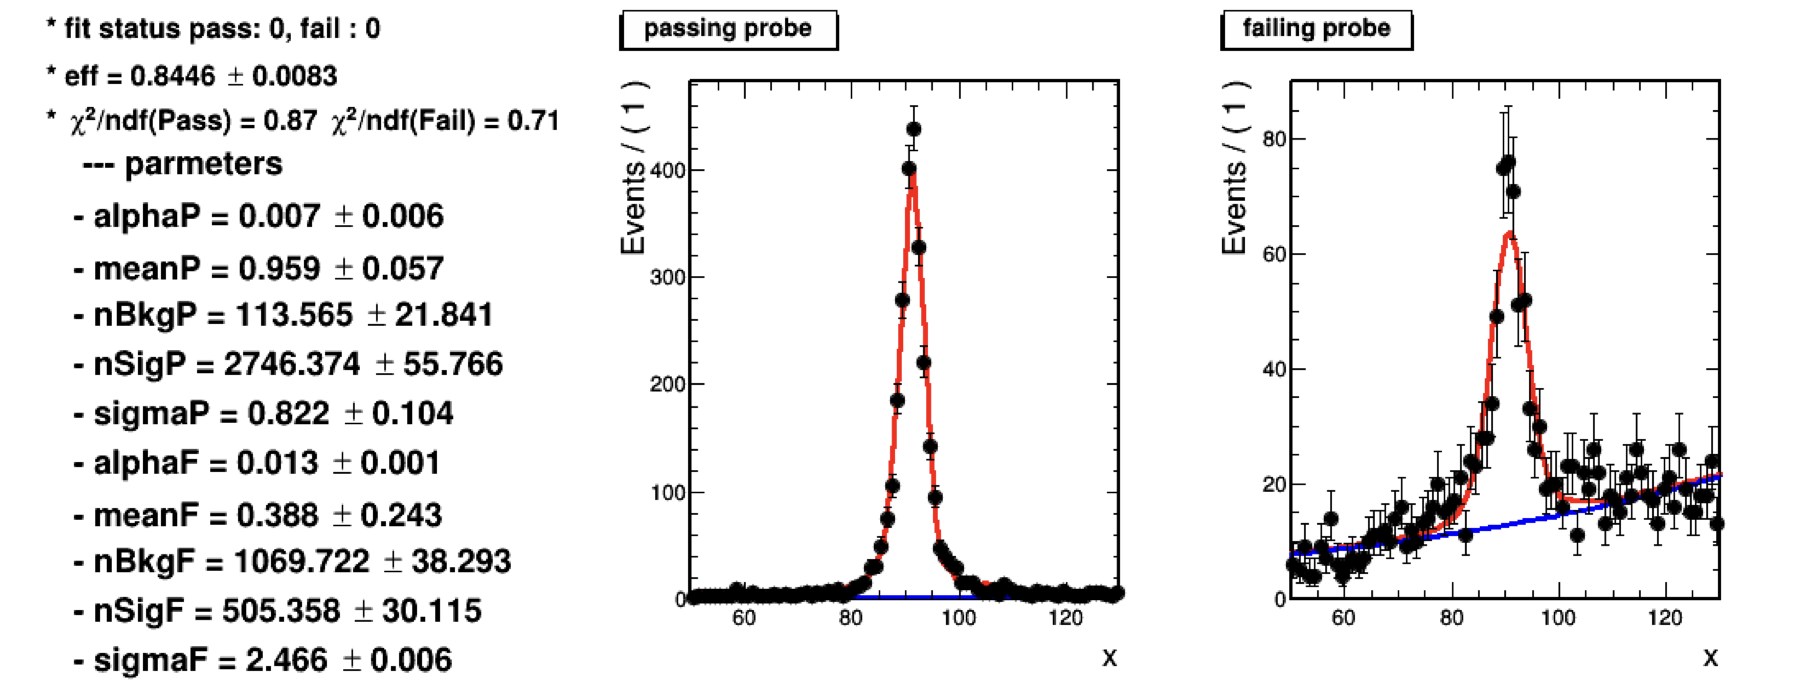
\includegraphics[width=1.0\textwidth]{fig/AltBkg_exponential.png}\\
 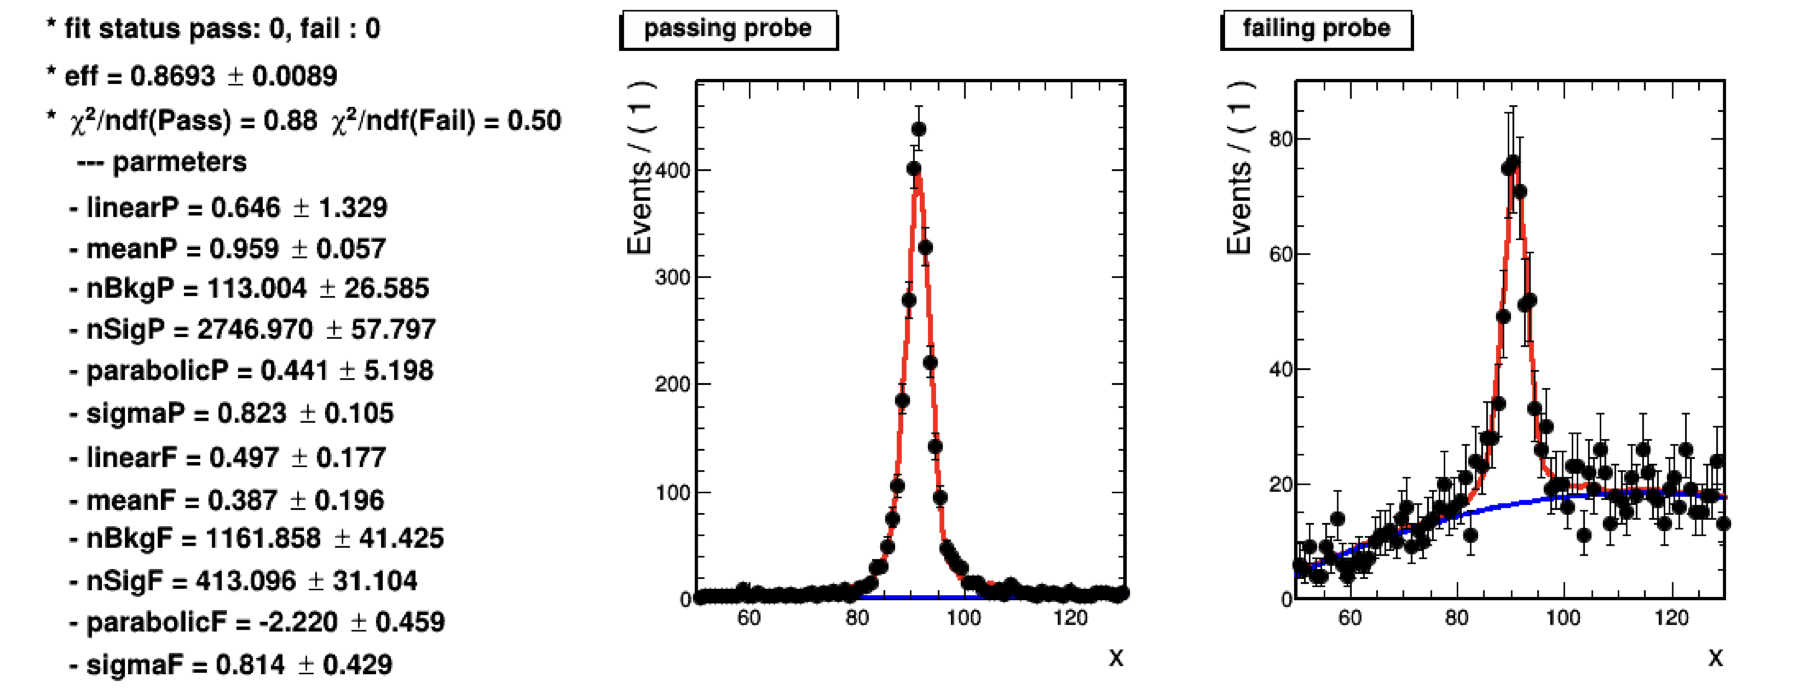
\includegraphics[width=1.0\textwidth]{fig/AltBkg_Polynomial.png}
 
  \label{fig:Sysbkg}
\end{figure}

\begin{figure}[!htbp]
  \centering
 \caption{Extrapolation plots for 2016. (a,b,c) are the extrapolation fitting results. (d,e,f) are consistency checks. The extrapolated scale factors and uncertainties are drawn on top of the tag-and-probe measured results.}
  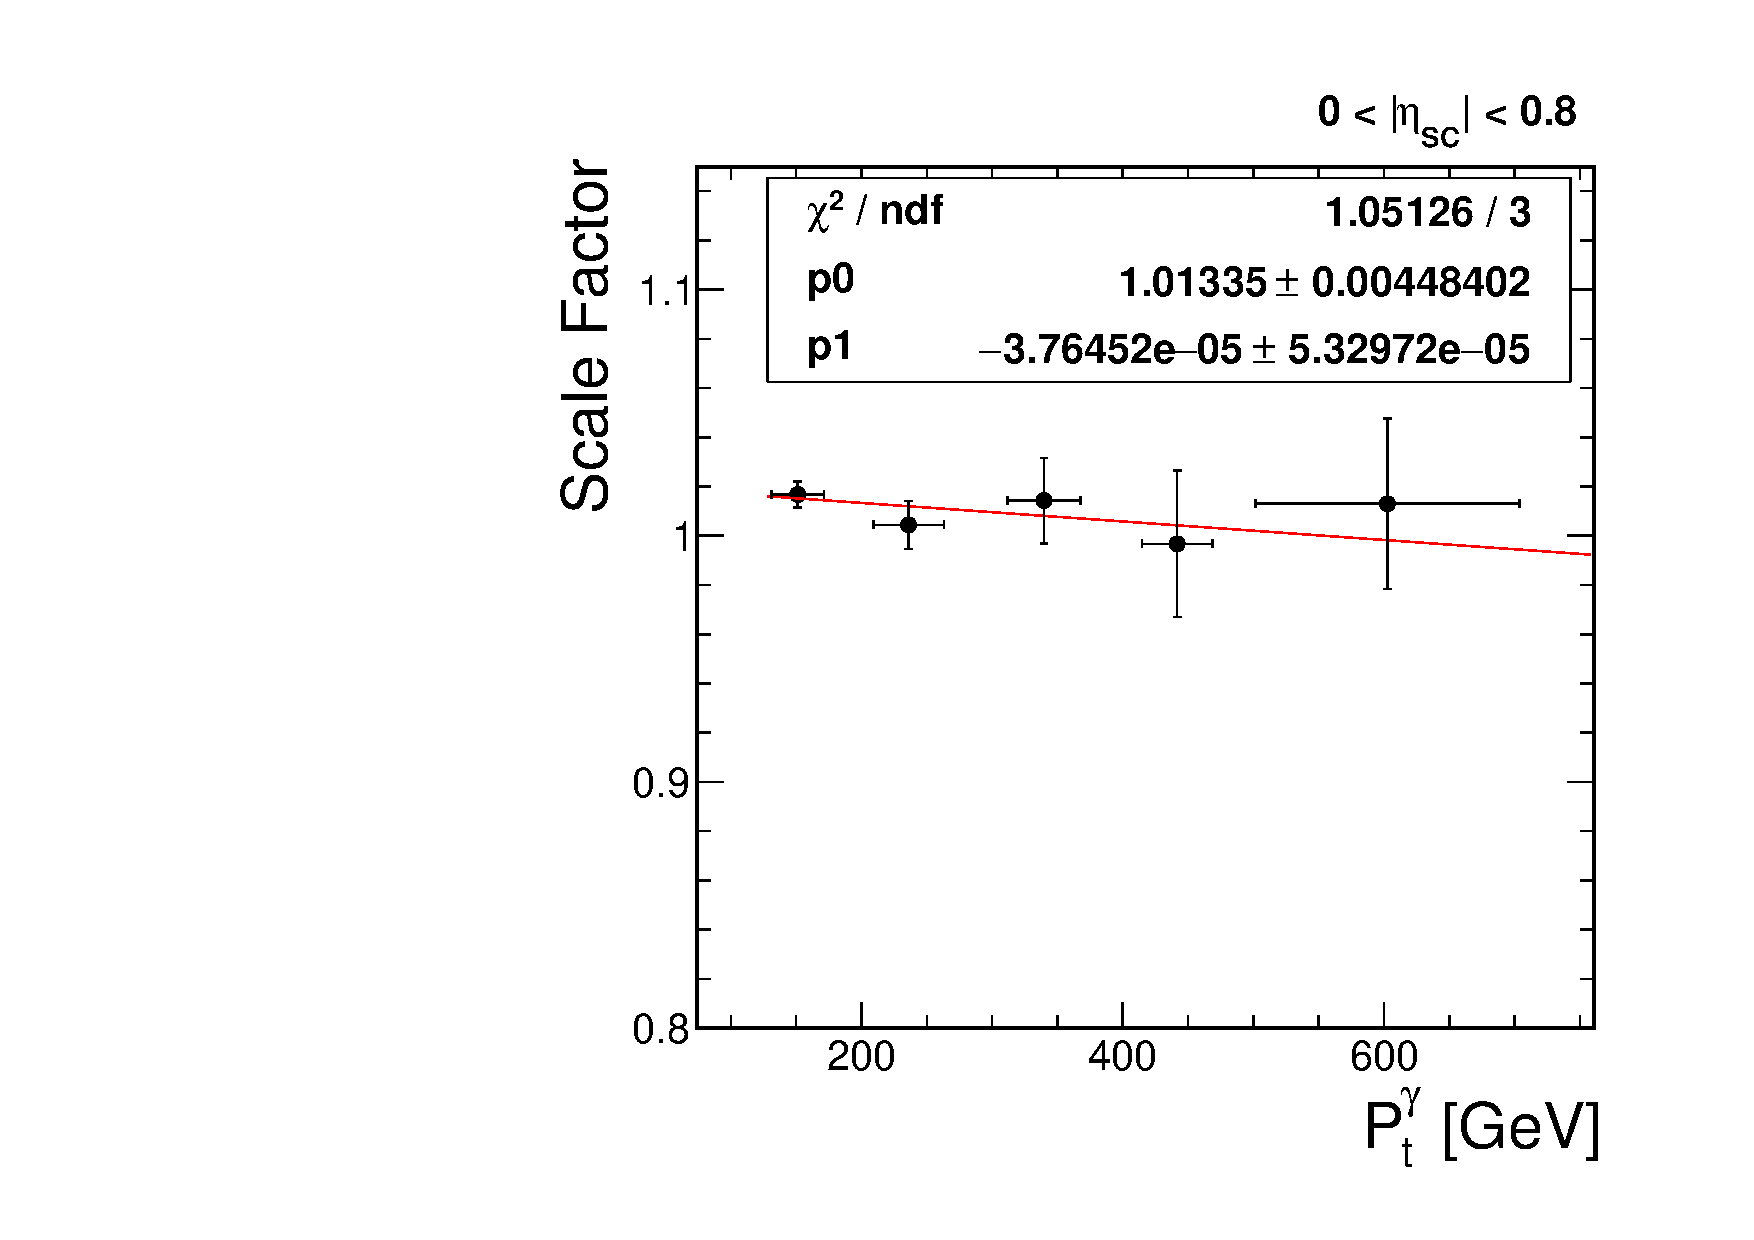
\includegraphics[width=0.3\textwidth]{fig/Extrapolate_2016_0_Fit.pdf}
  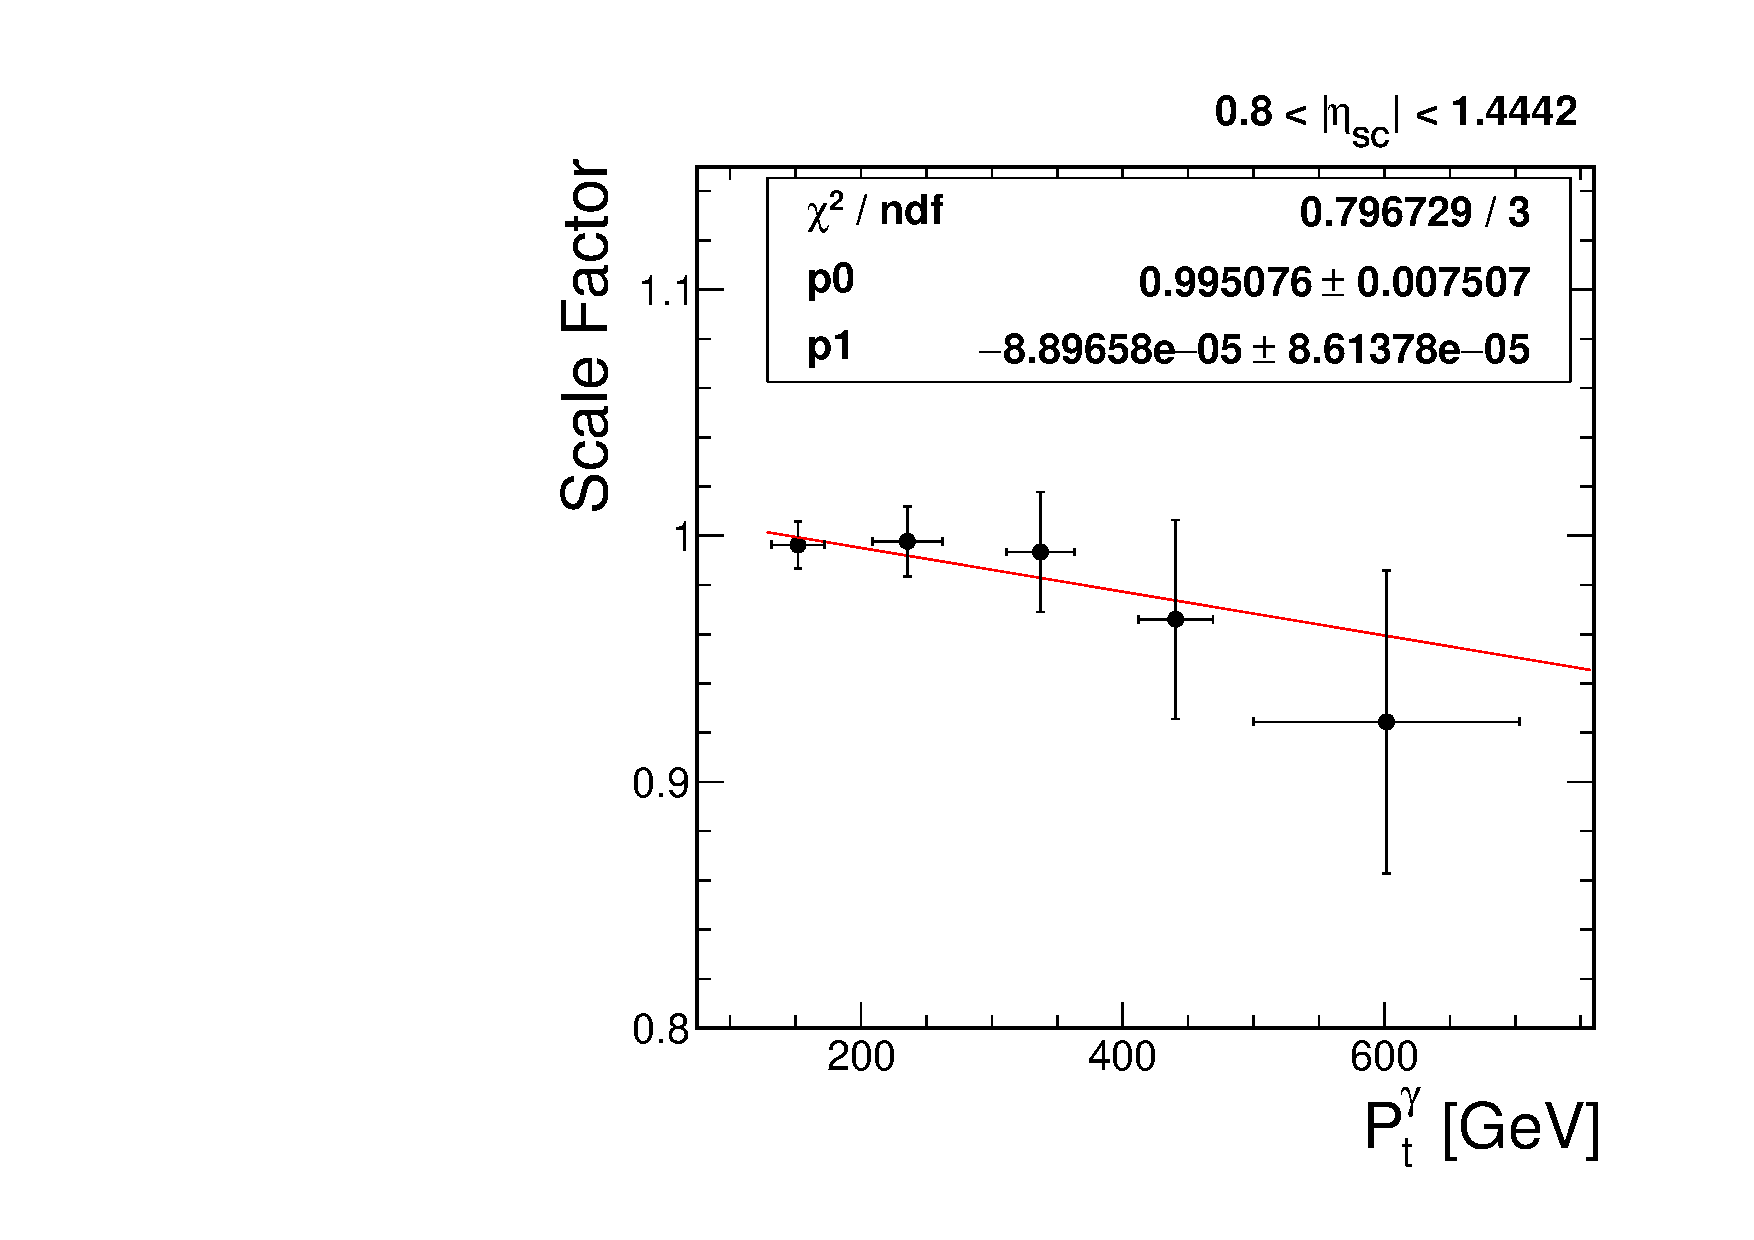
\includegraphics[width=0.3\textwidth]{fig/Extrapolate_2016_1_Fit.pdf}
  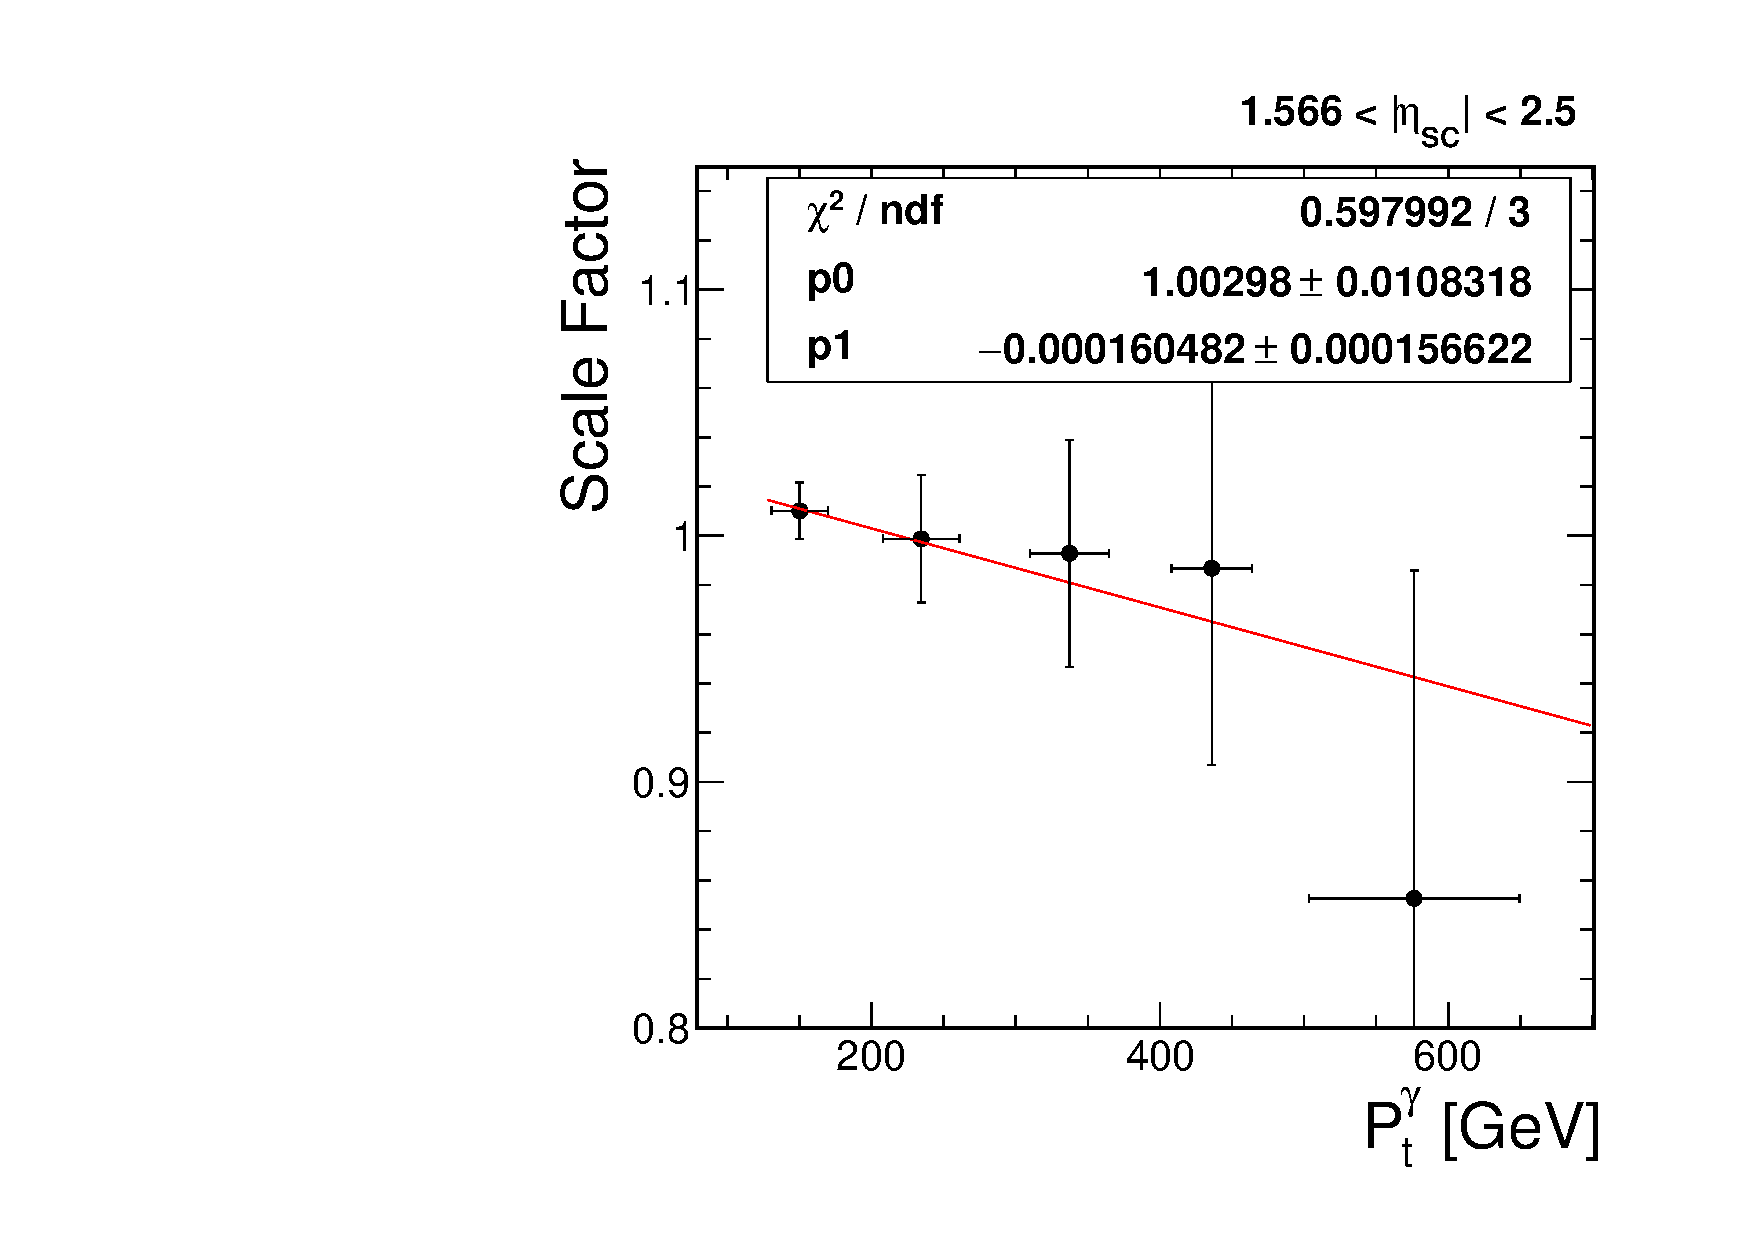
\includegraphics[width=0.3\textwidth]{fig/Extrapolate_2016_2_Fit.pdf}\\
  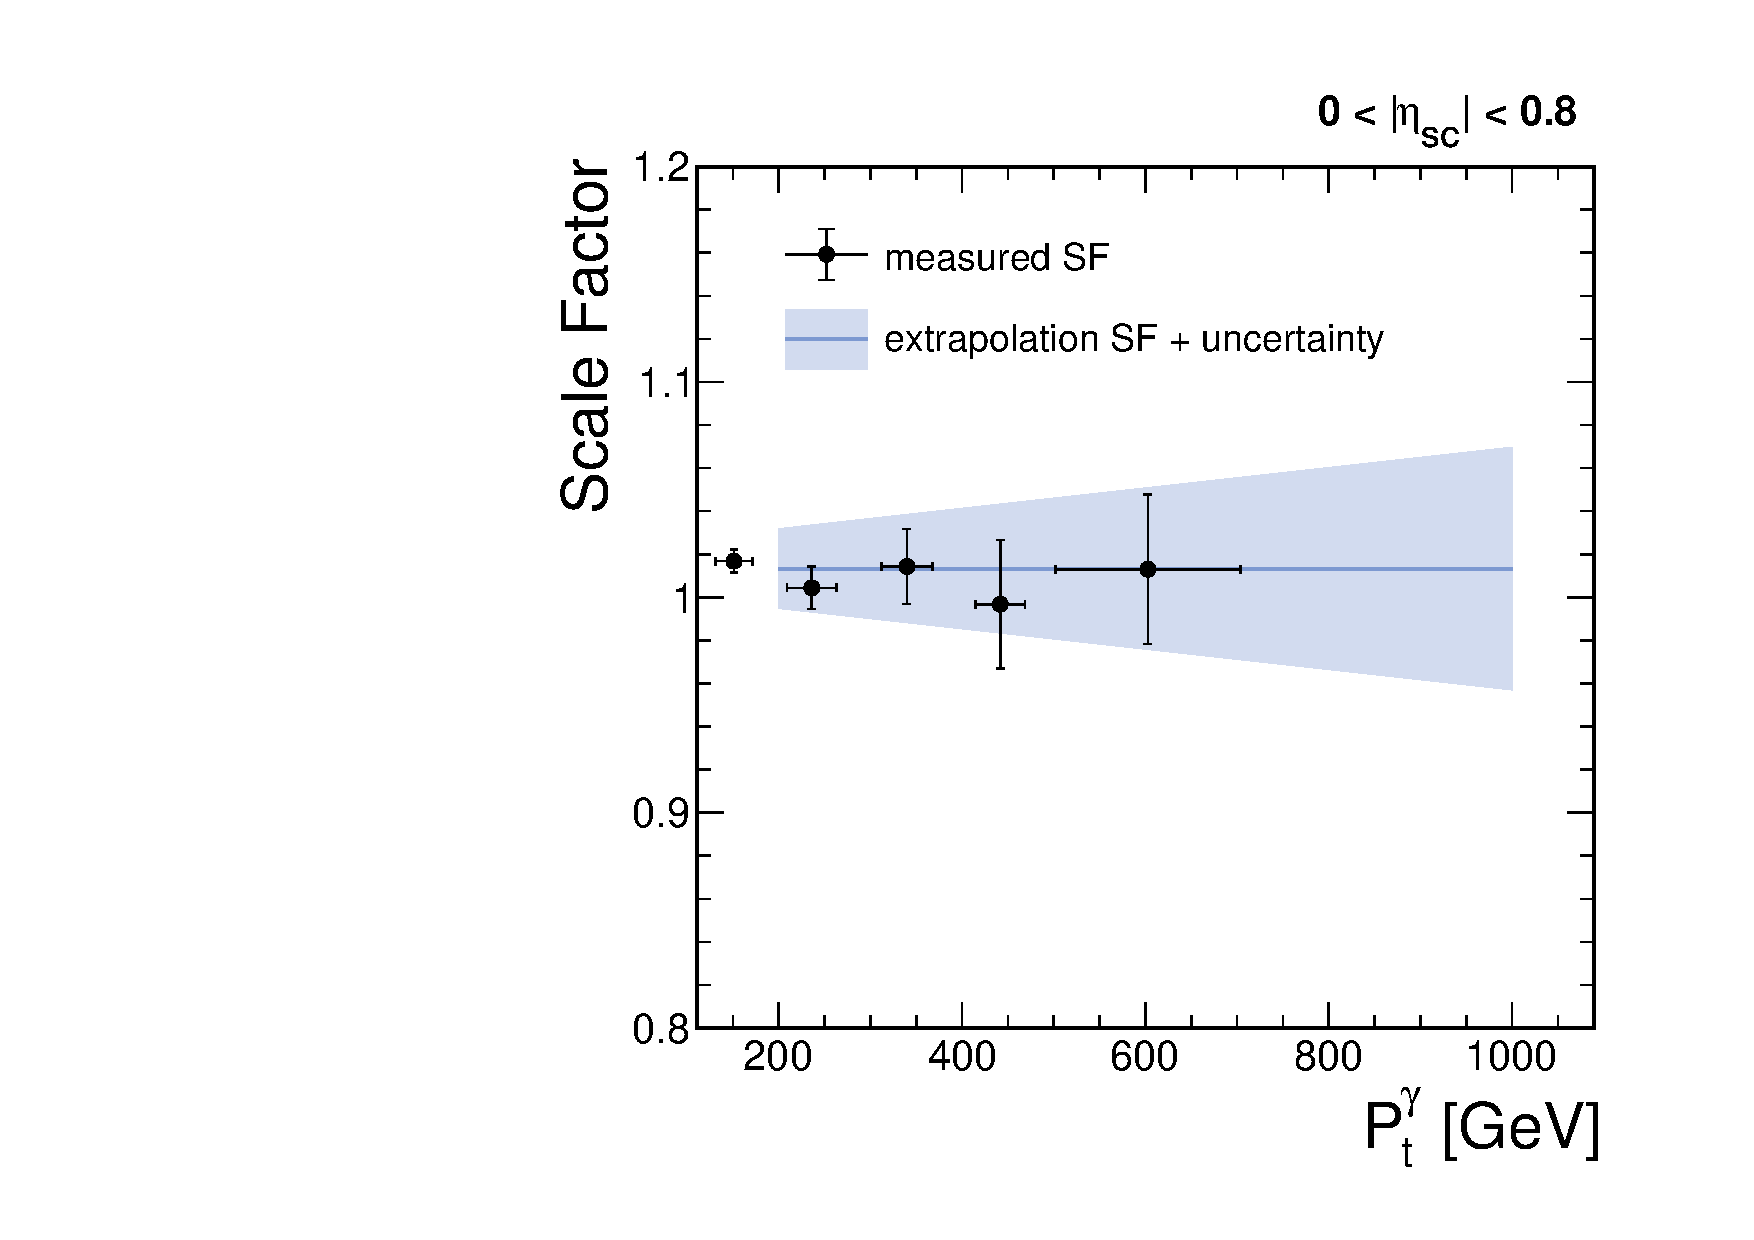
\includegraphics[width=0.3\textwidth]{fig/Extrapolate_2016_0_Check.pdf}
  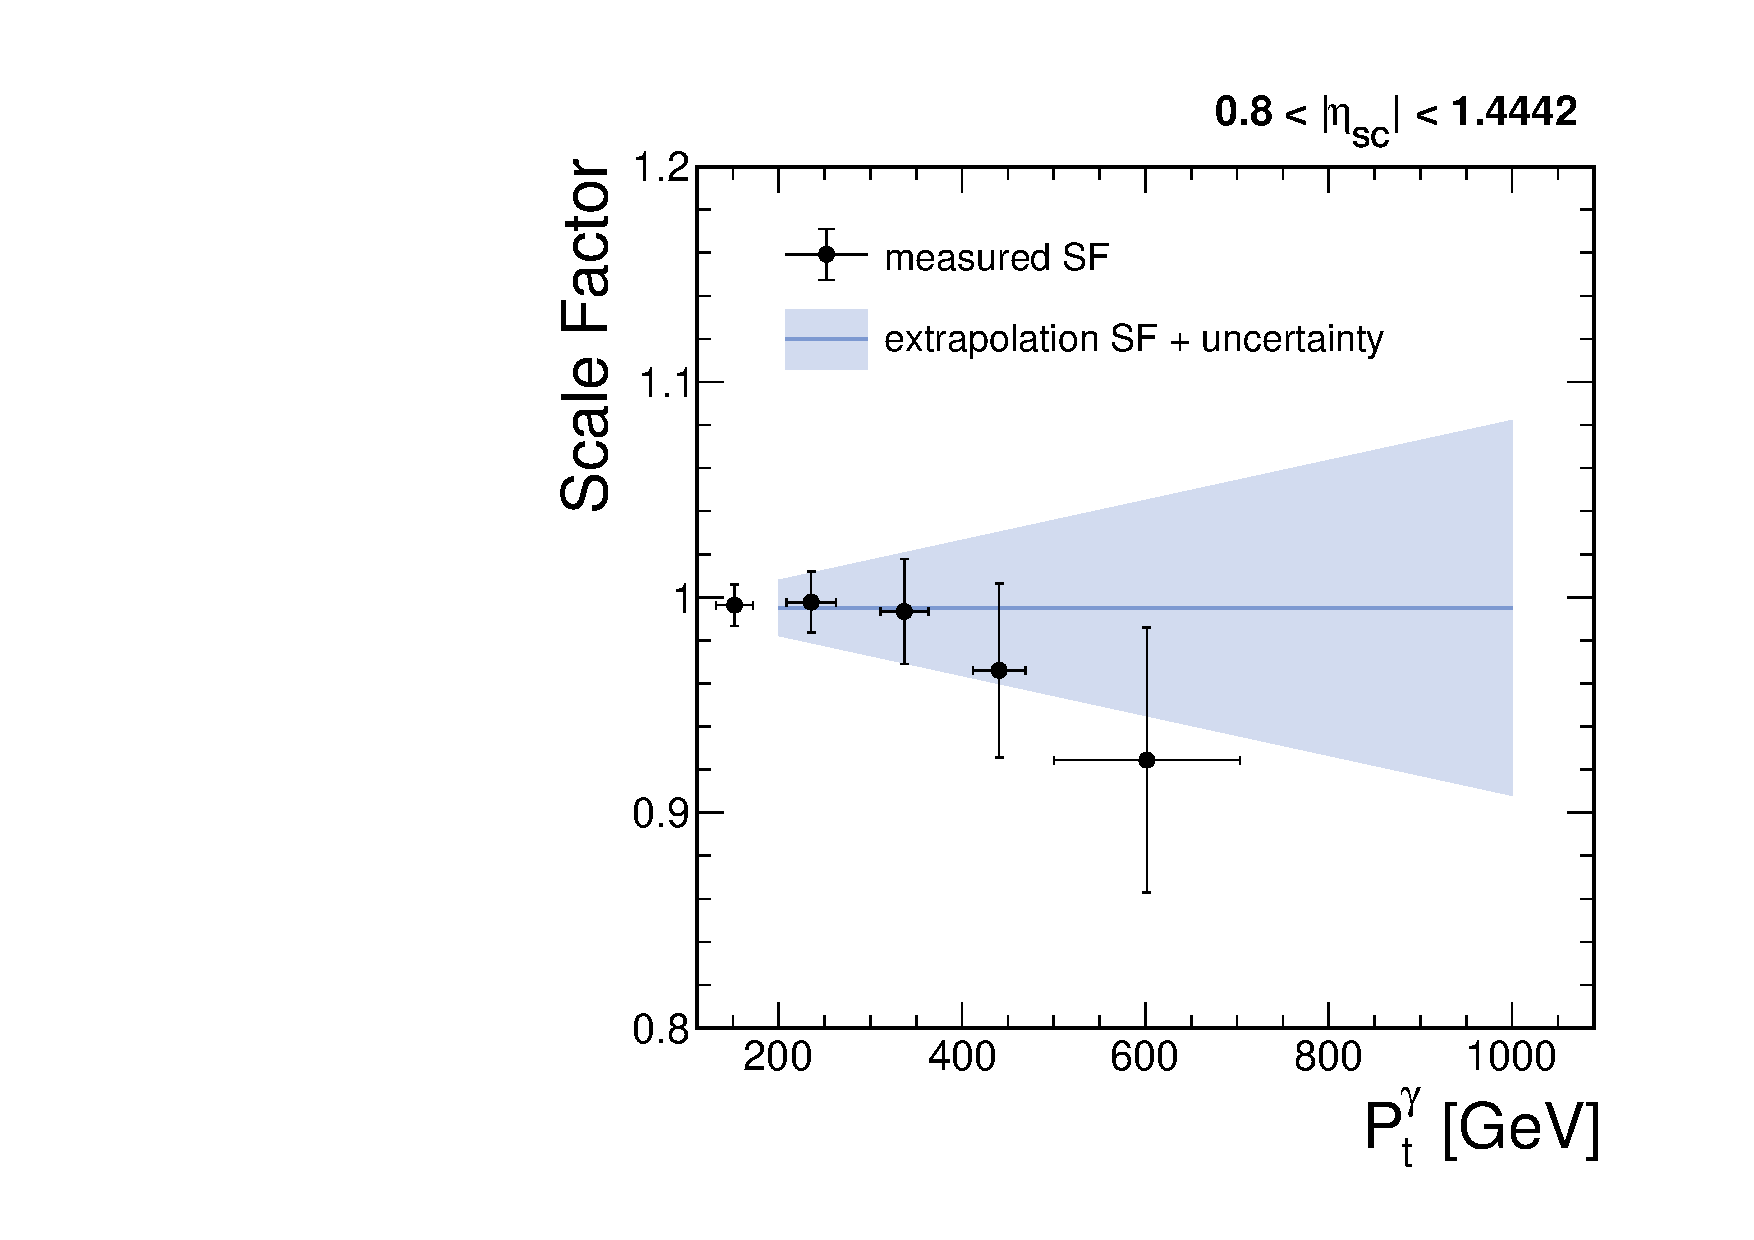
\includegraphics[width=0.3\textwidth]{fig/Extrapolate_2016_1_Check.pdf}
  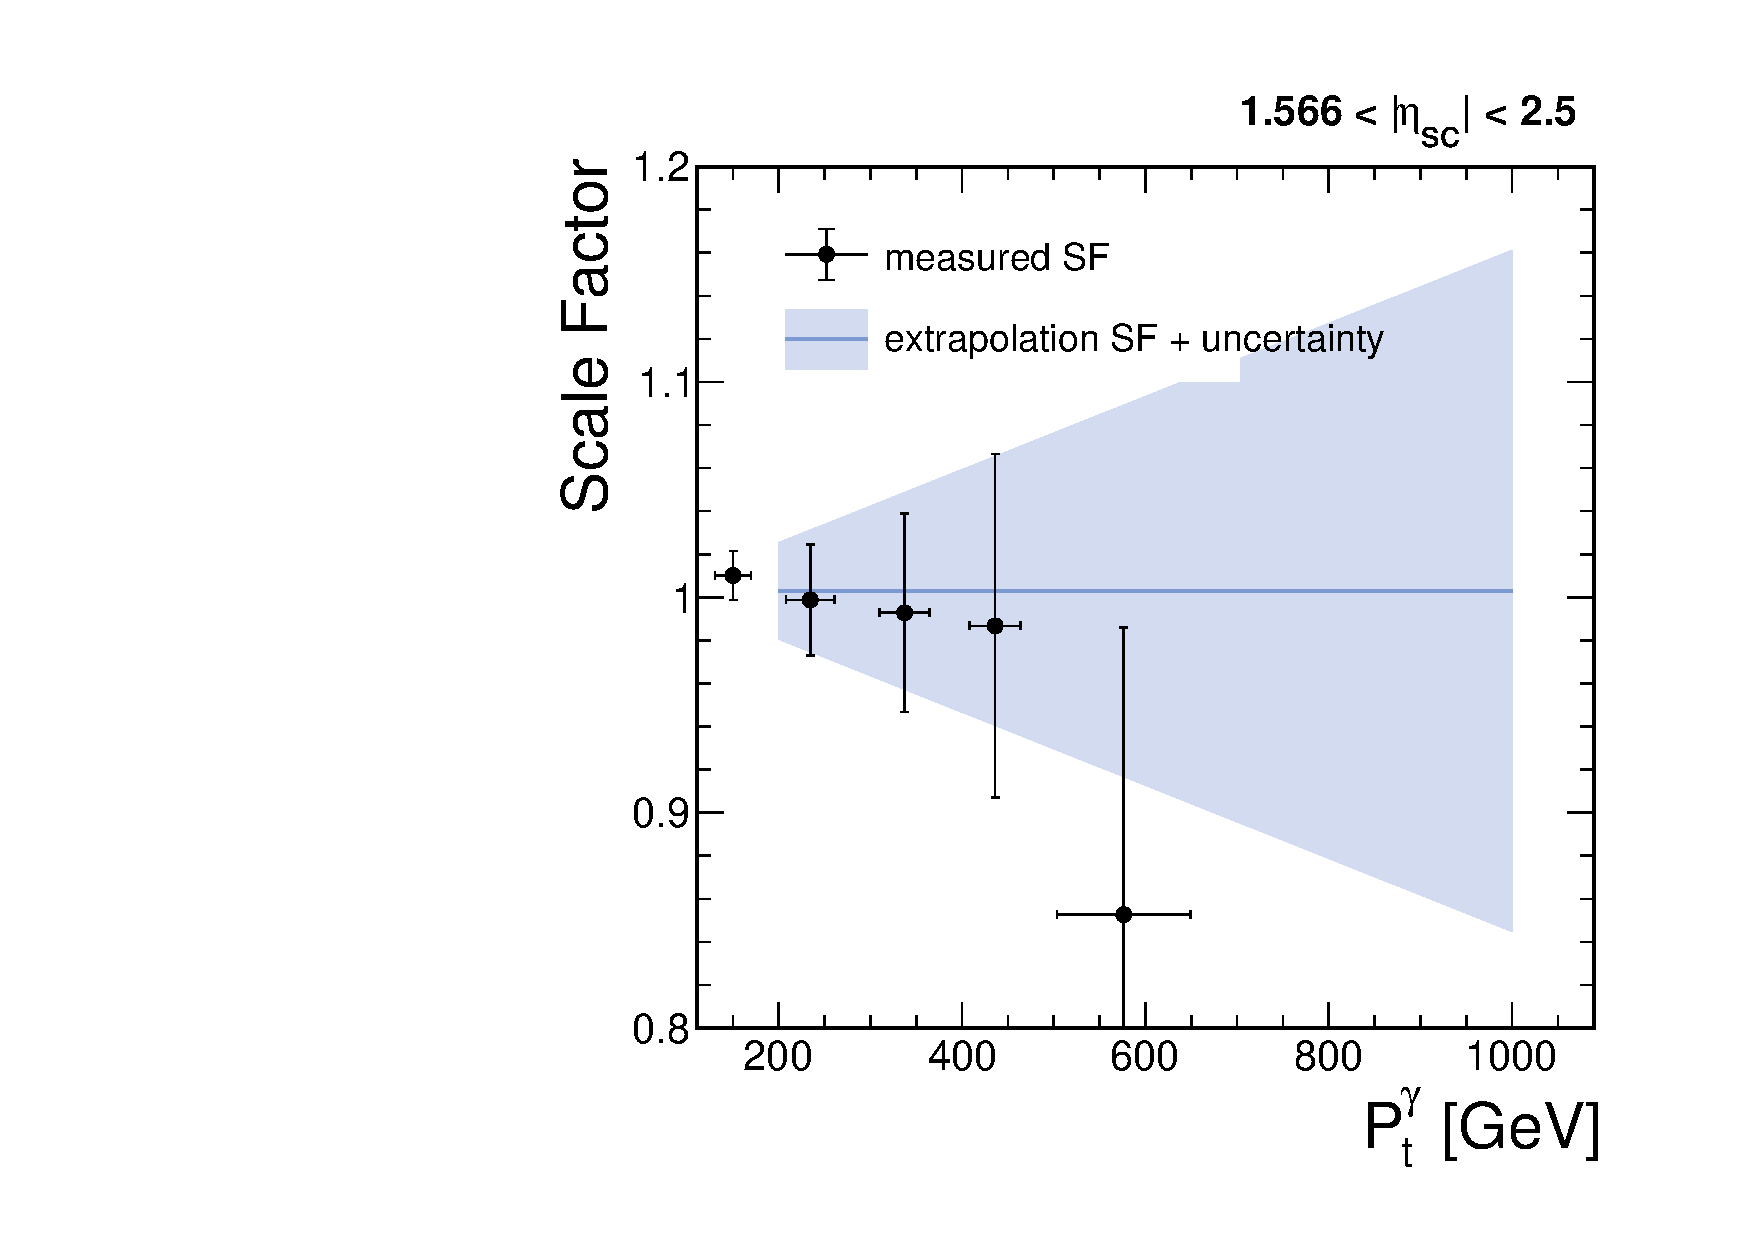
\includegraphics[width=0.3\textwidth]{fig/Extrapolate_2016_2_Check.pdf}\\
  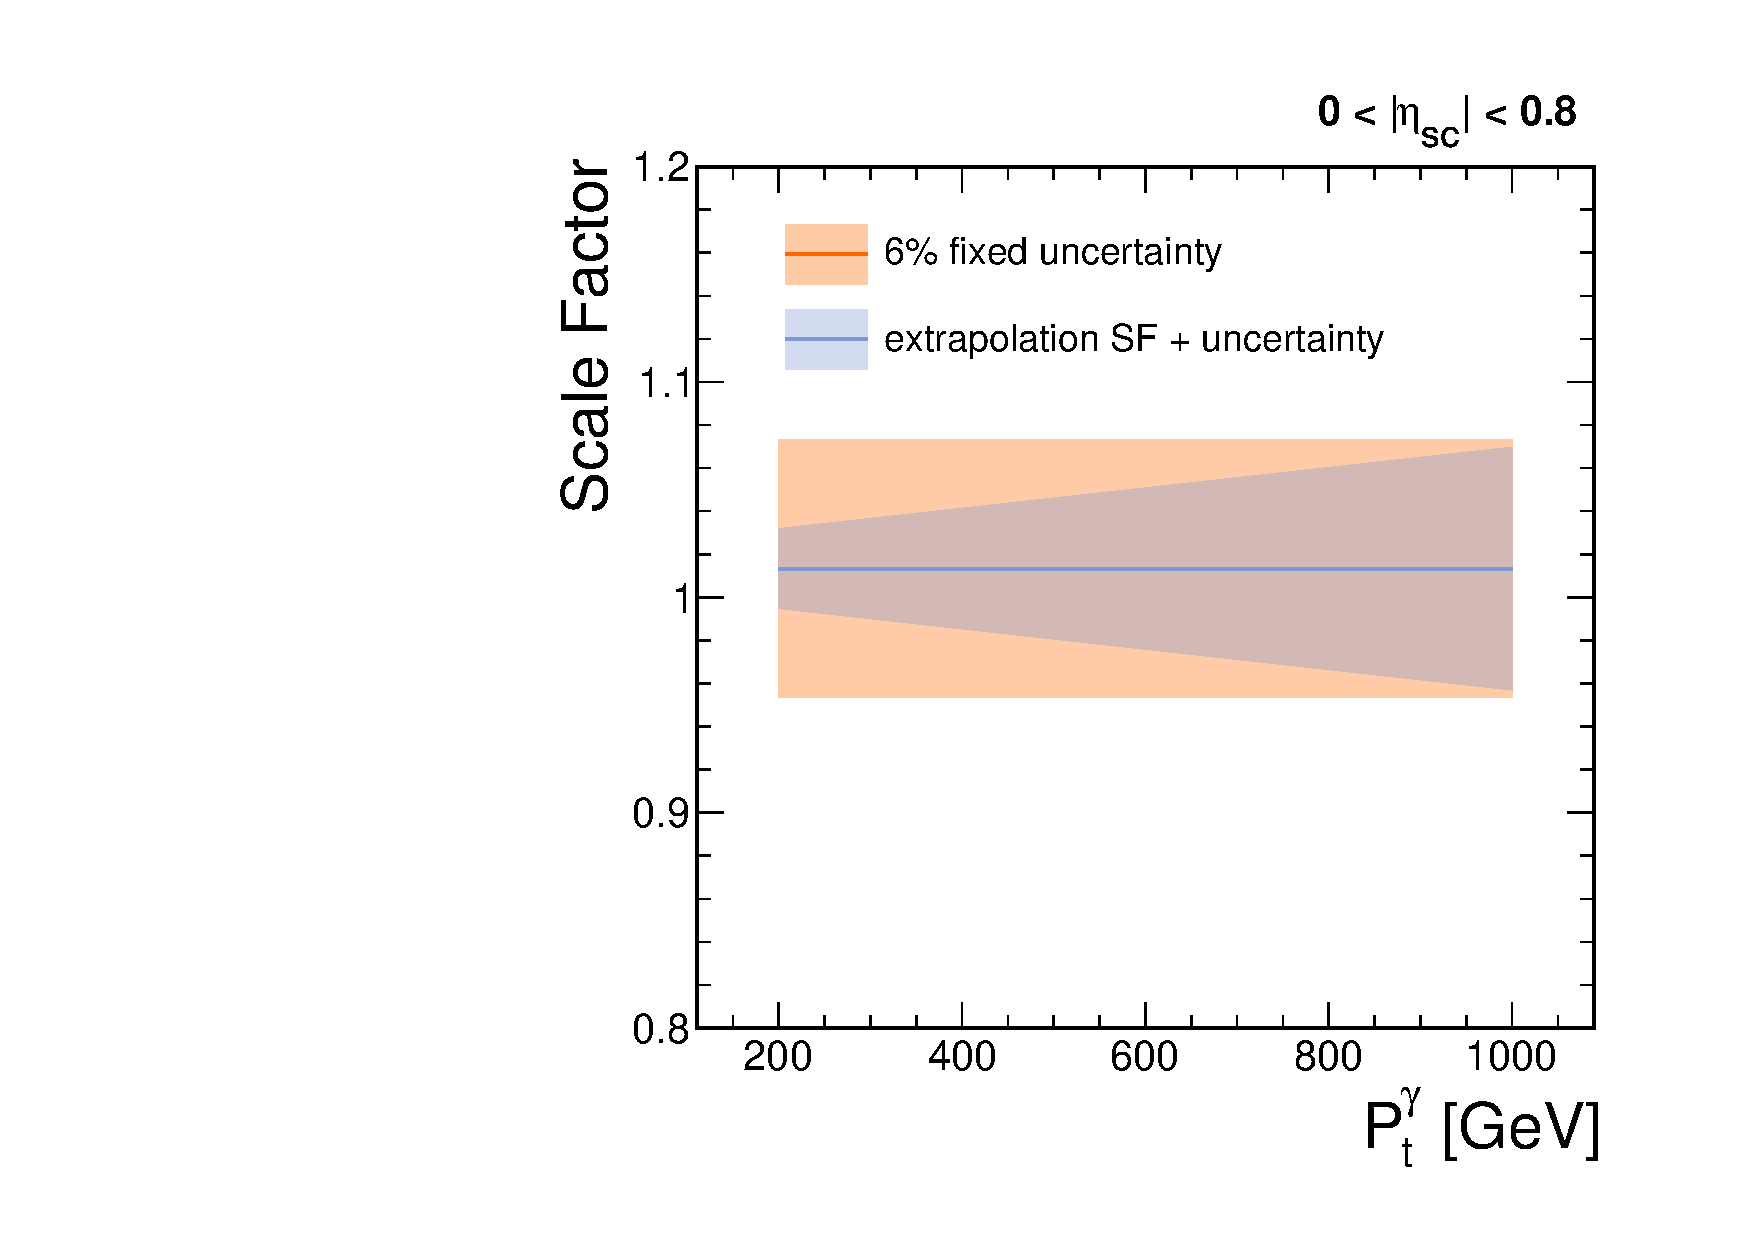
\includegraphics[width=0.3\textwidth]{fig/Extrapolate_2016_0_Compare.pdf}
  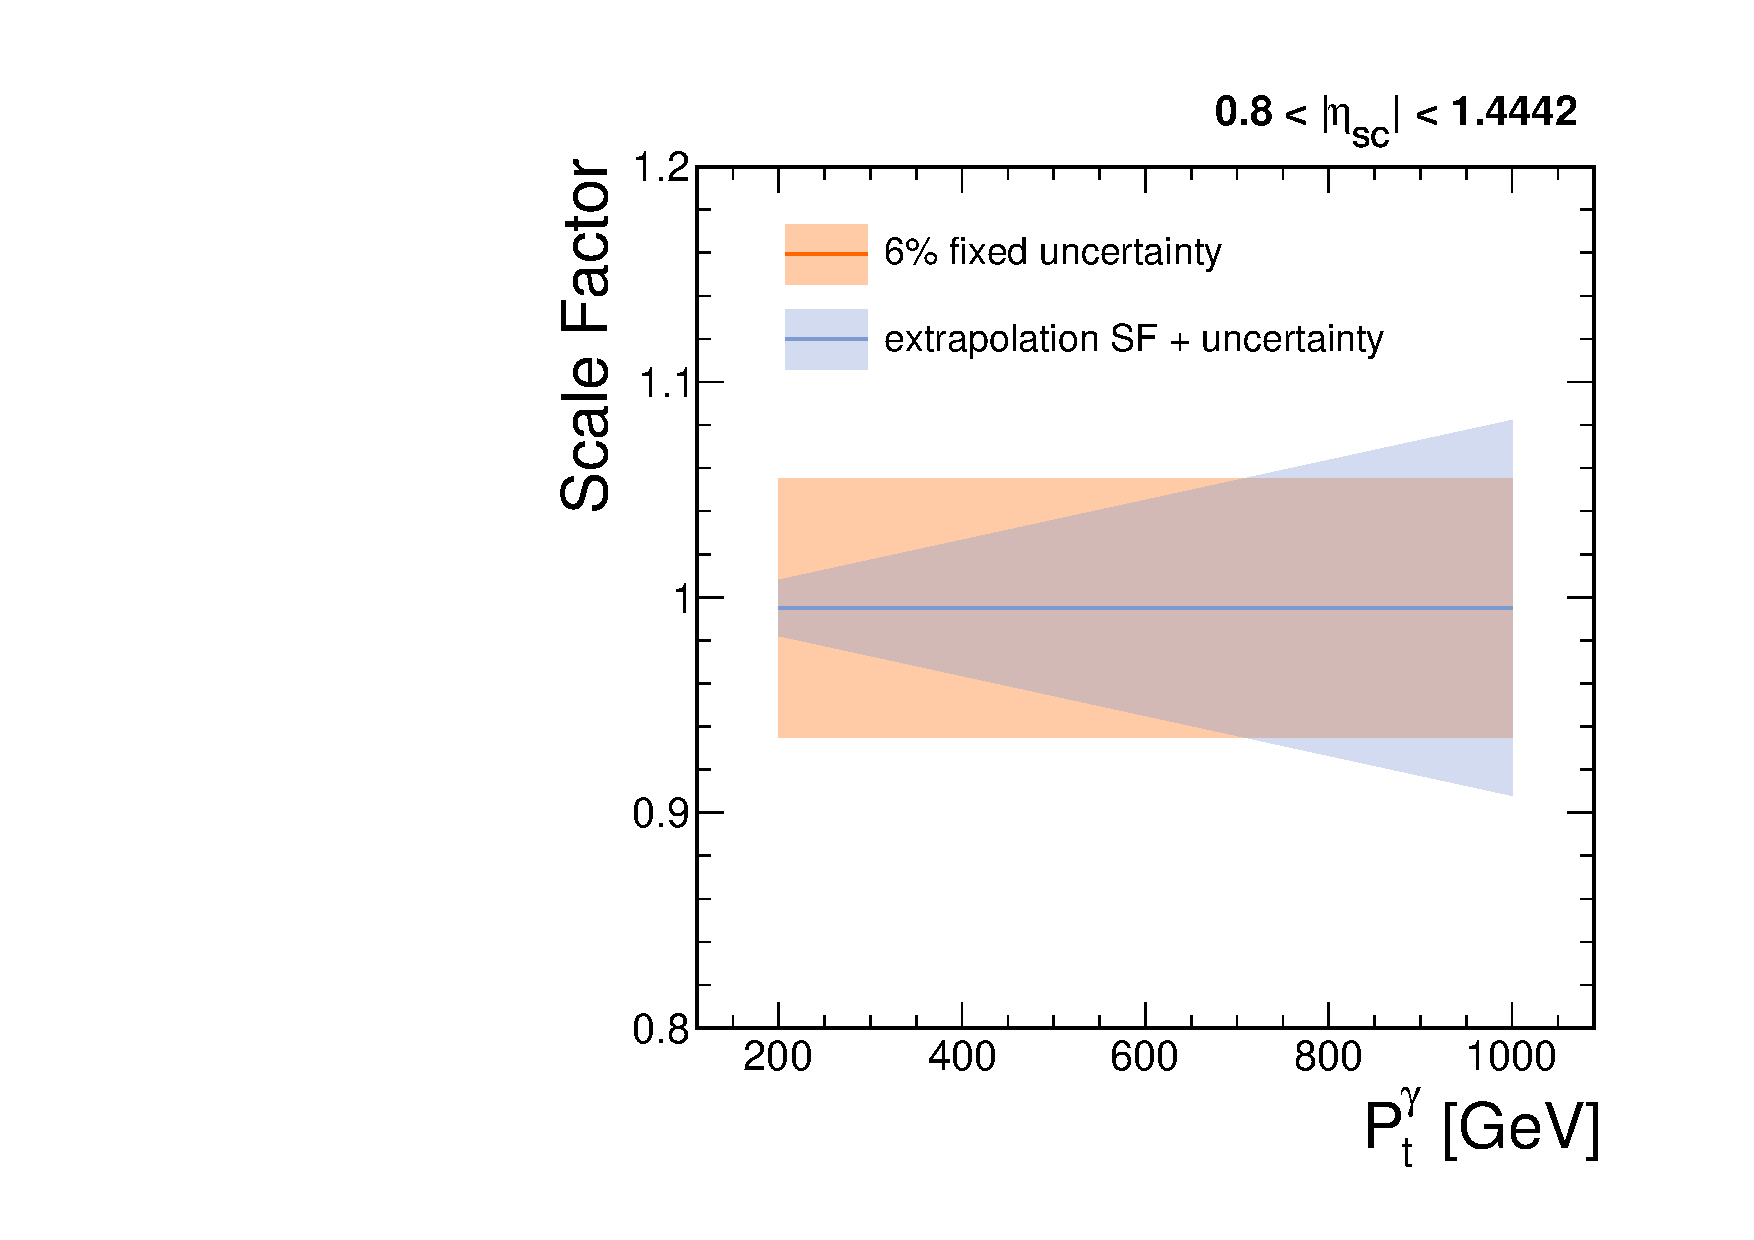
\includegraphics[width=0.3\textwidth]{fig/Extrapolate_2016_1_Compare.pdf}
  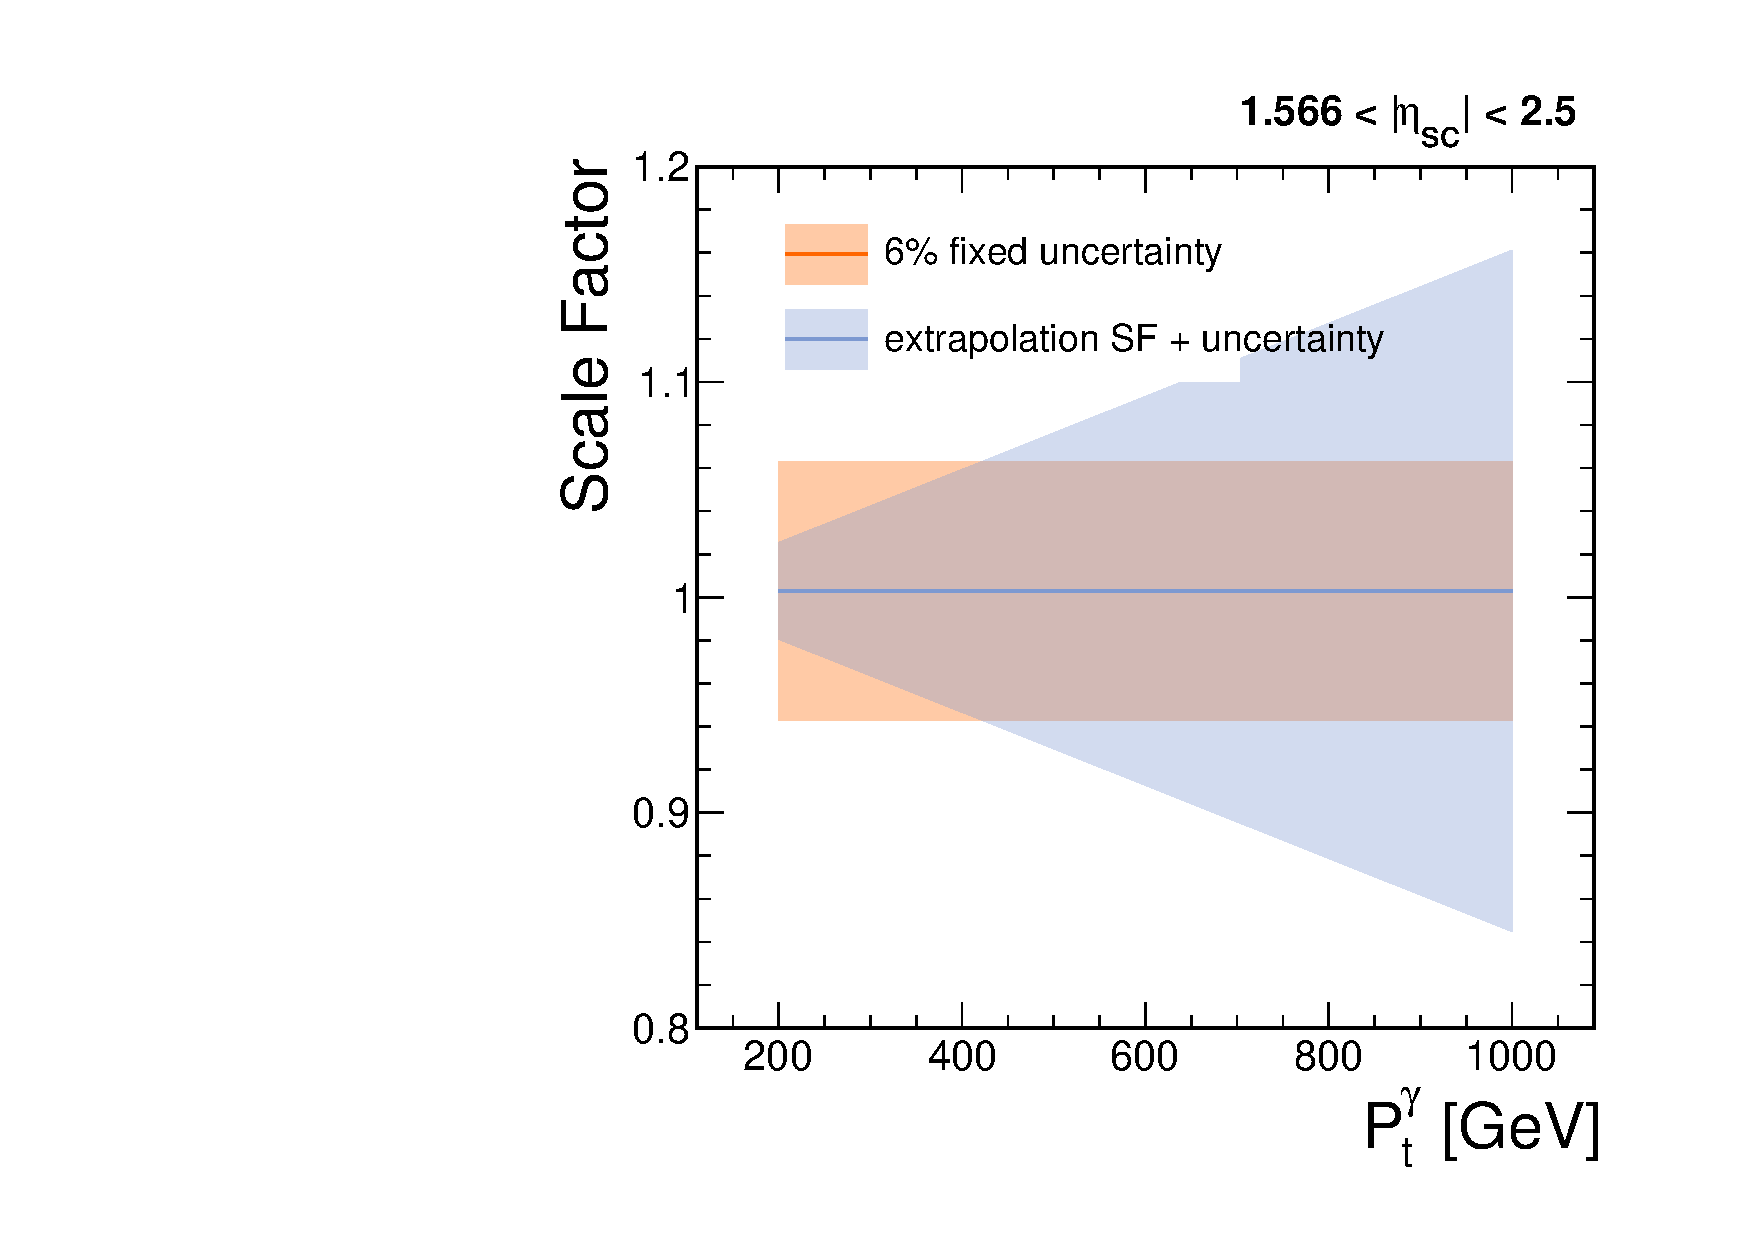
\includegraphics[width=0.3\textwidth]{fig/Extrapolate_2016_2_Compare.pdf}
  \label{fig:Extrapolation}
\end{figure}

\begin{figure}[!htbp]
  \centering
   \caption{Extrapolation plots for 2017. (a,b,c) are the extrapolation fitting results. (d,e,f) are consistency checks. The extrapolated scale factors and uncertainties are drawn on top of the tag-and-probe measured results.}
  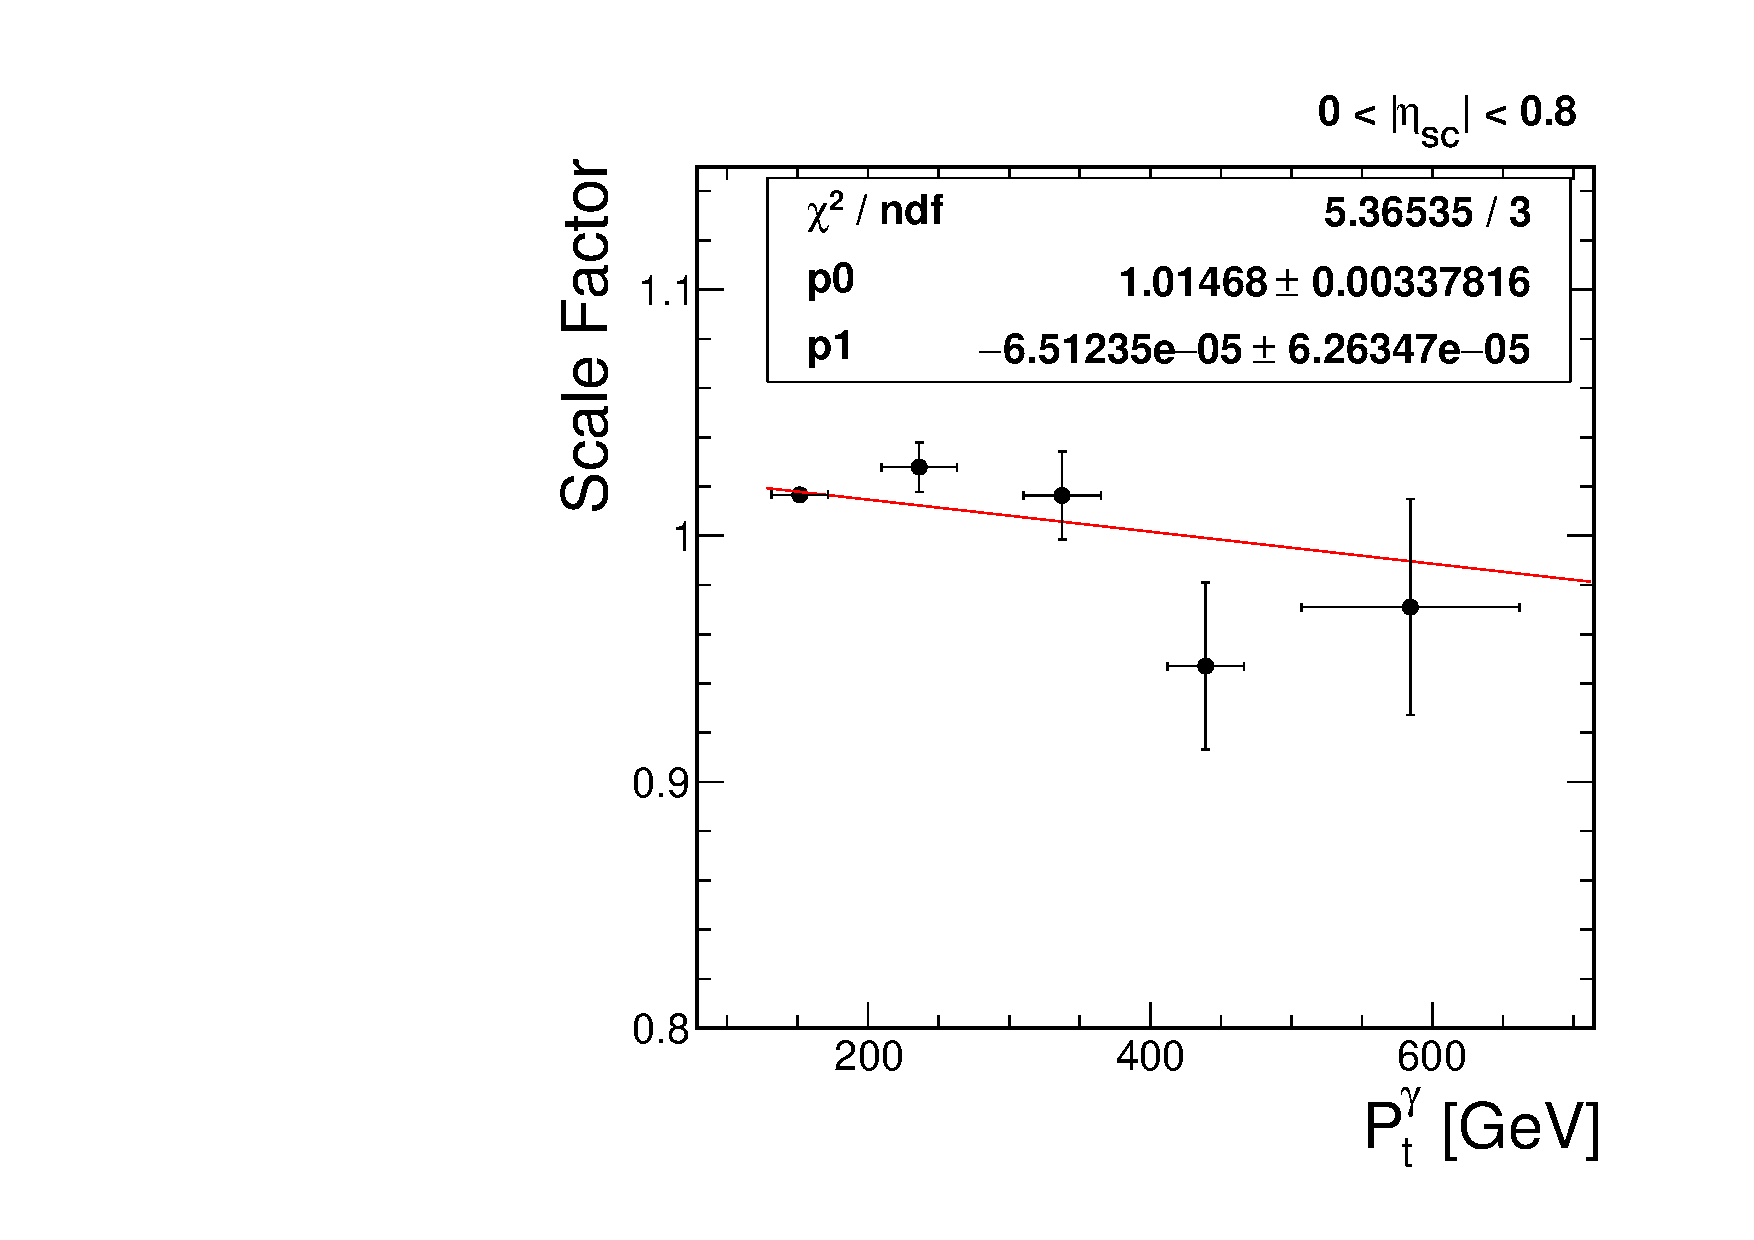
\includegraphics[width=0.3\textwidth]{fig/Extrapolate_2017_0_Fit.pdf}
  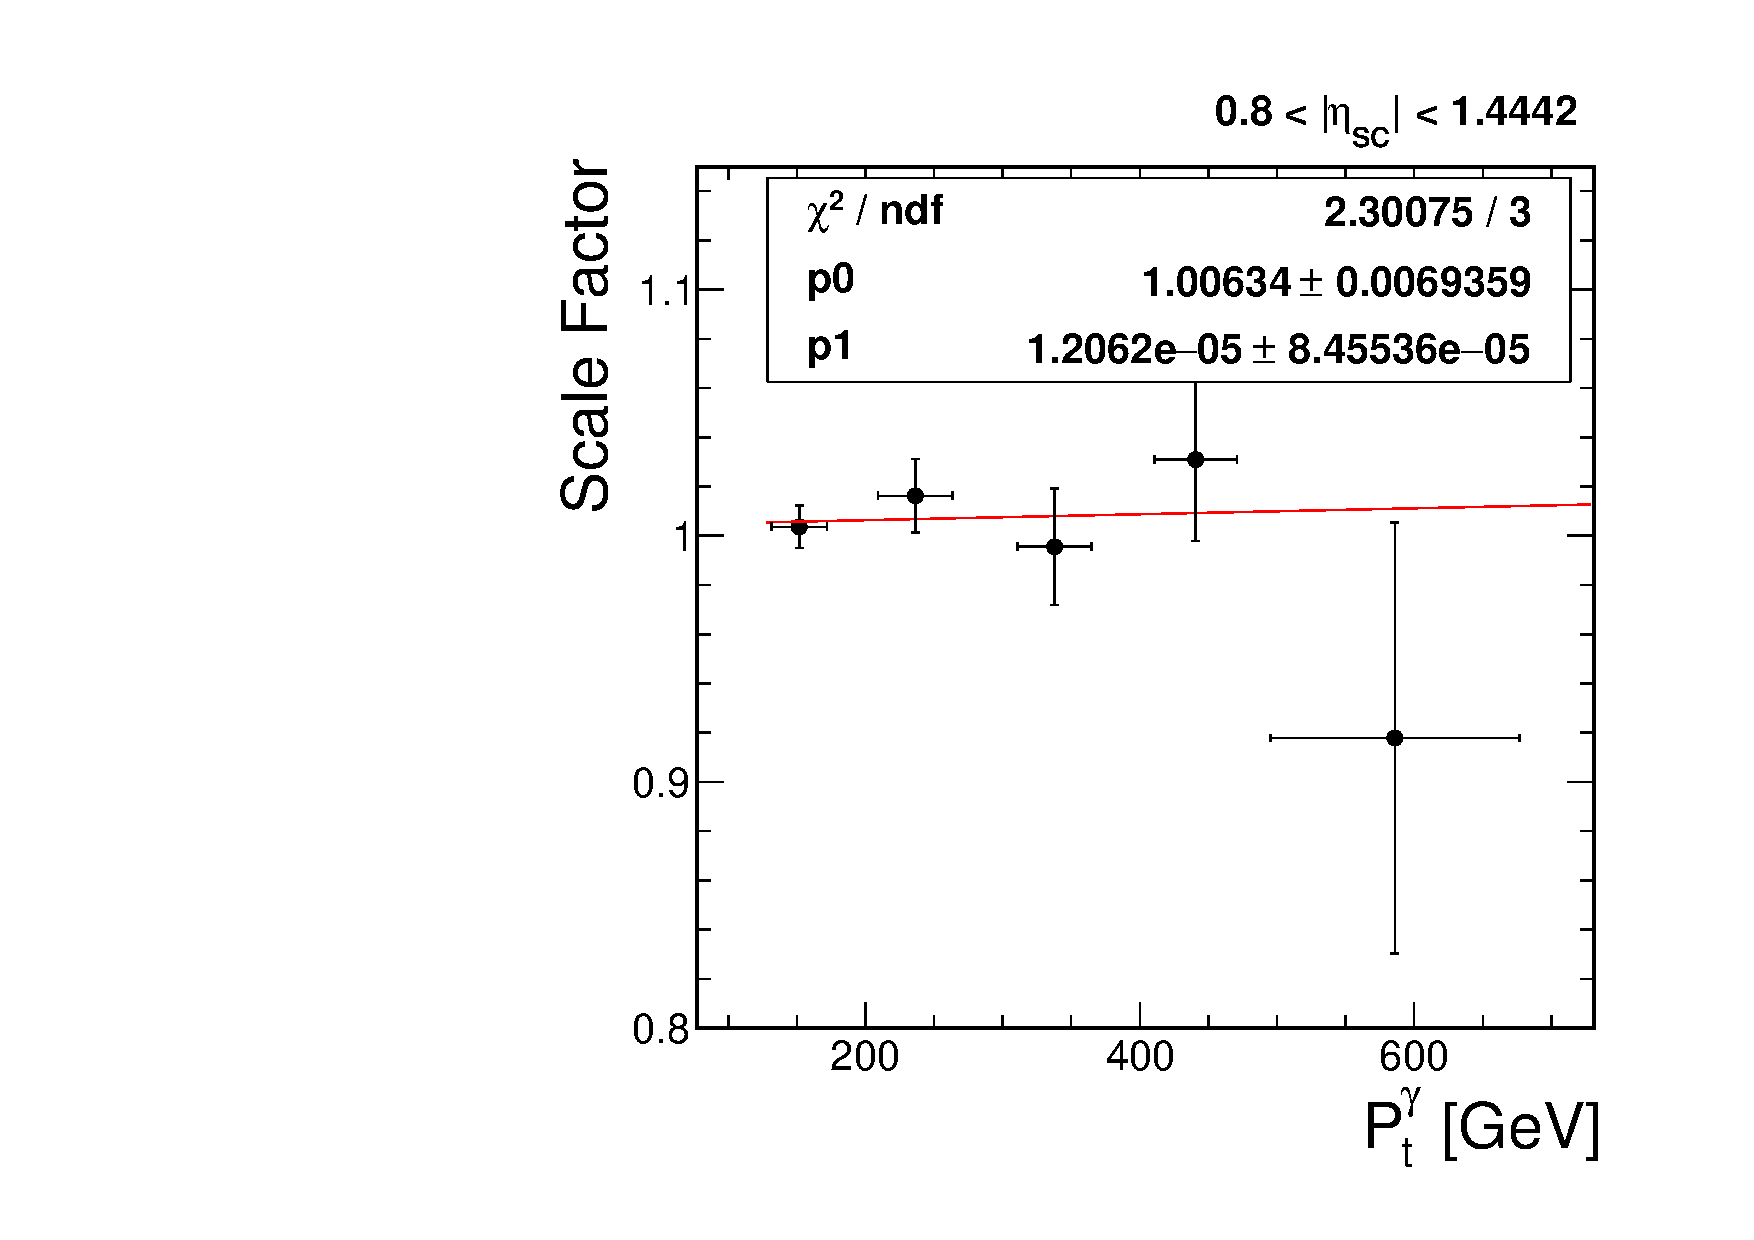
\includegraphics[width=0.3\textwidth]{fig/Extrapolate_2017_1_Fit.pdf}
  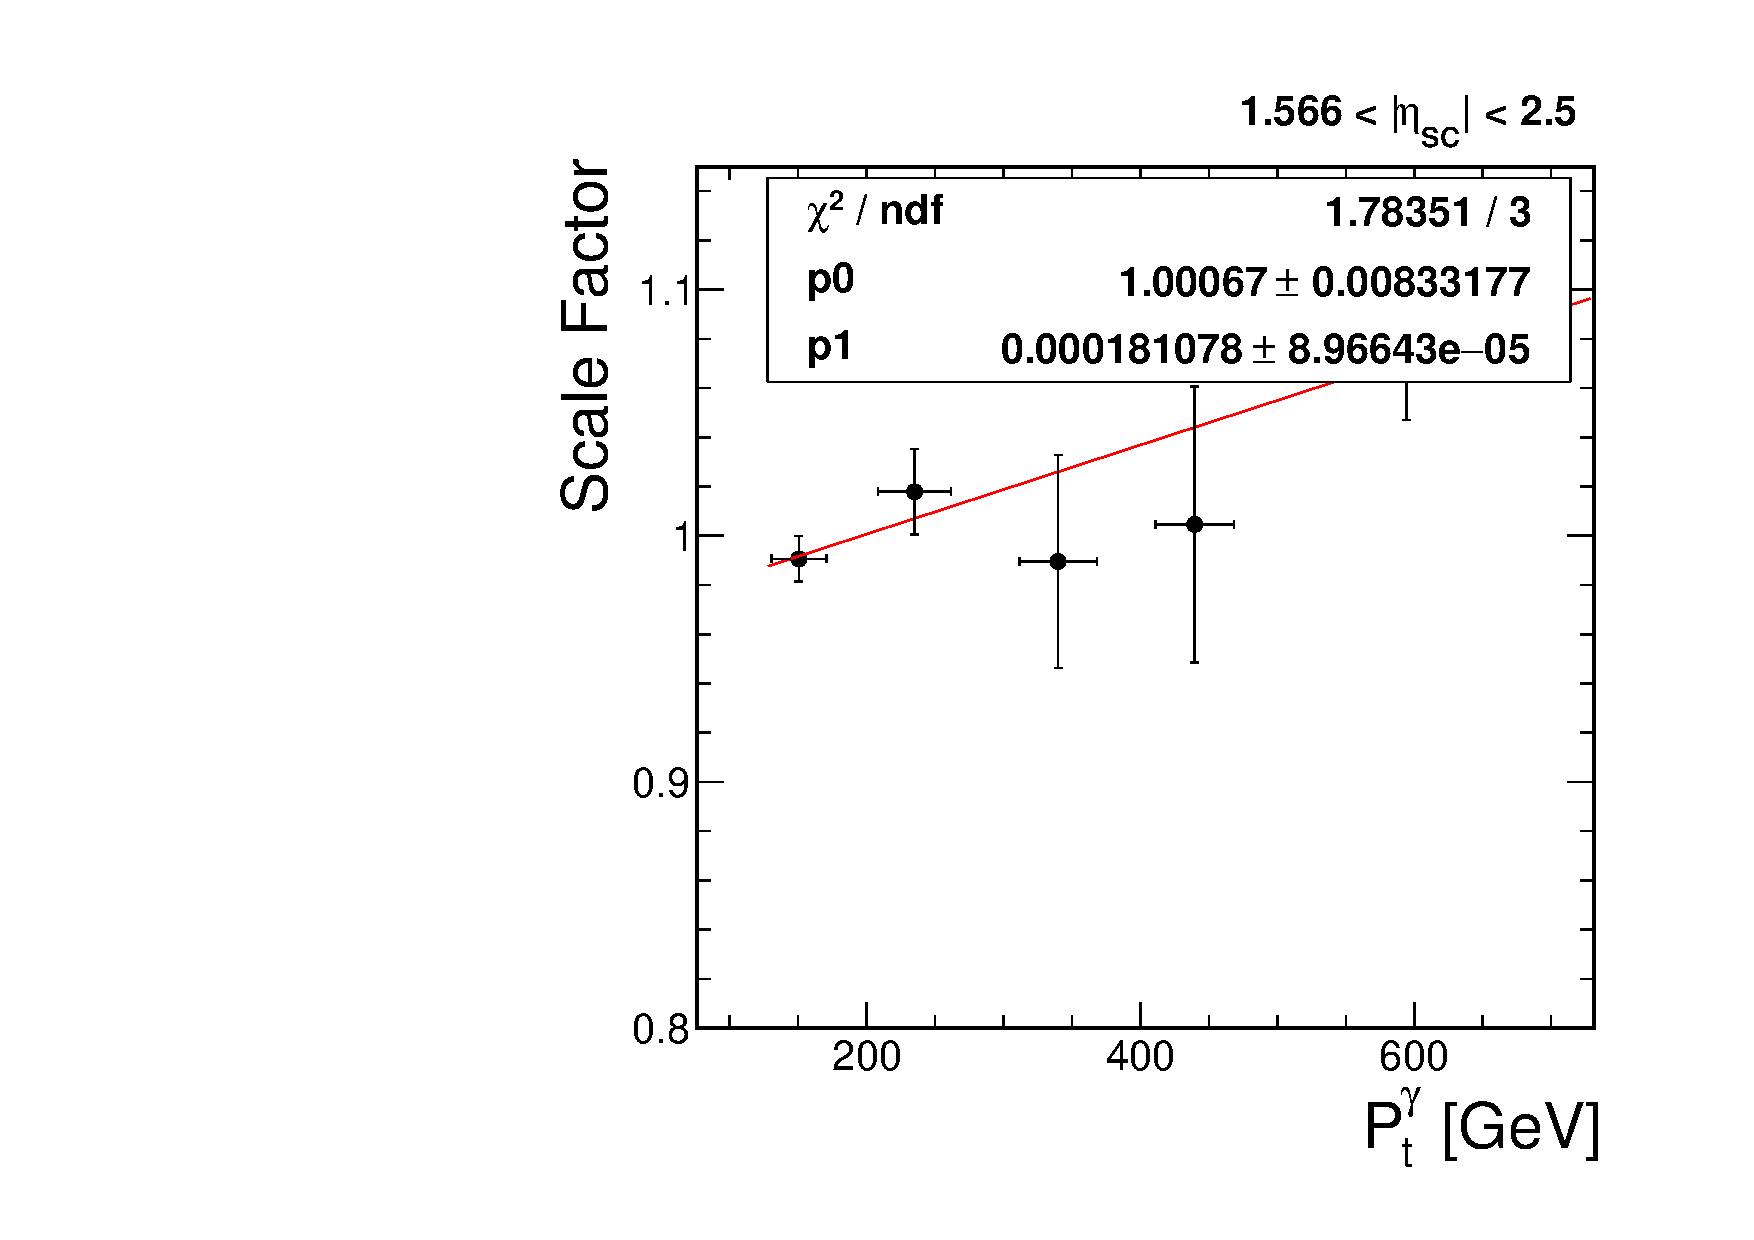
\includegraphics[width=0.3\textwidth]{fig/Extrapolate_2017_2_Fit.pdf}\\
  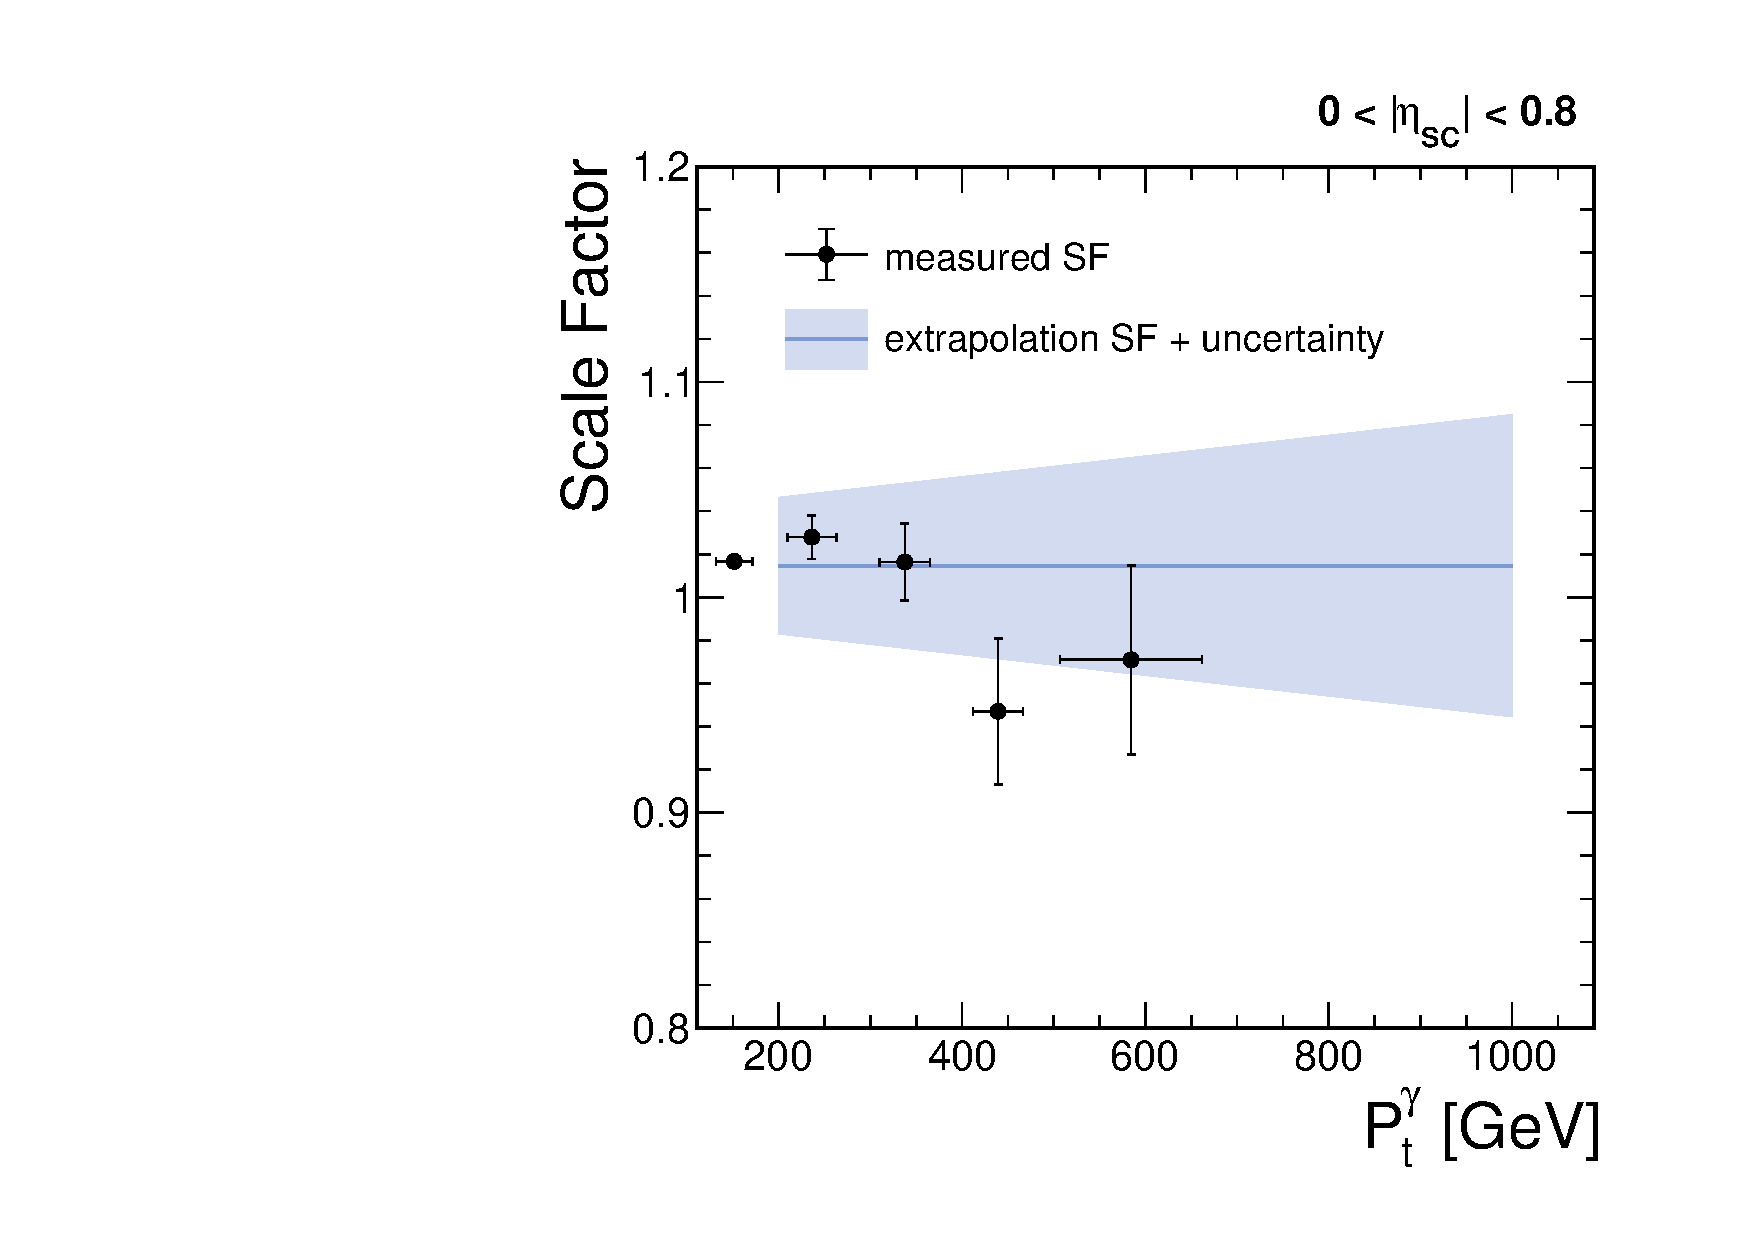
\includegraphics[width=0.3\textwidth]{fig/Extrapolate_2017_0_Check.pdf}
  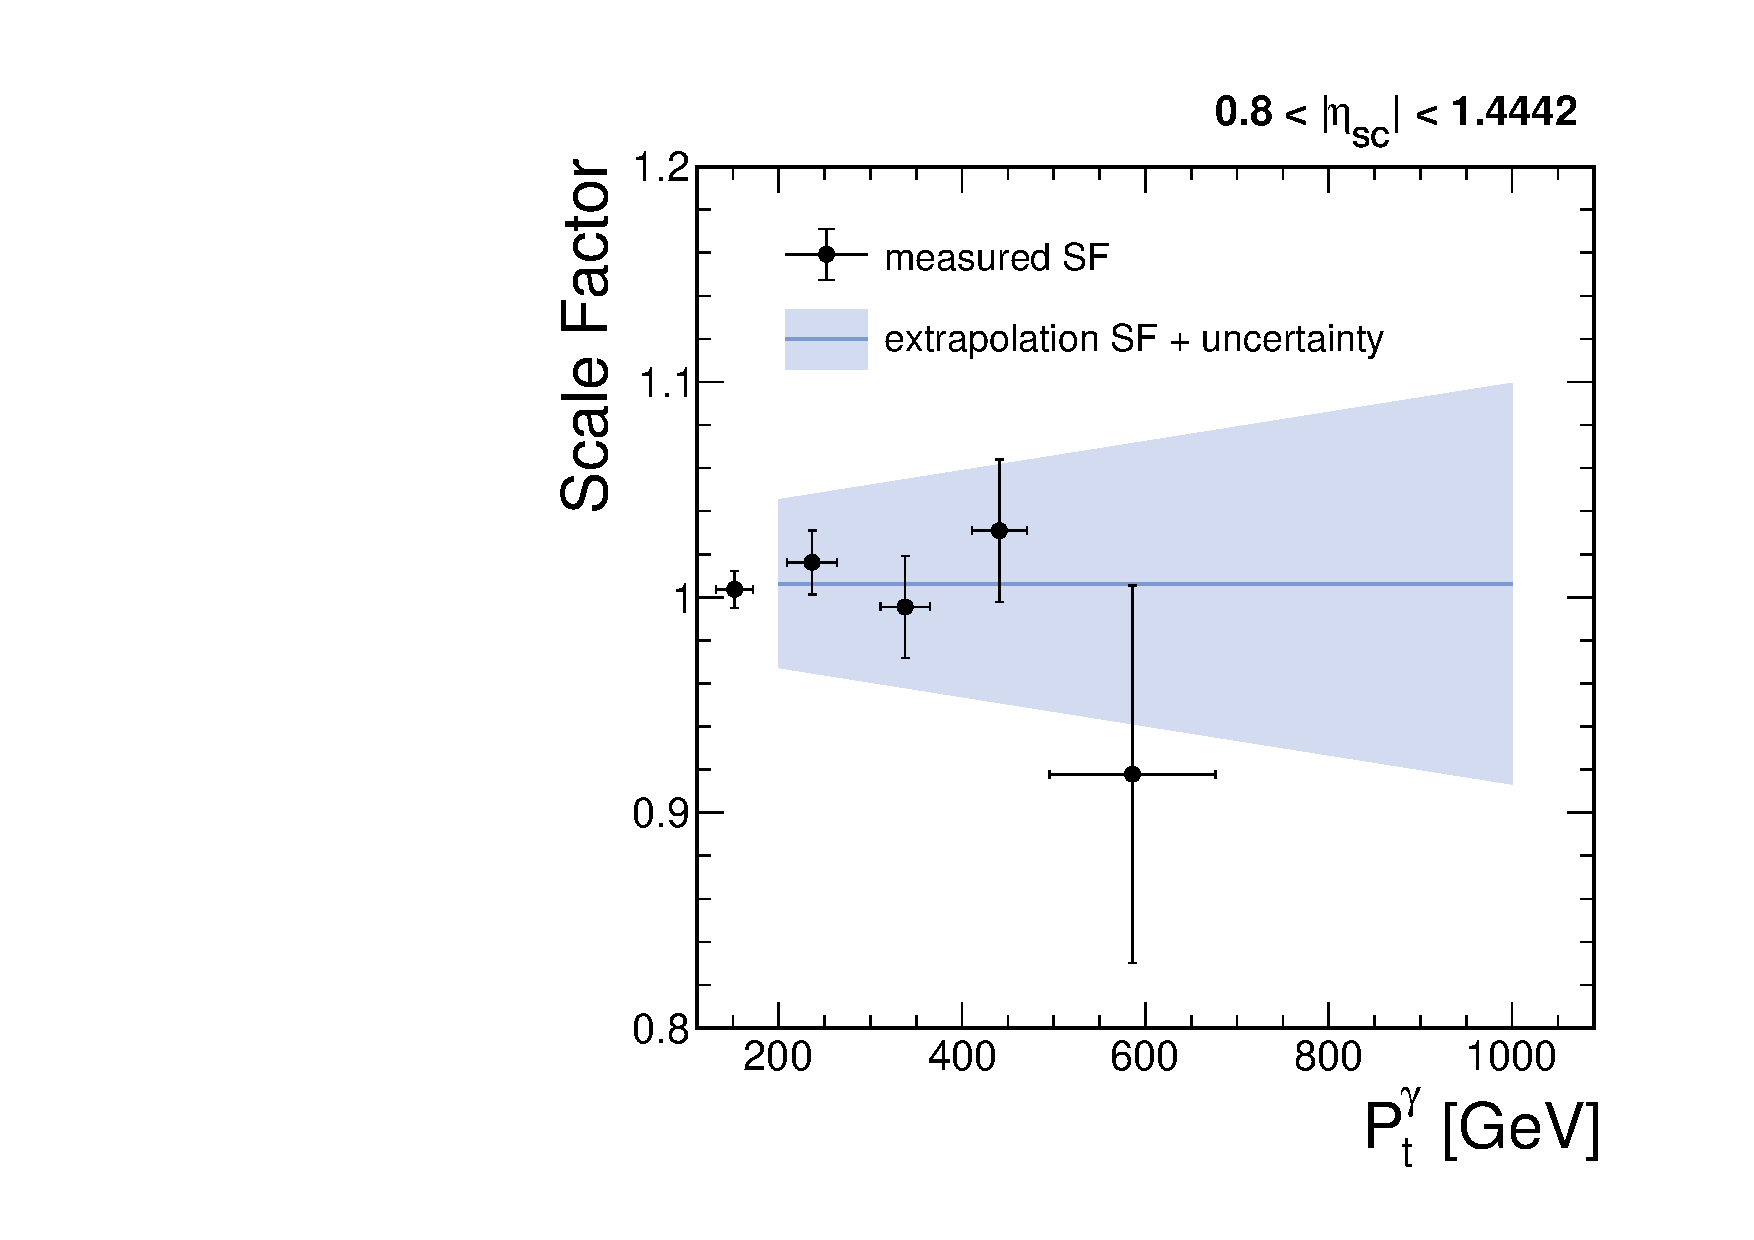
\includegraphics[width=0.3\textwidth]{fig/Extrapolate_2017_1_Check.pdf}
  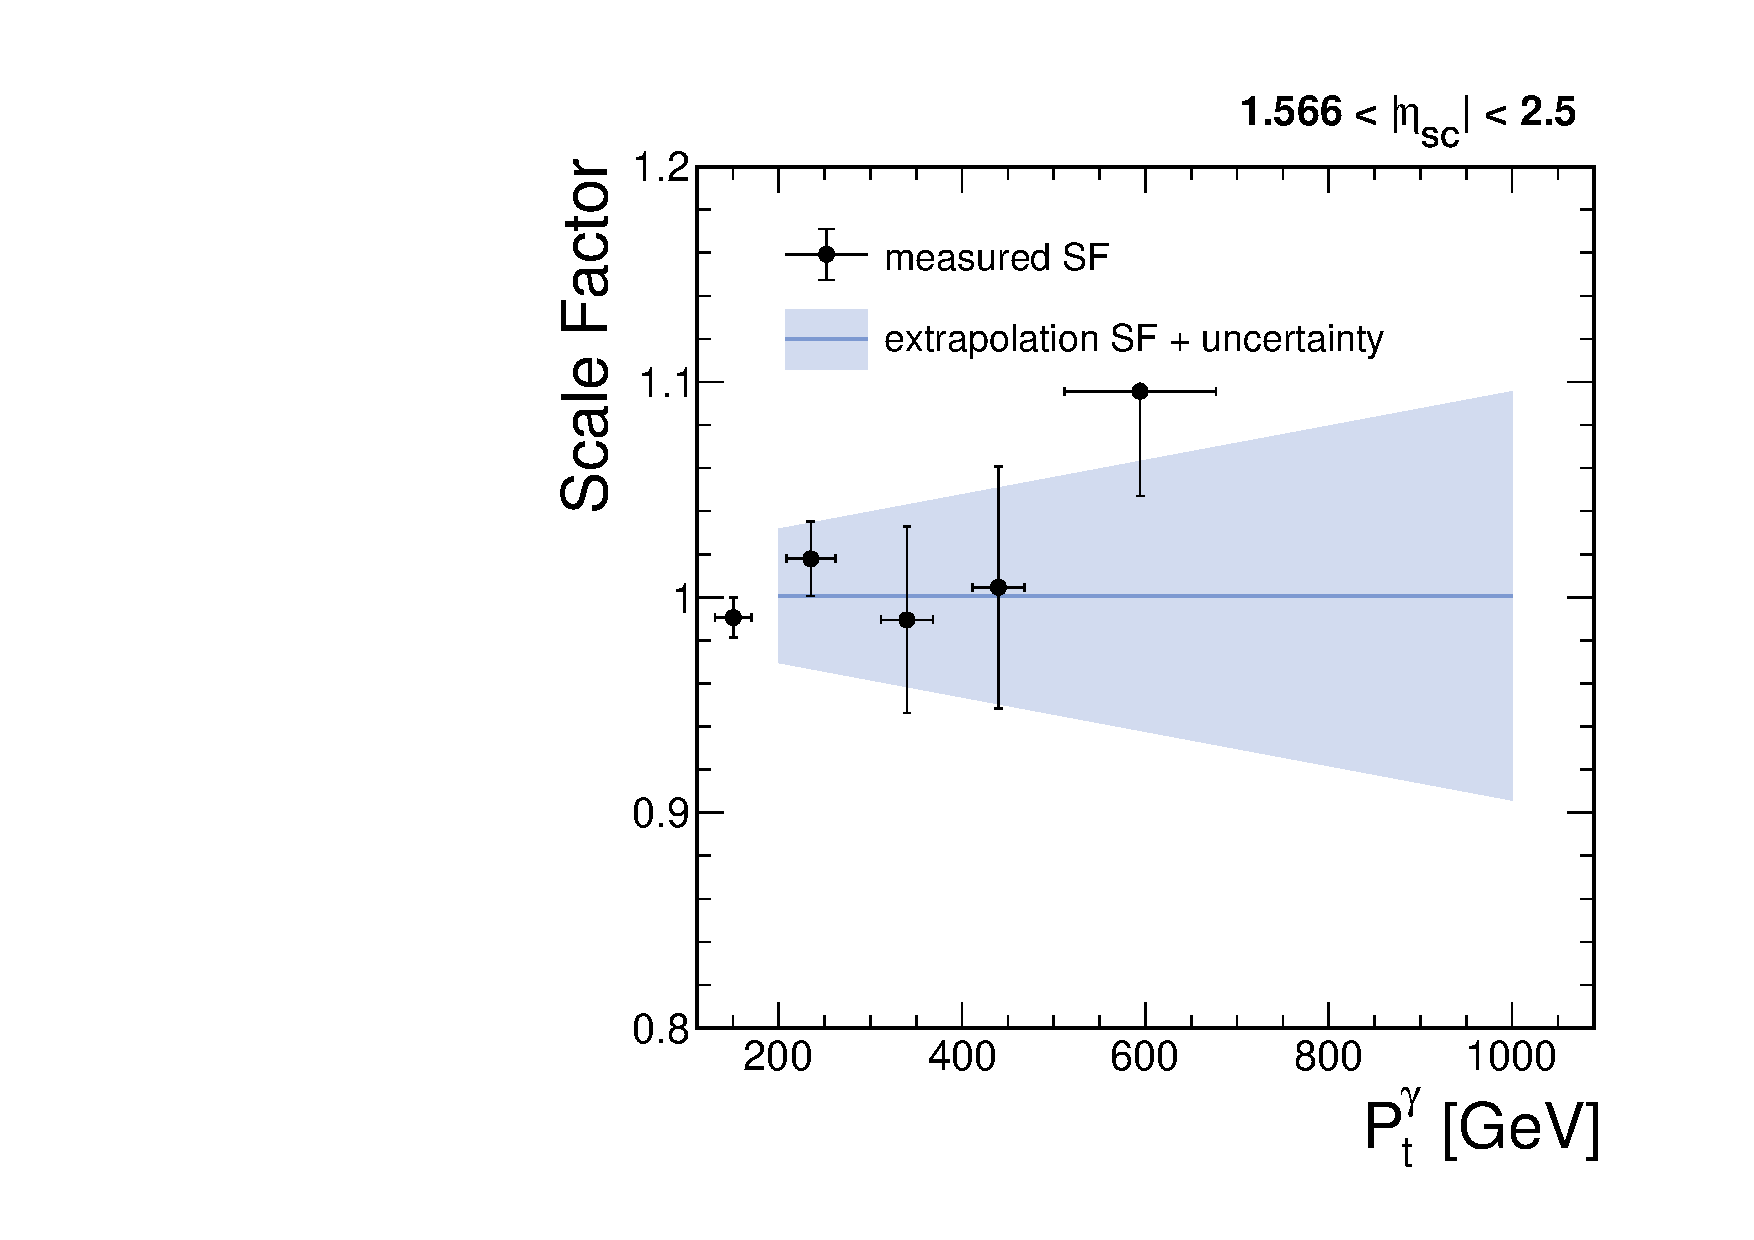
\includegraphics[width=0.3\textwidth]{fig/Extrapolate_2017_2_Check.pdf}\\
  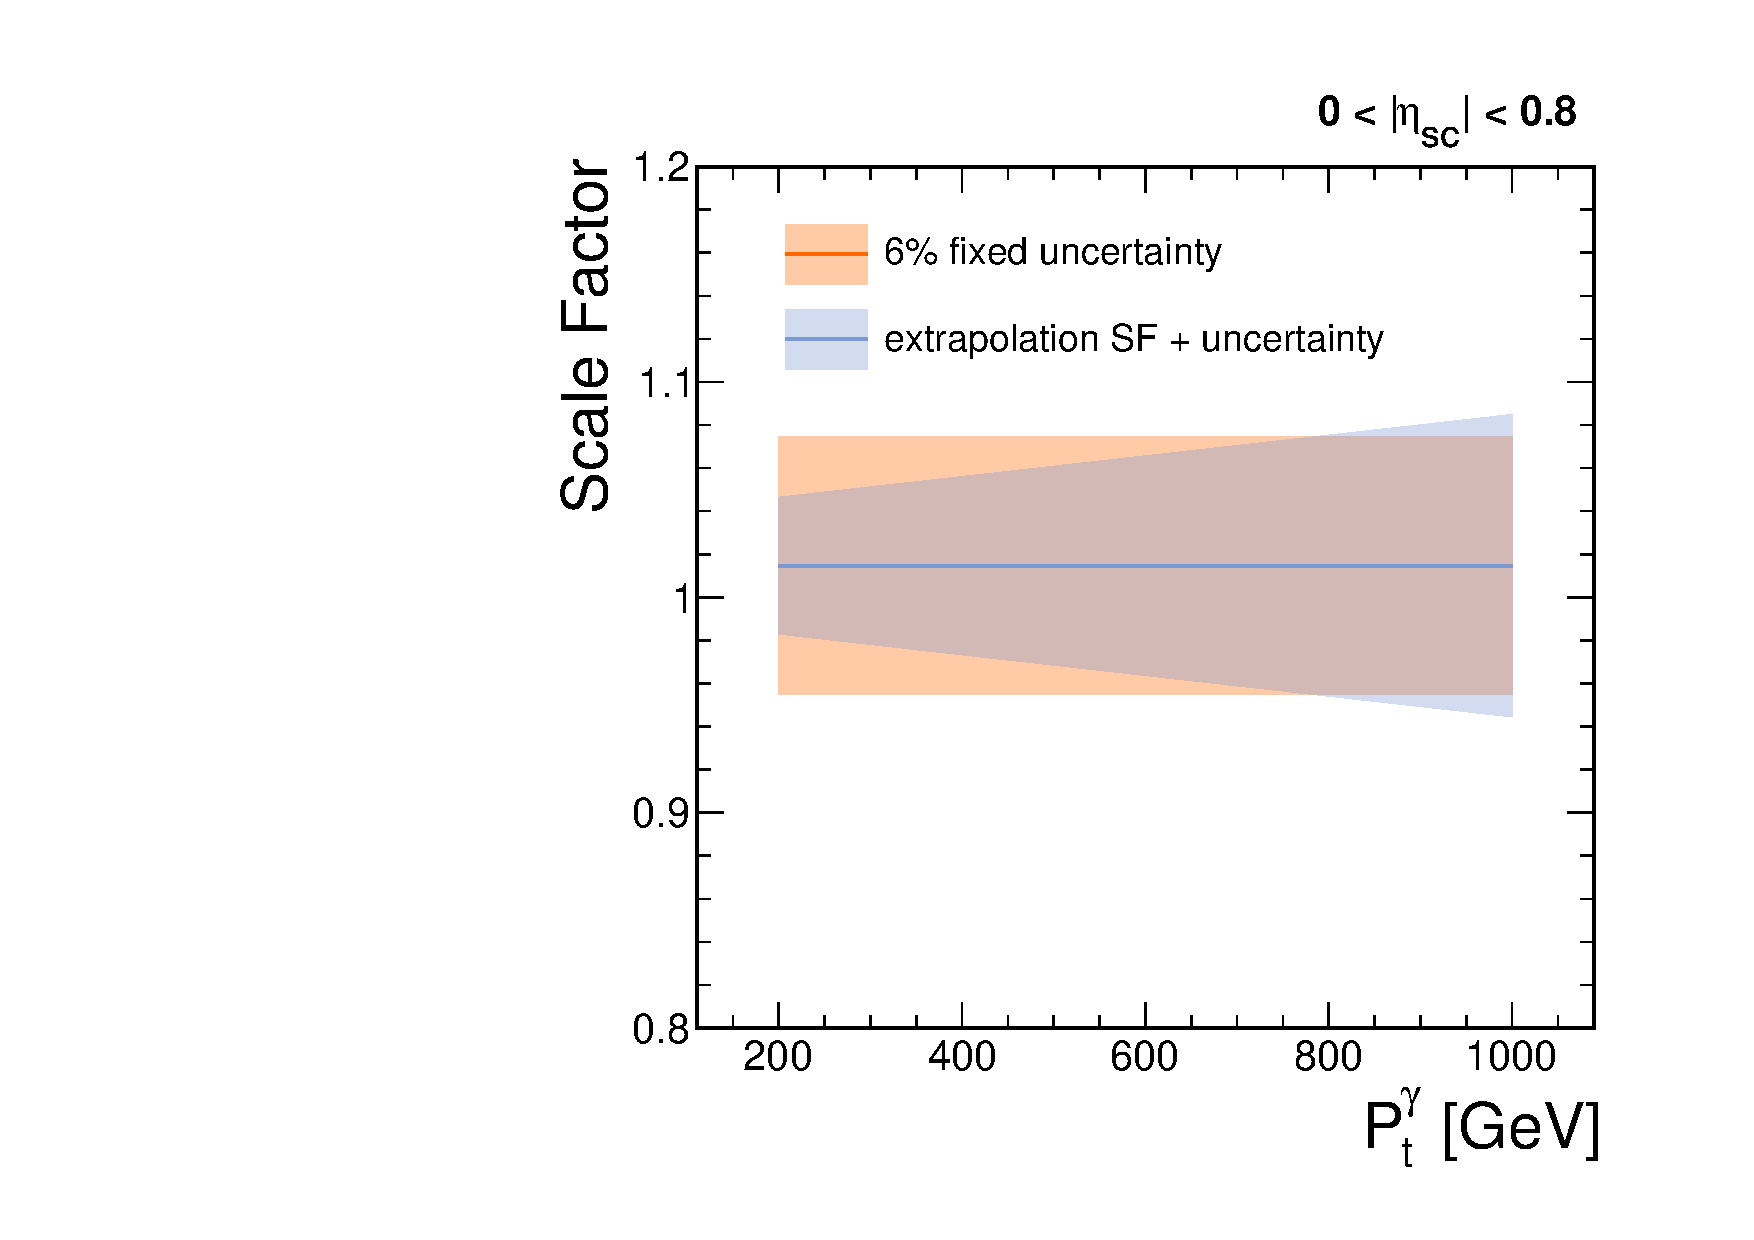
\includegraphics[width=0.3\textwidth]{fig/Extrapolate_2017_0_Compare.pdf}
  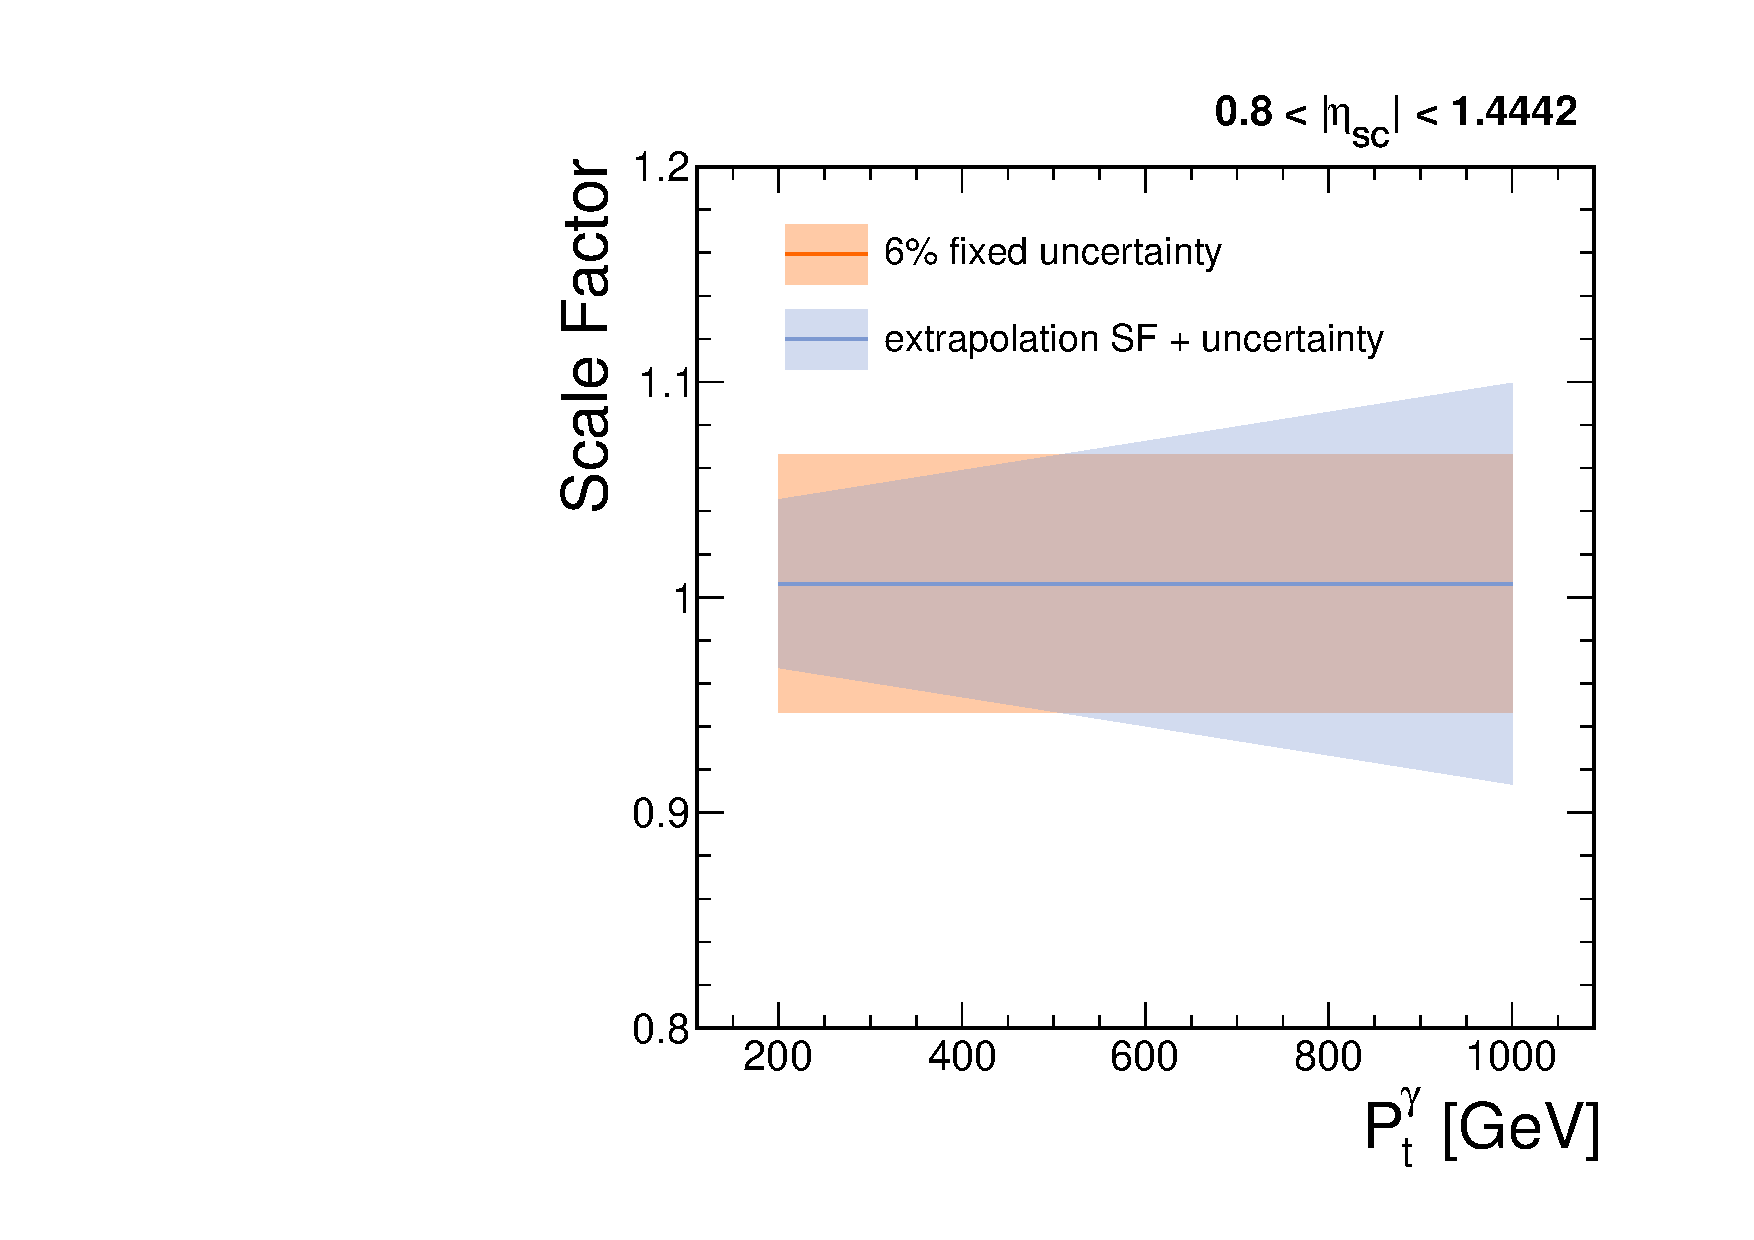
\includegraphics[width=0.3\textwidth]{fig/Extrapolate_2017_1_Compare.pdf}
  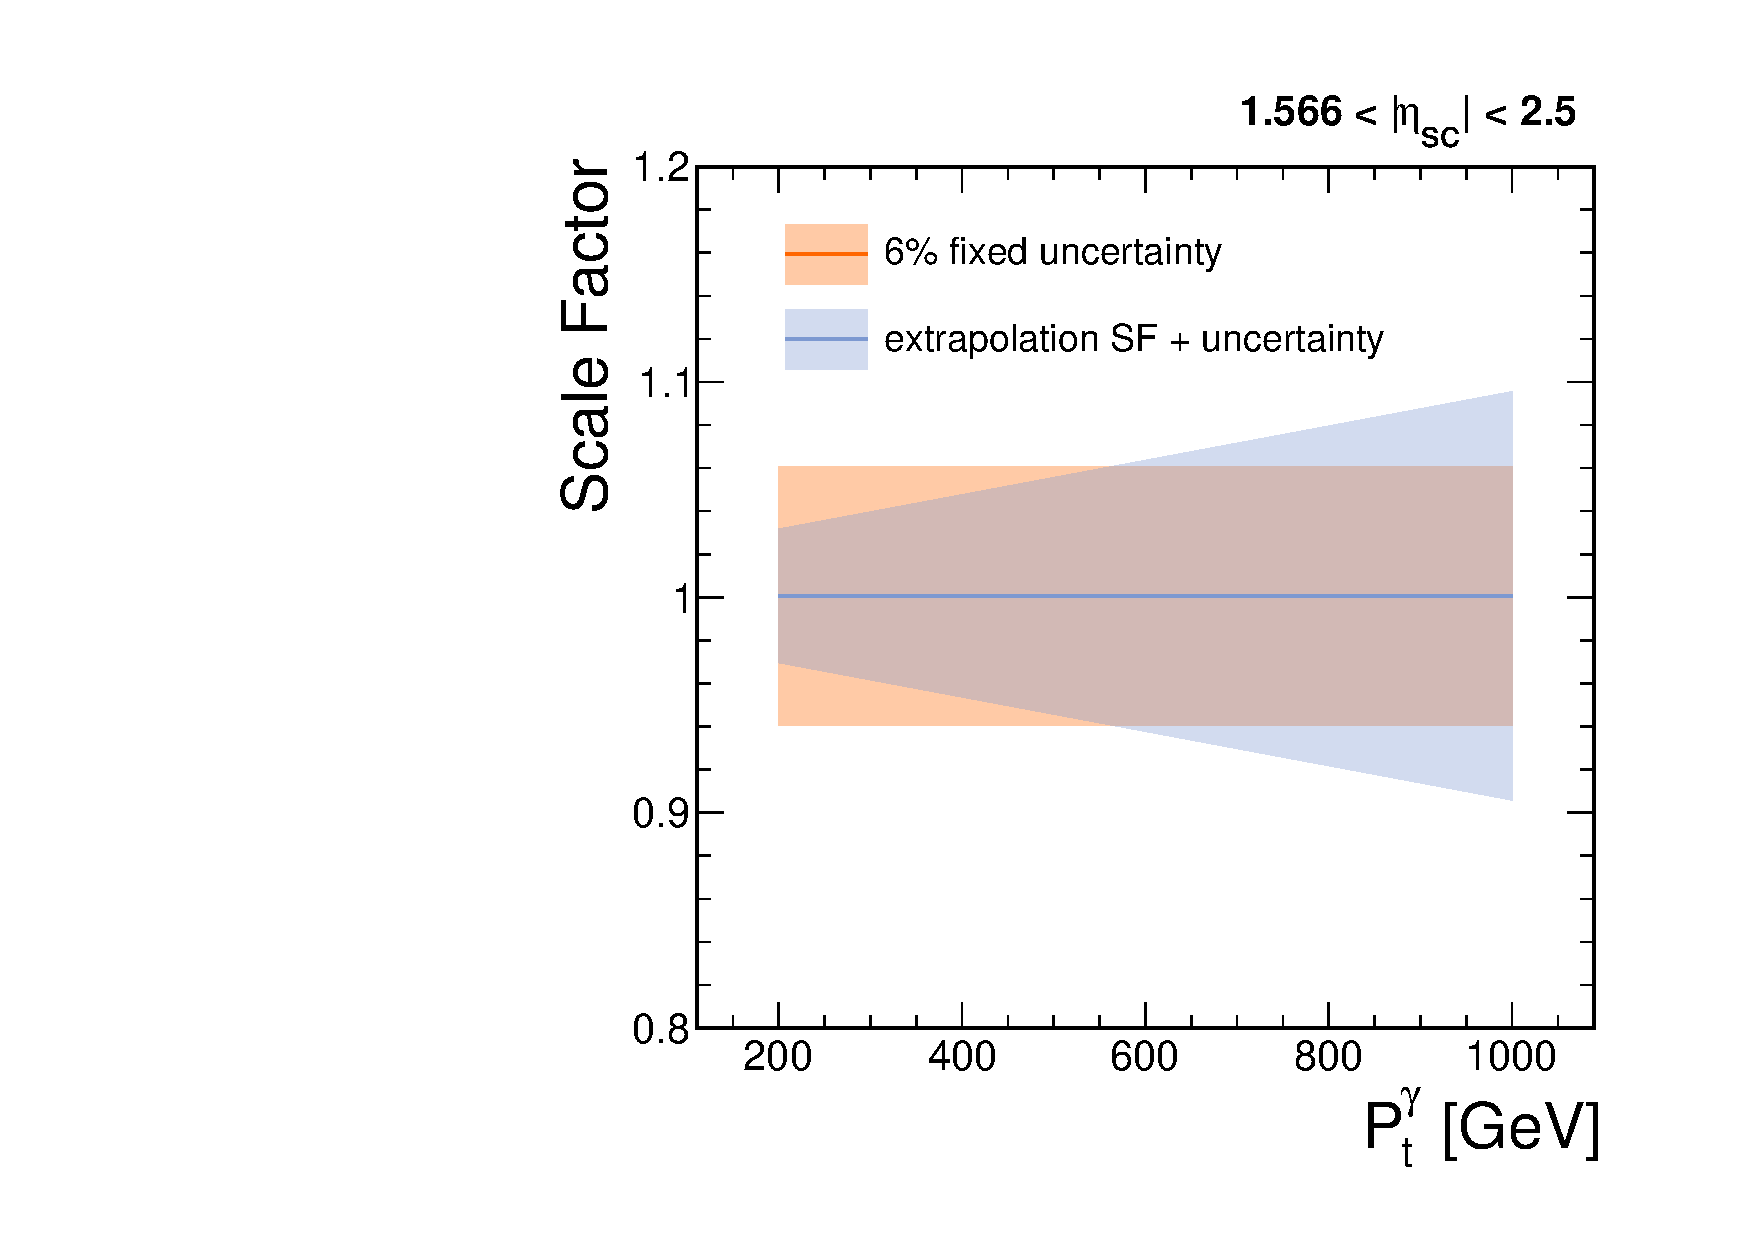
\includegraphics[width=0.3\textwidth]{fig/Extrapolate_2017_2_Compare.pdf}
 
  \label{fig:Extrapolation2017}
\end{figure}

\begin{figure}[!htbp]
  \centering
   \caption{Extrapolation plots for 2018. (a,b,c) are the extrapolation fitting results. (d,e,f) are consistency checks. The extrapolated scale factors and uncertainties are drawn on top of the tag-and-probe measured results.}
  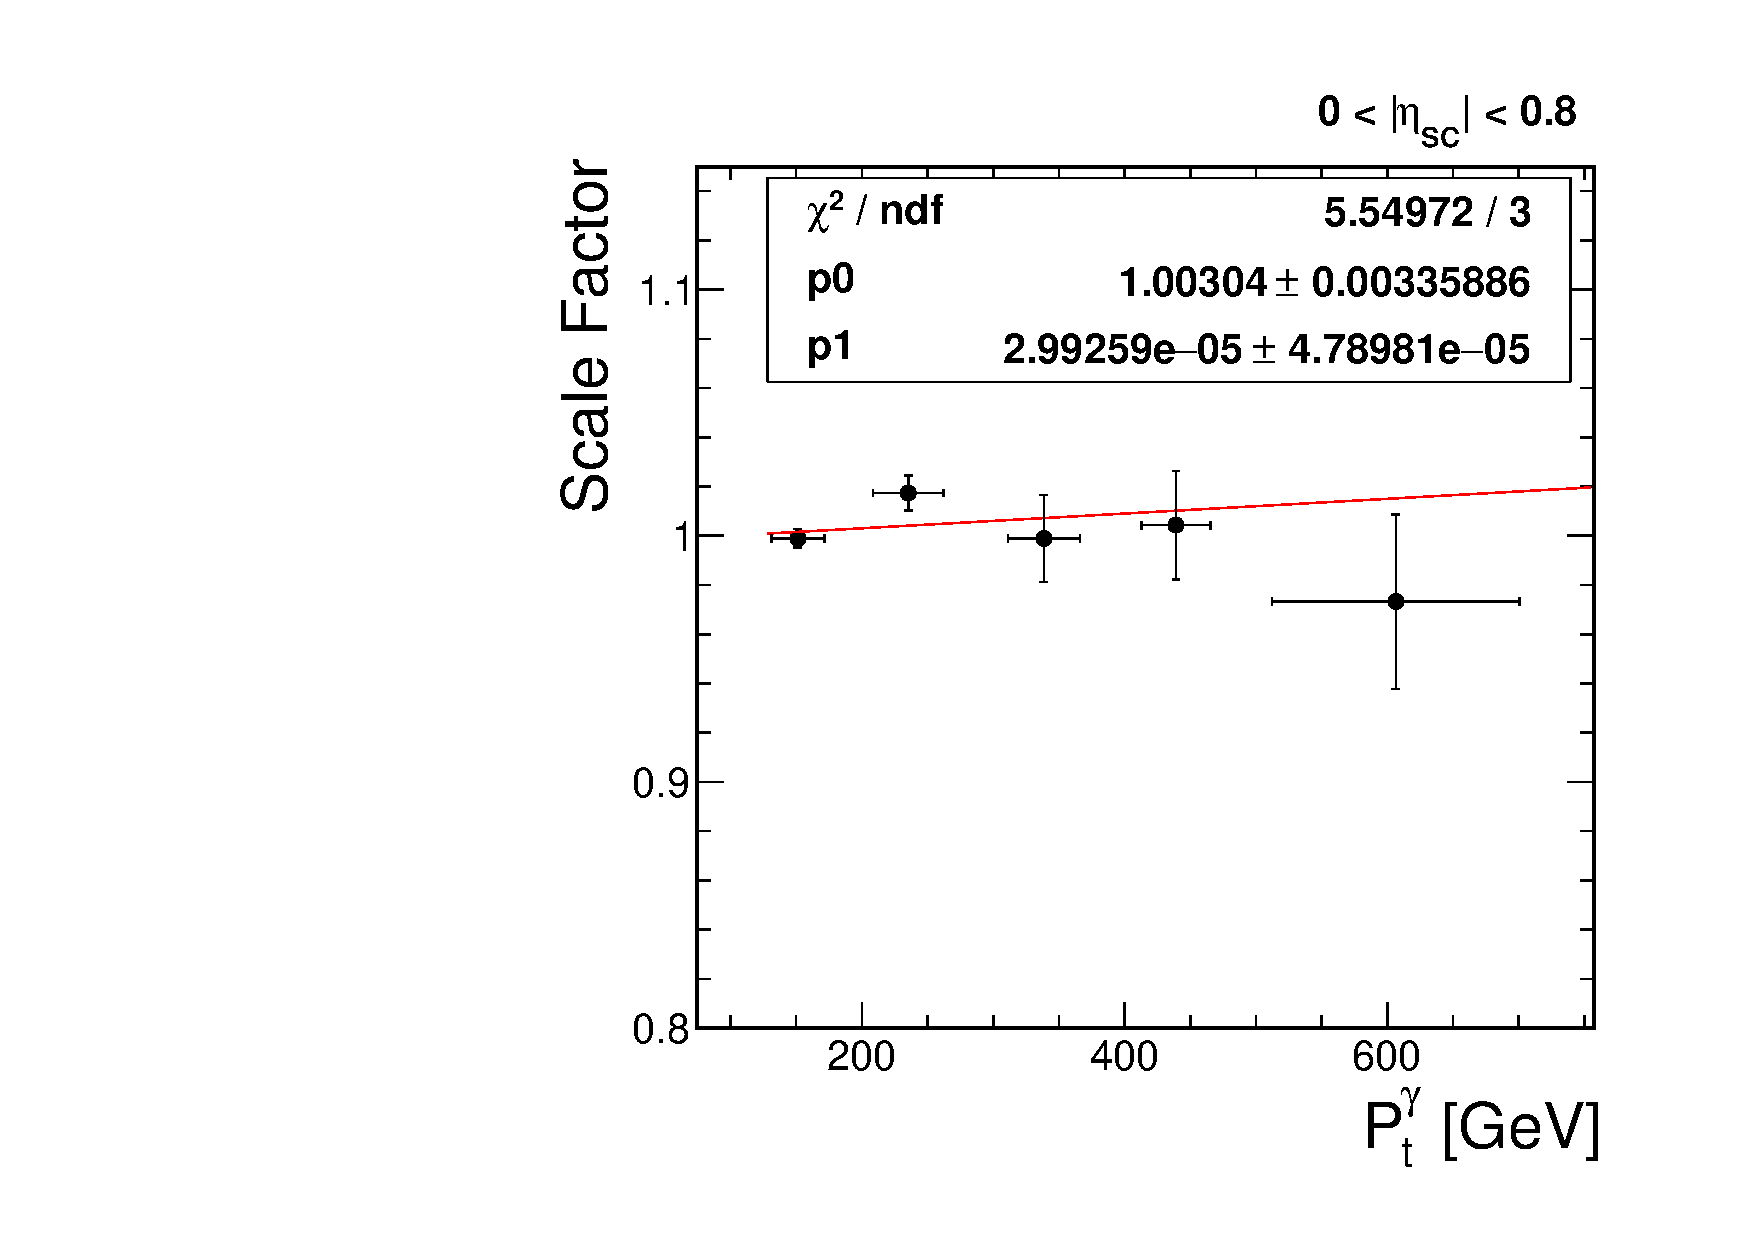
\includegraphics[width=0.3\textwidth]{fig/Extrapolate_2018_0_Fit.pdf}
  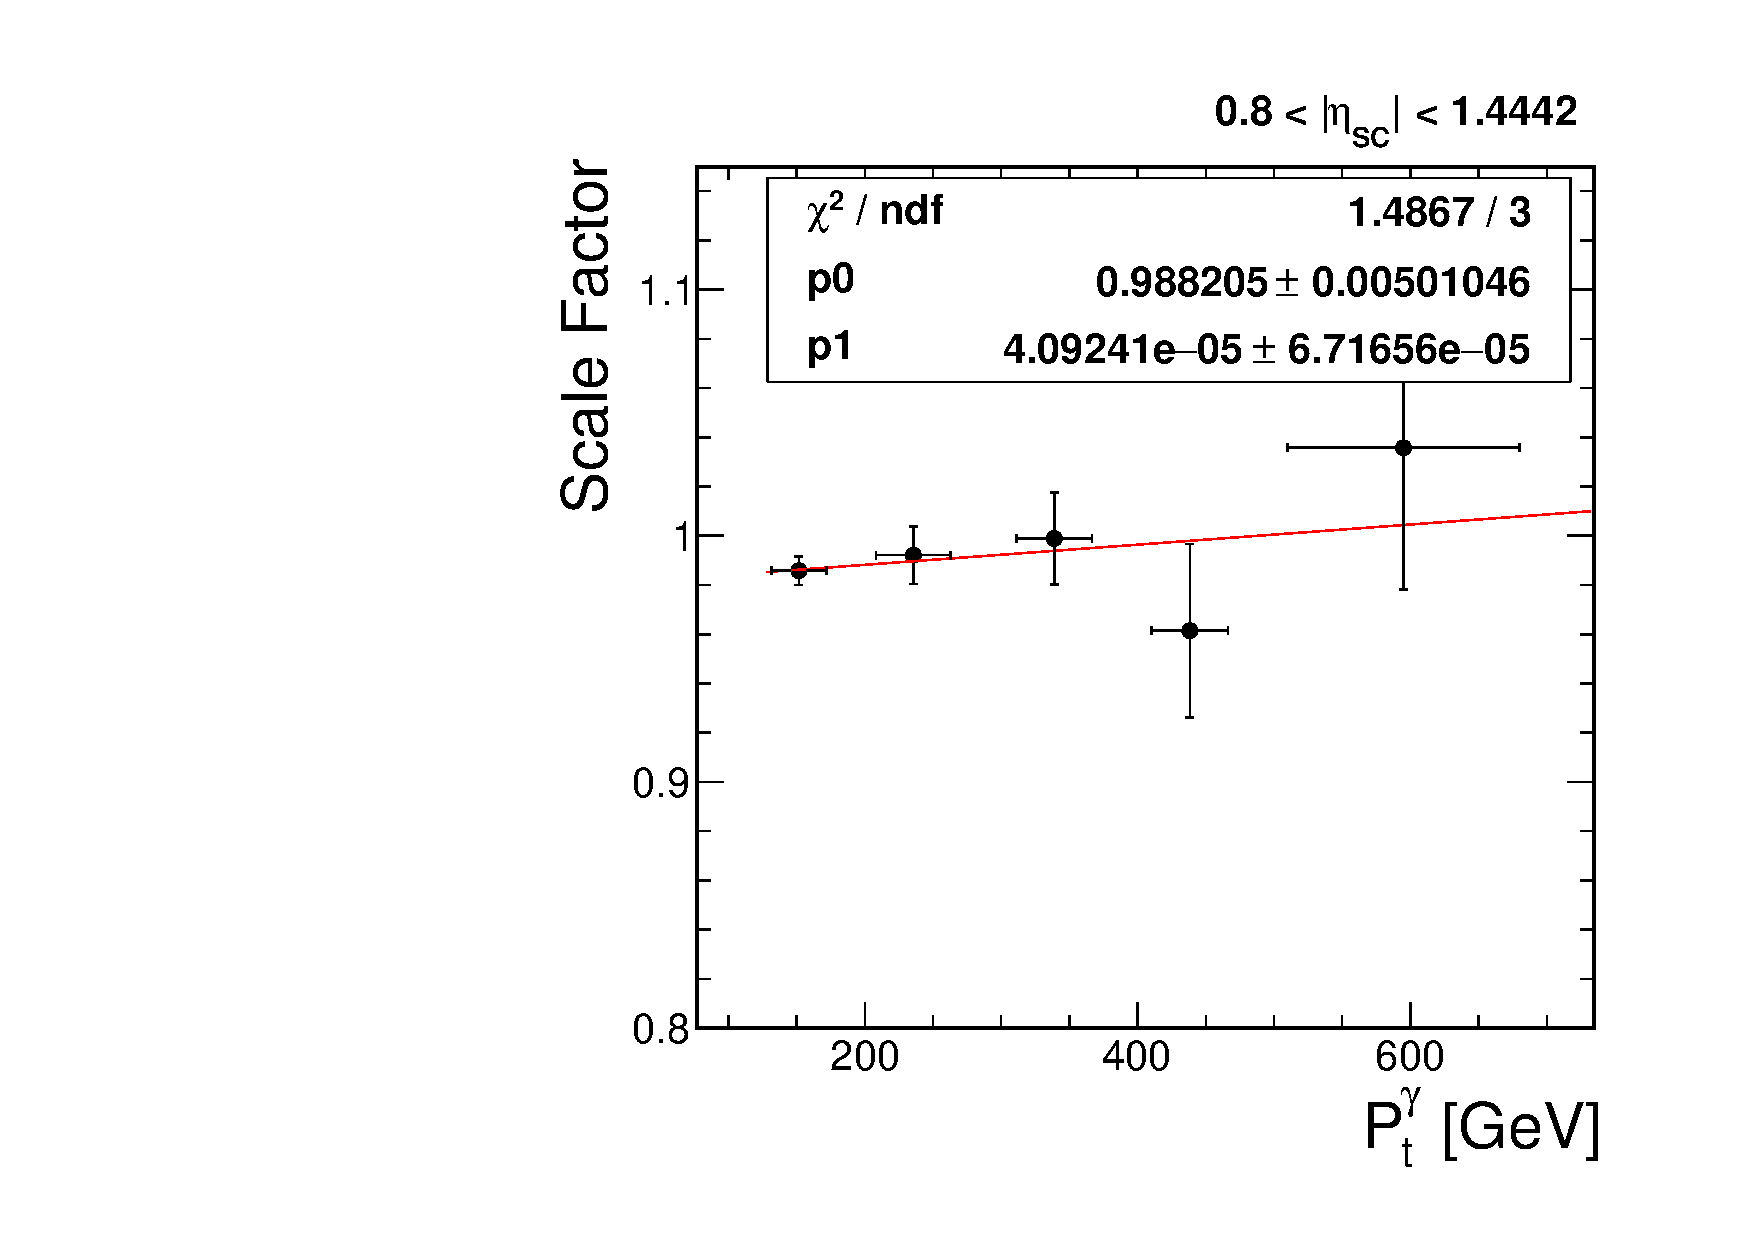
\includegraphics[width=0.3\textwidth]{fig/Extrapolate_2018_1_Fit.pdf}
  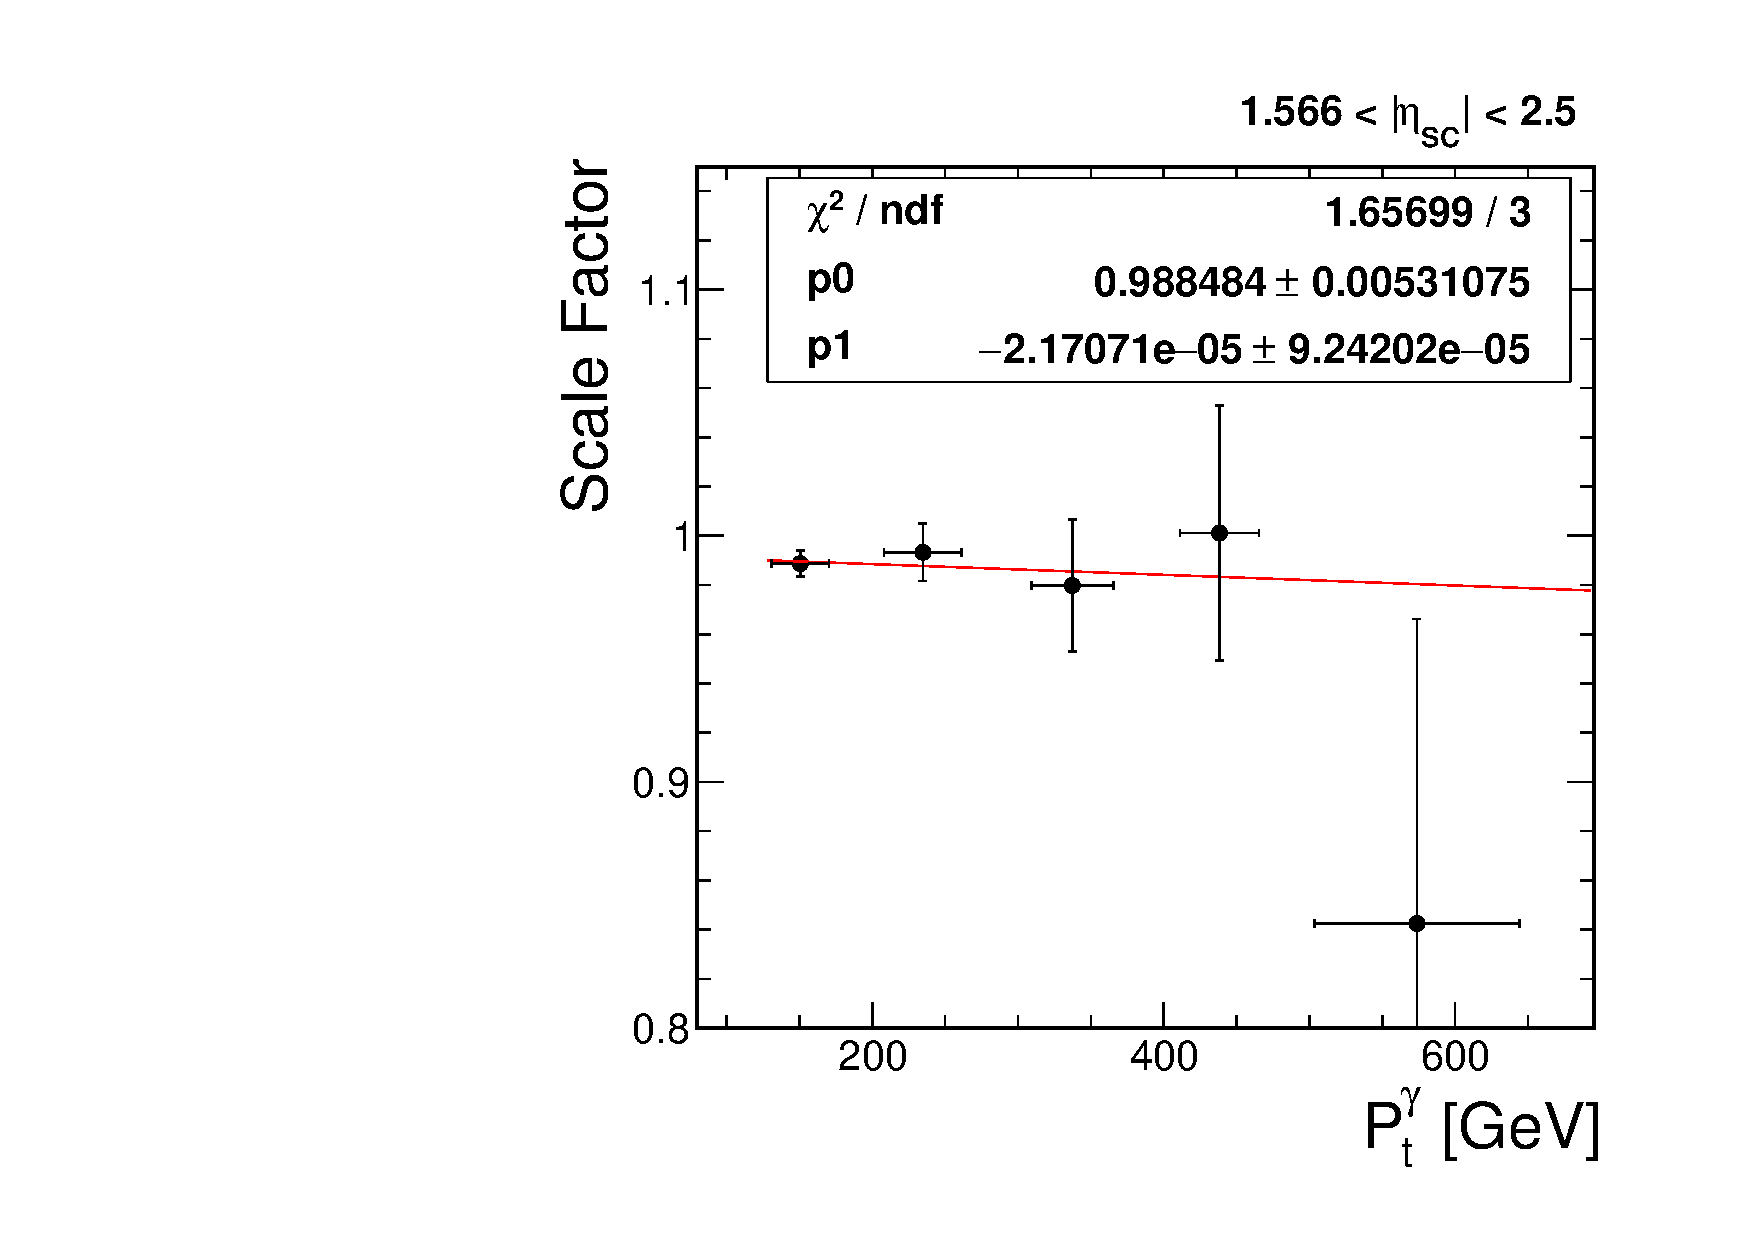
\includegraphics[width=0.3\textwidth]{fig/Extrapolate_2018_2_Fit.pdf}\\
  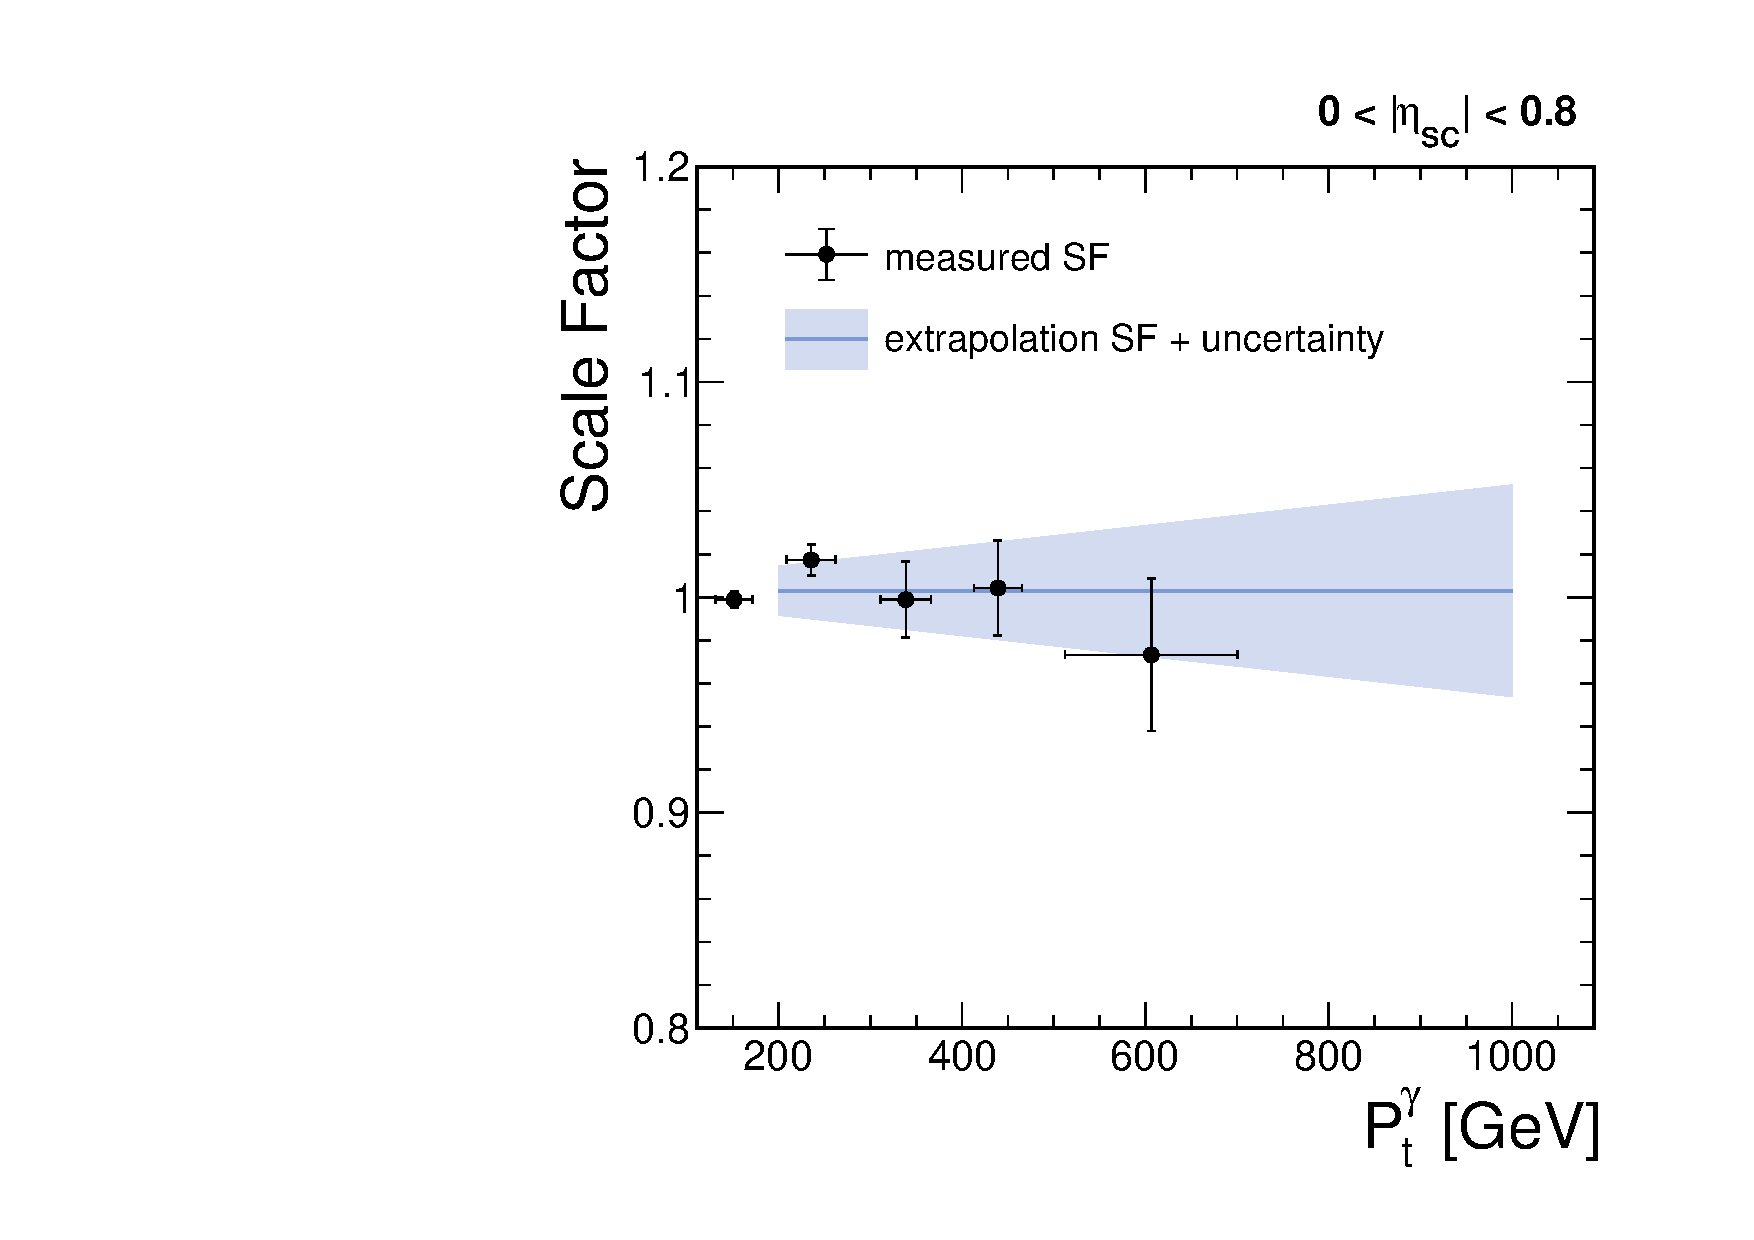
\includegraphics[width=0.3\textwidth]{fig/Extrapolate_2018_0_Check.pdf}
  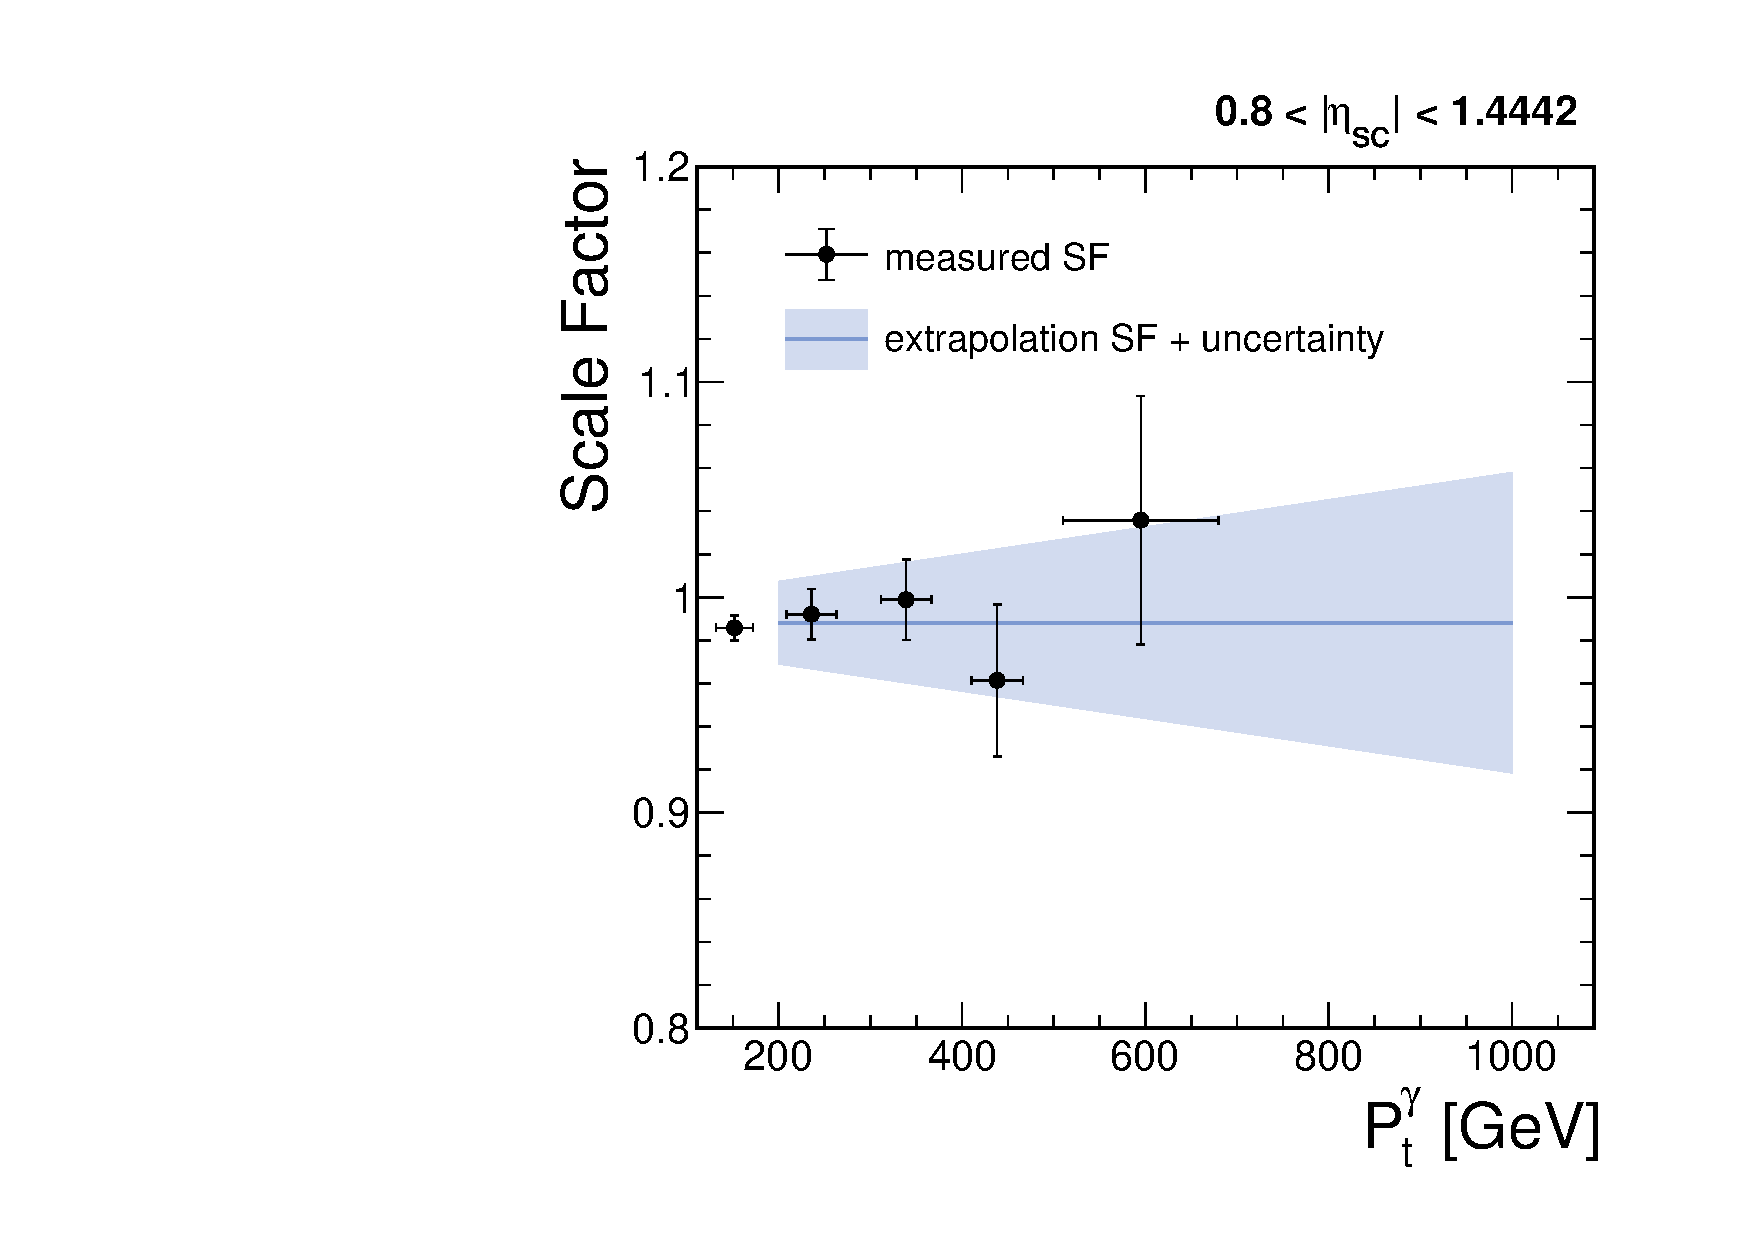
\includegraphics[width=0.3\textwidth]{fig/Extrapolate_2018_1_Check.pdf}
  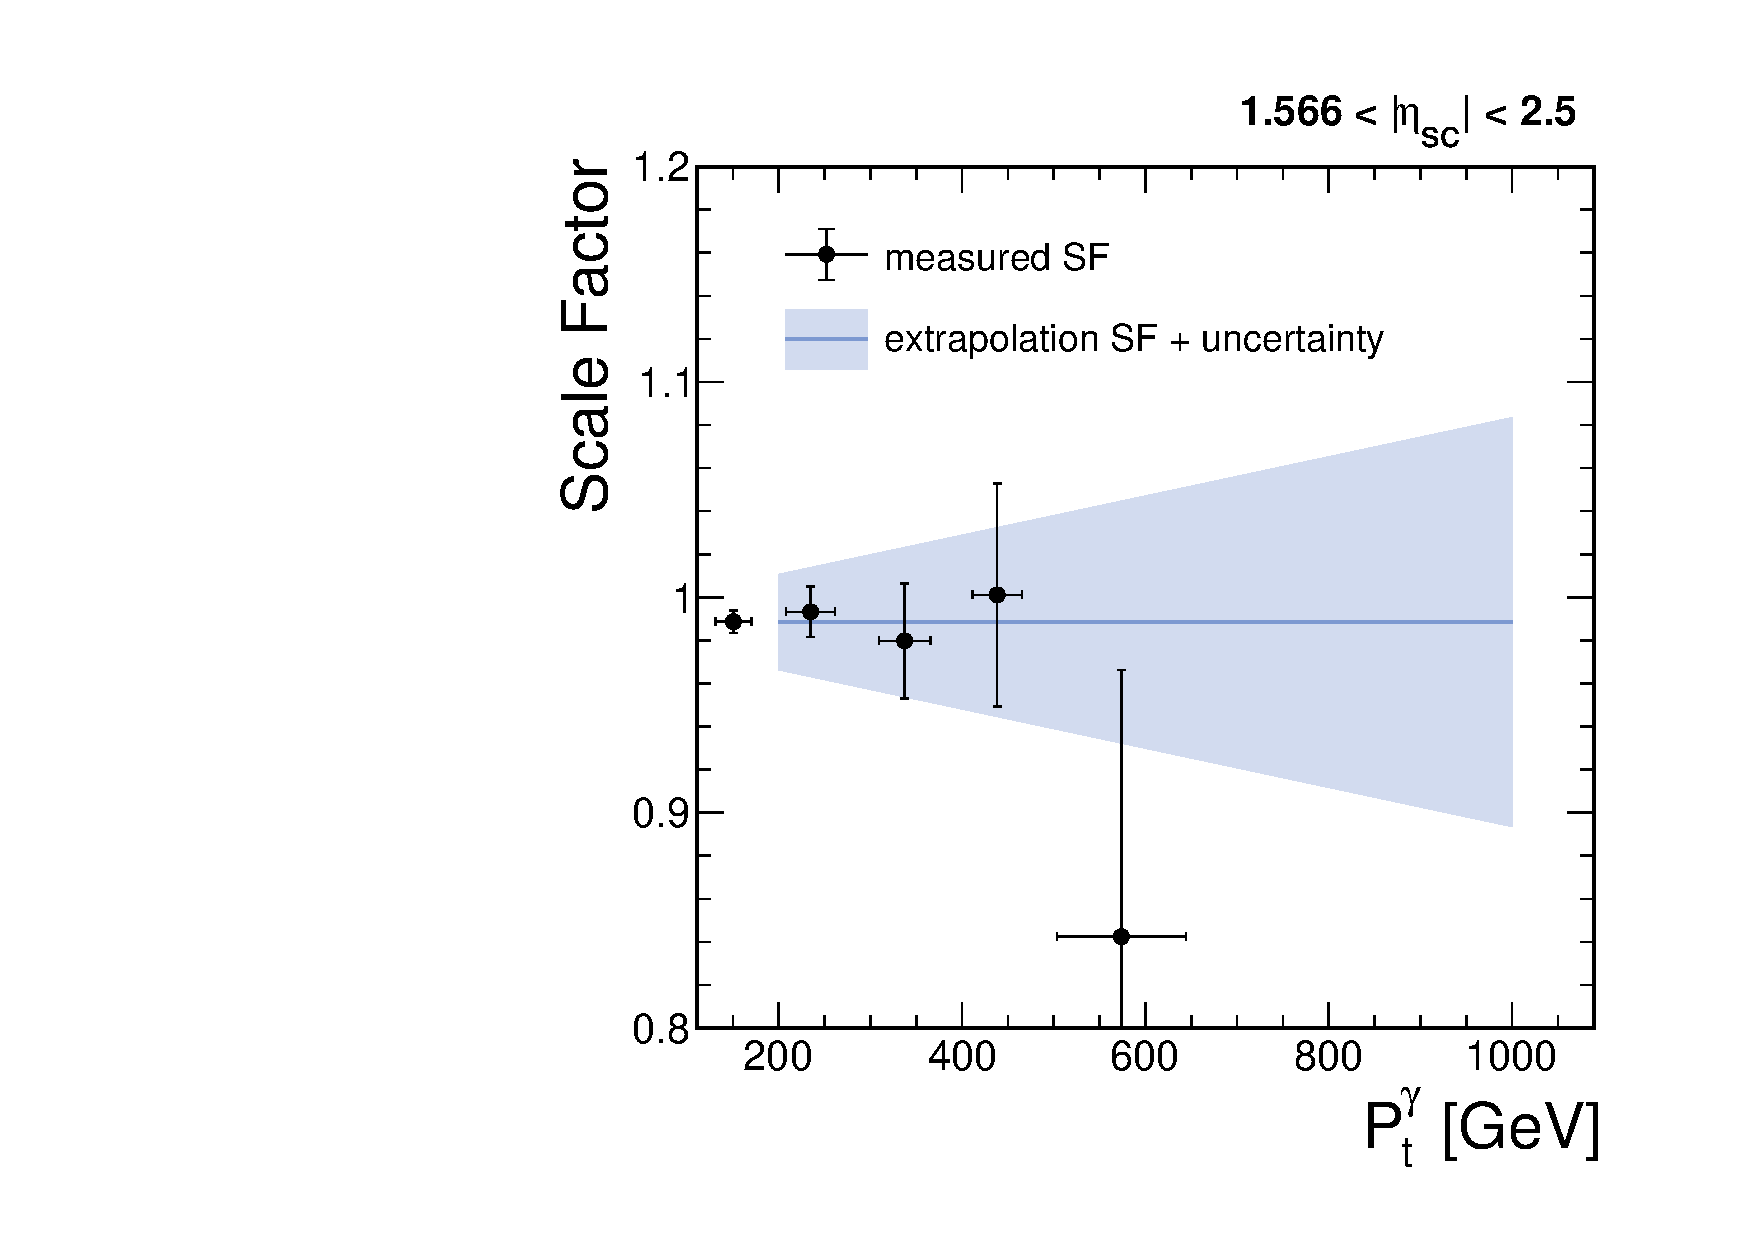
\includegraphics[width=0.3\textwidth]{fig/Extrapolate_2018_2_Check.pdf}\\
  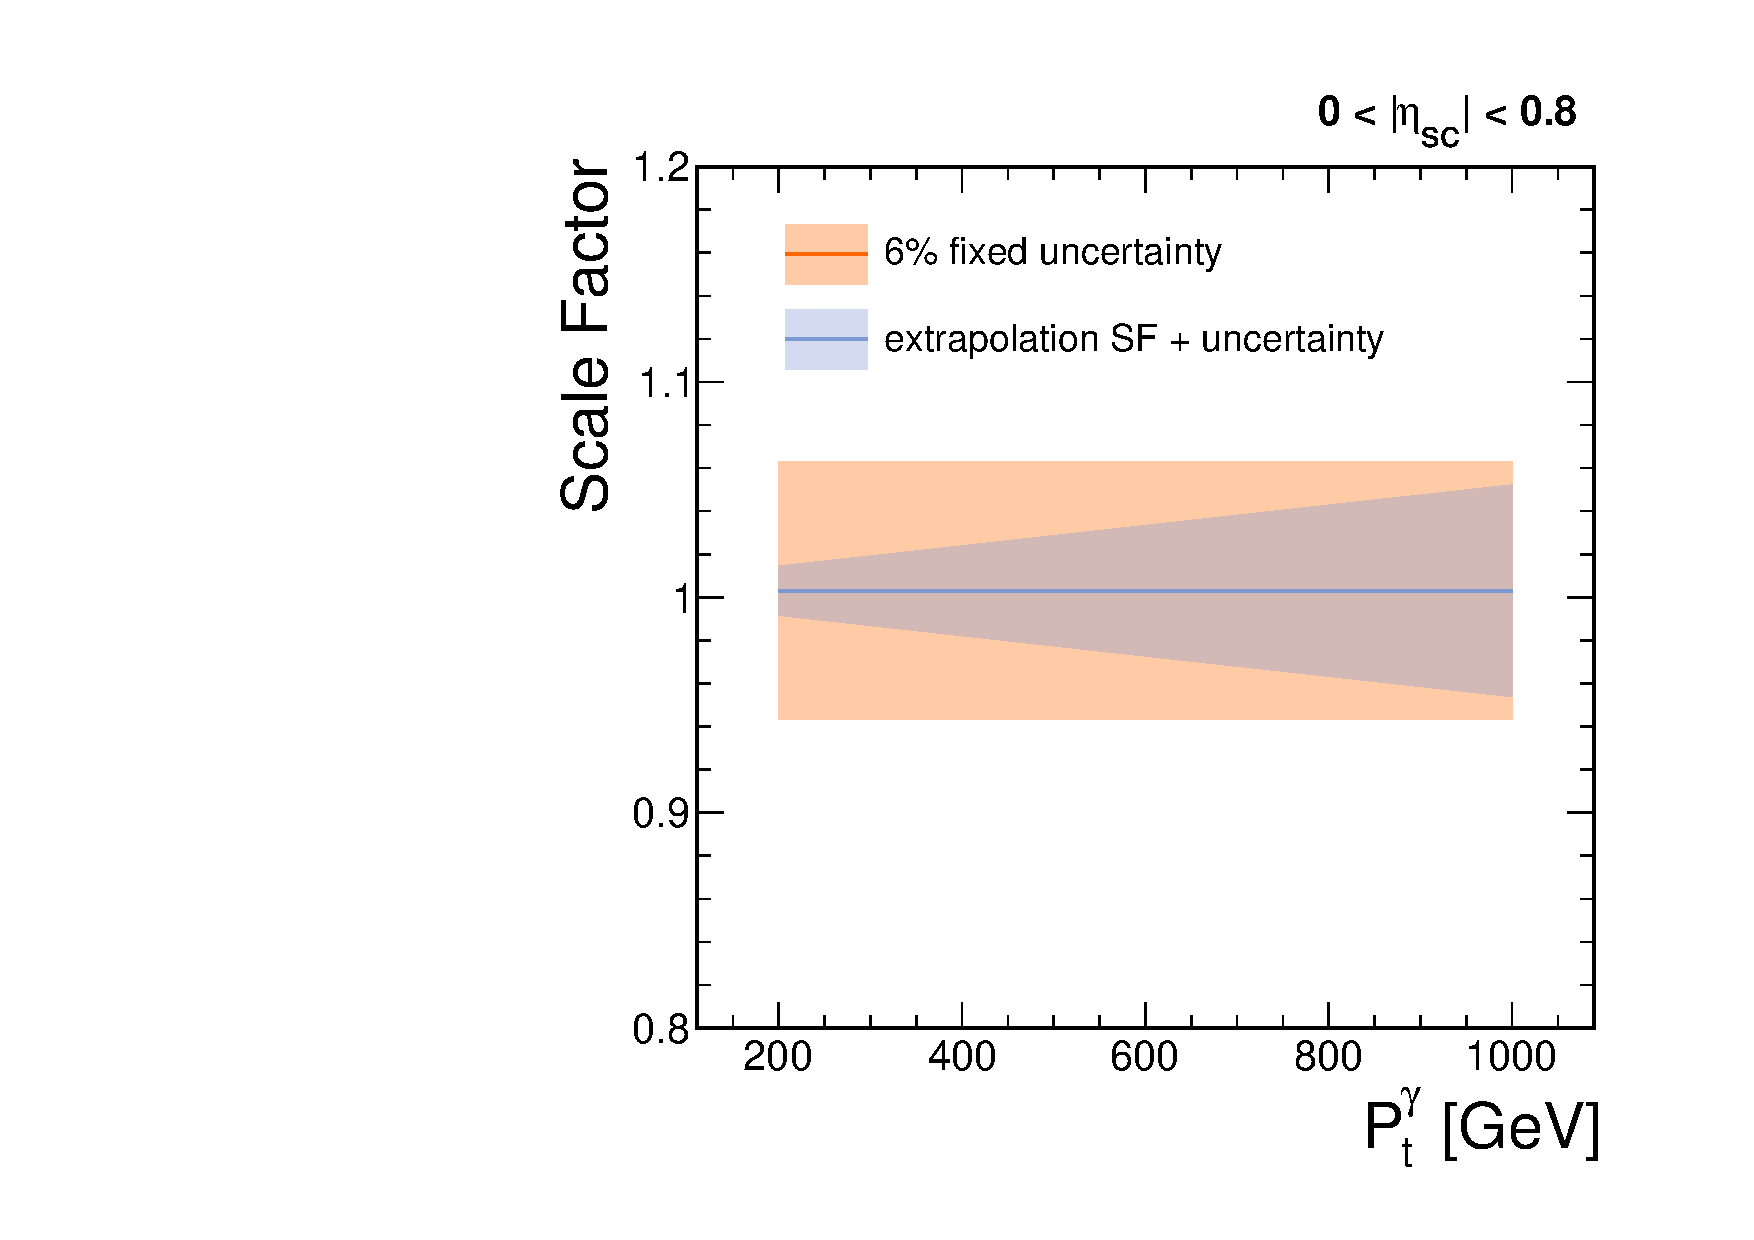
\includegraphics[width=0.3\textwidth]{fig/Extrapolate_2018_0_Compare.pdf}
  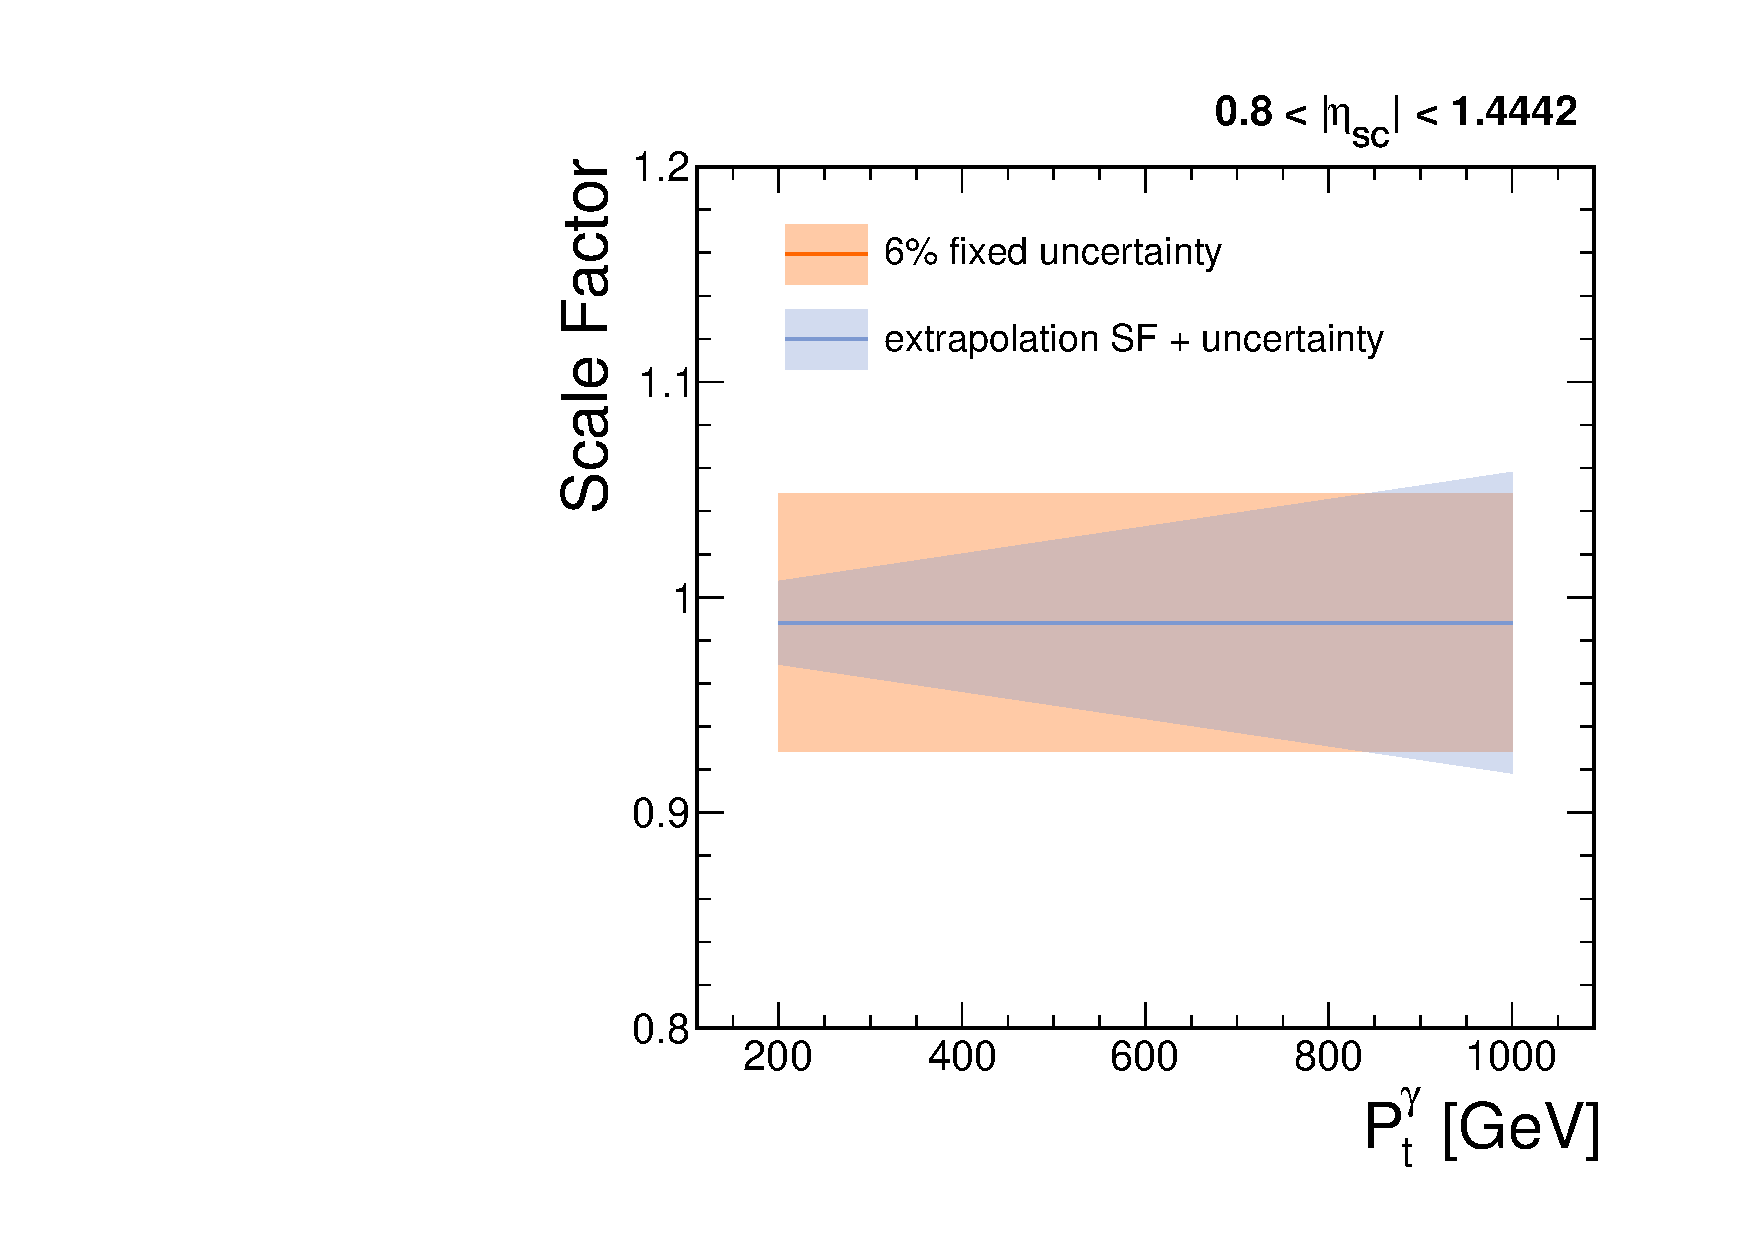
\includegraphics[width=0.3\textwidth]{fig/Extrapolate_2018_1_Compare.pdf}
  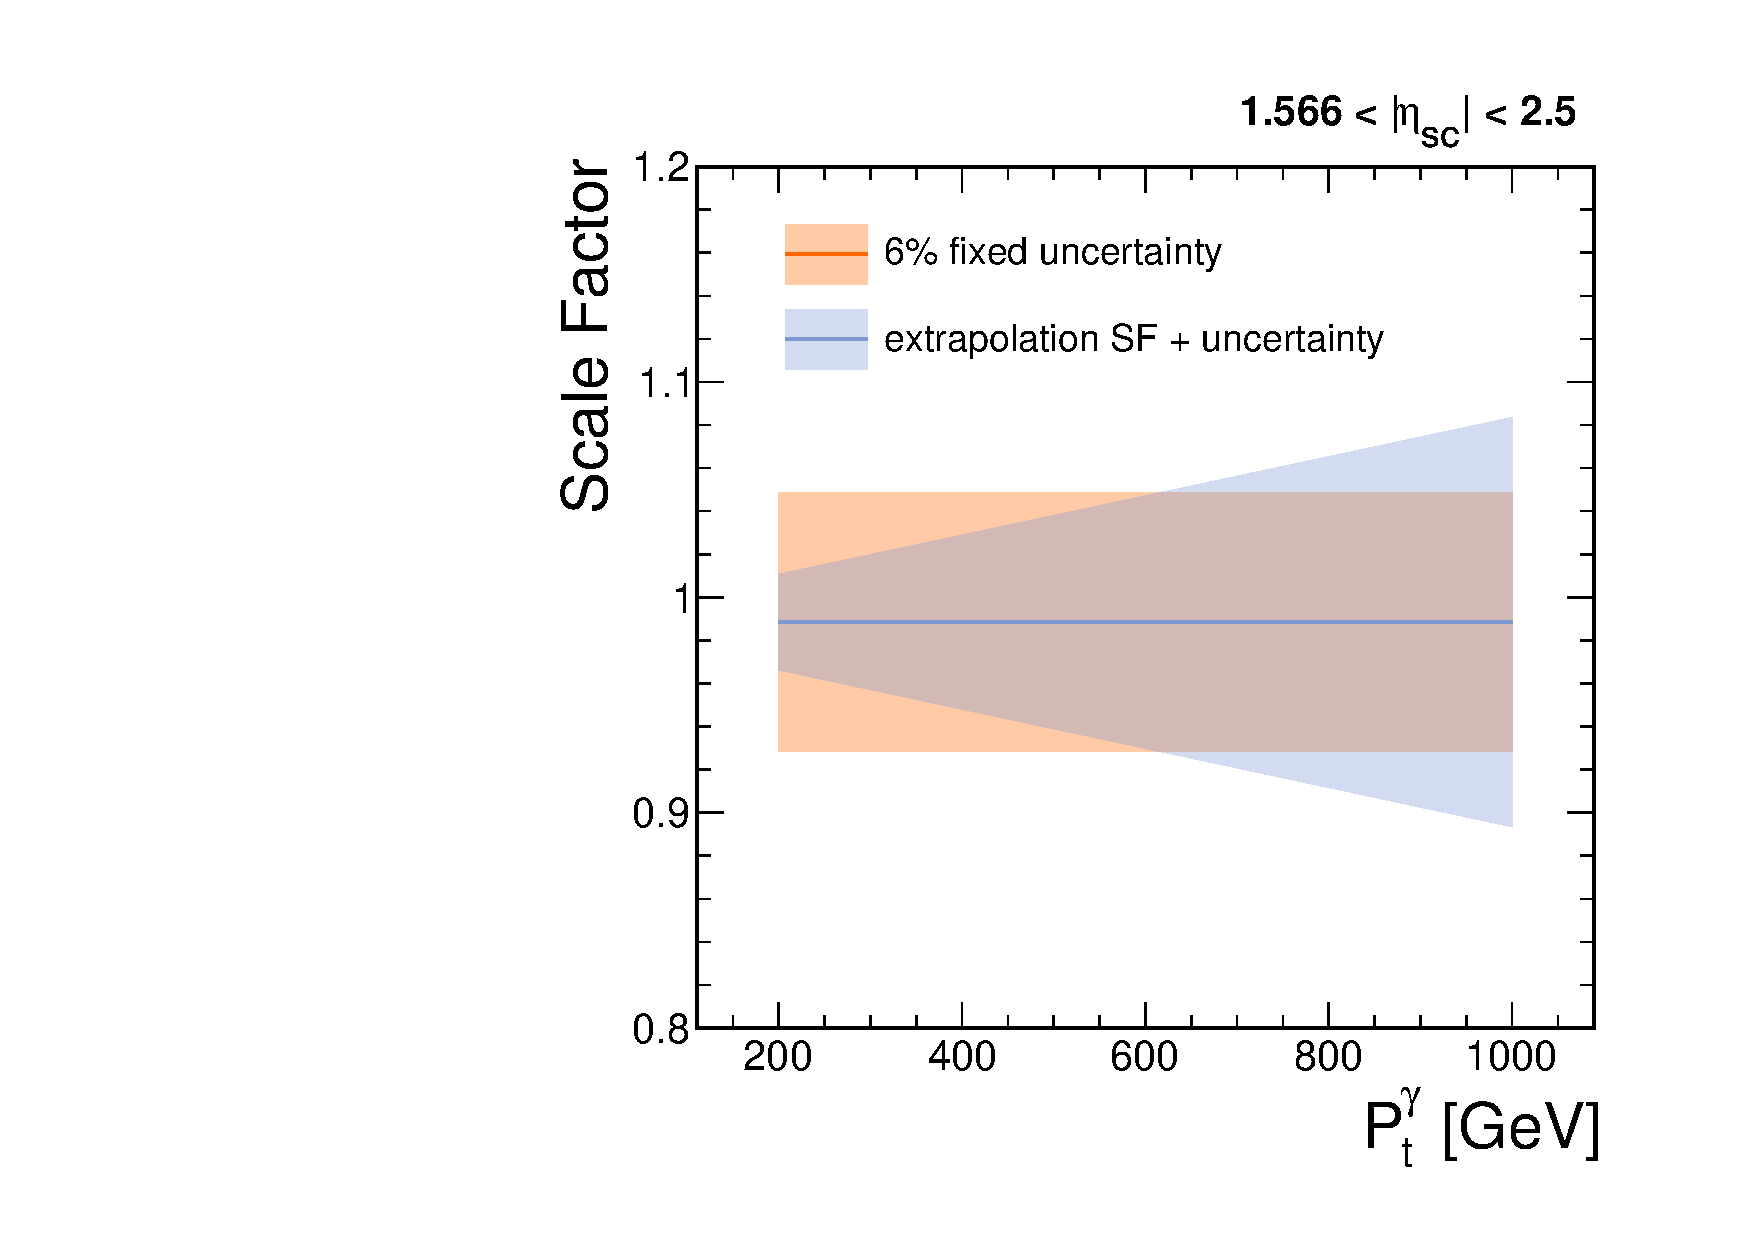
\includegraphics[width=0.3\textwidth]{fig/Extrapolate_2018_2_Compare.pdf}
 
  \label{fig:Extrapolation2018}
\end{figure}

\begin{figure}[!htbp]
\caption{Data efficiency and scale factors (bottom) extracted from the tag-and-probe package are plotted vs \pt for three years.}
\begin{center}
%\includegraphics[angle=0,width=0.4\textwidth]{figures/eff2015.pdf}
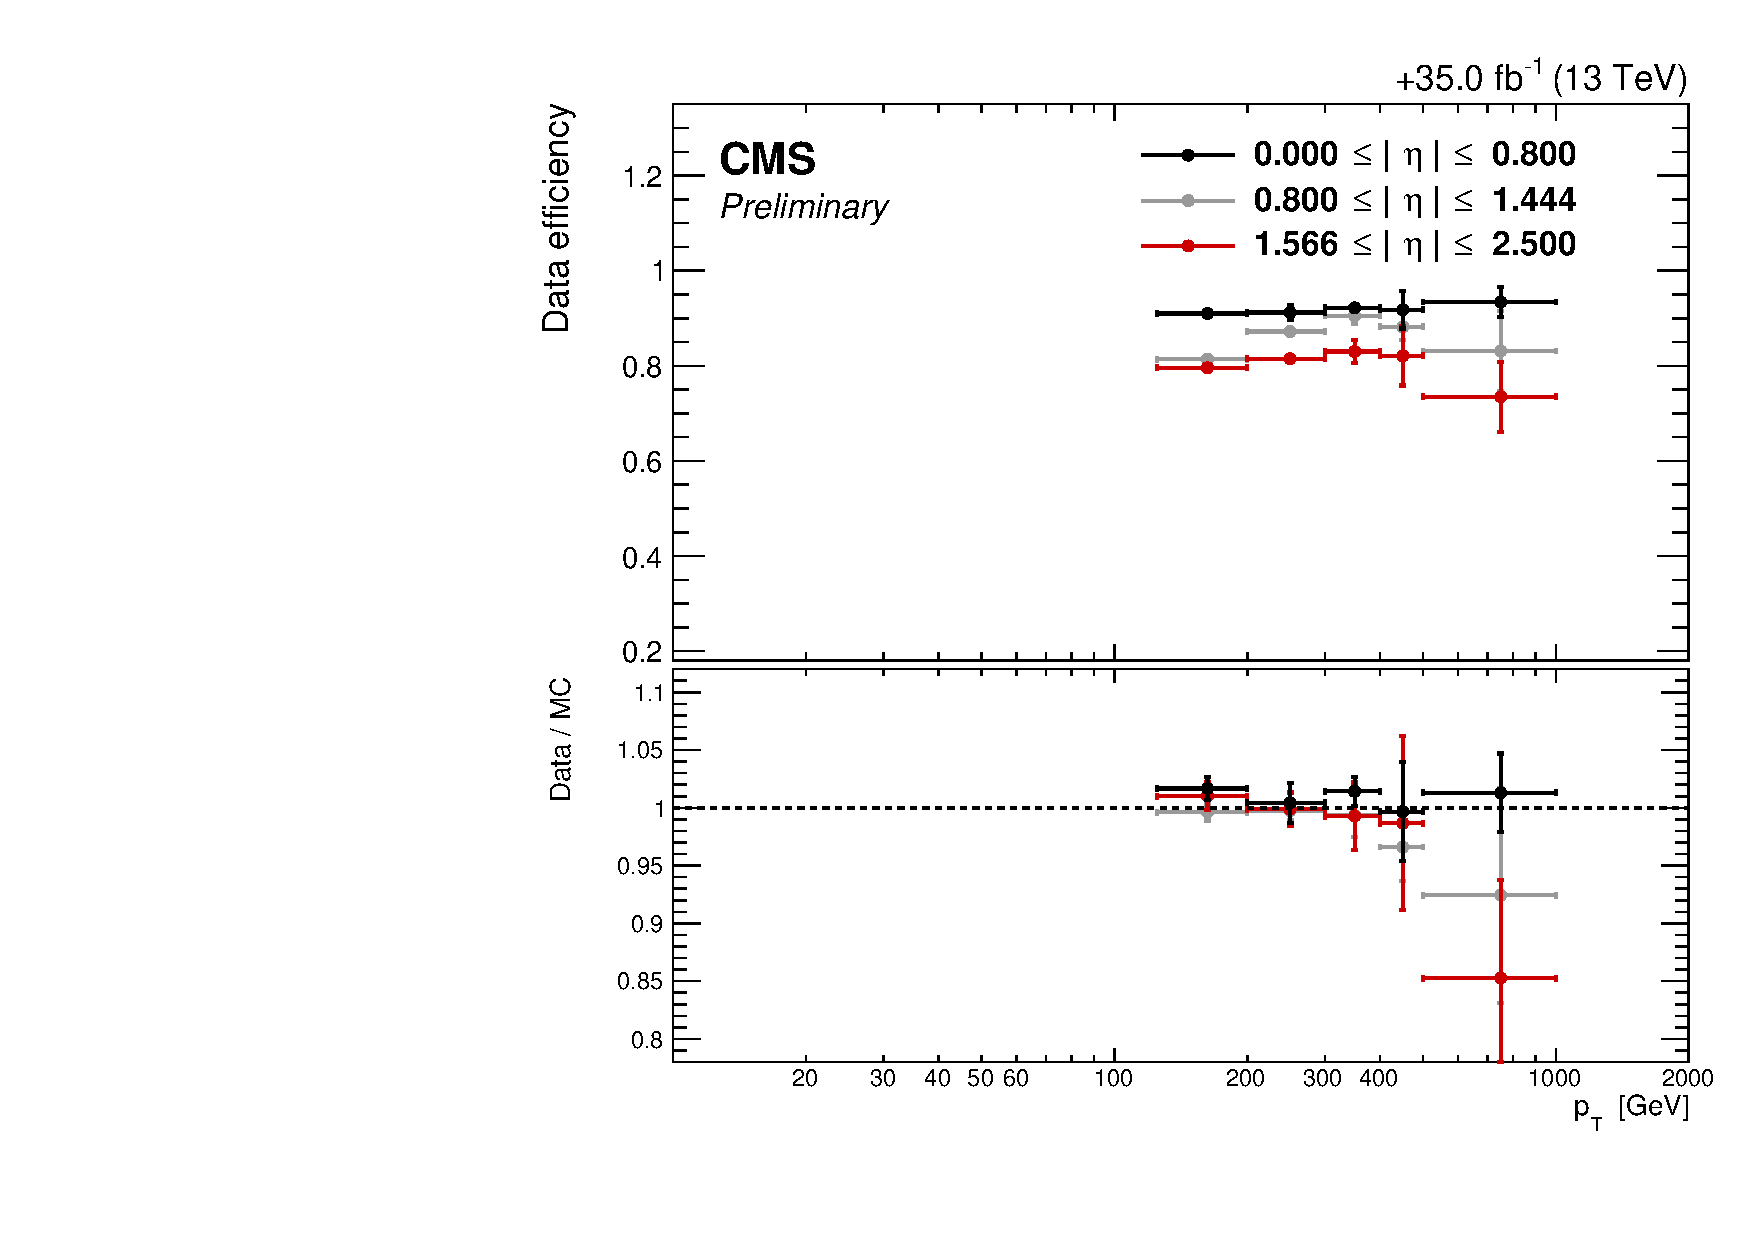
\includegraphics[angle=0,width=0.3\textwidth]{fig/eff2016.pdf}
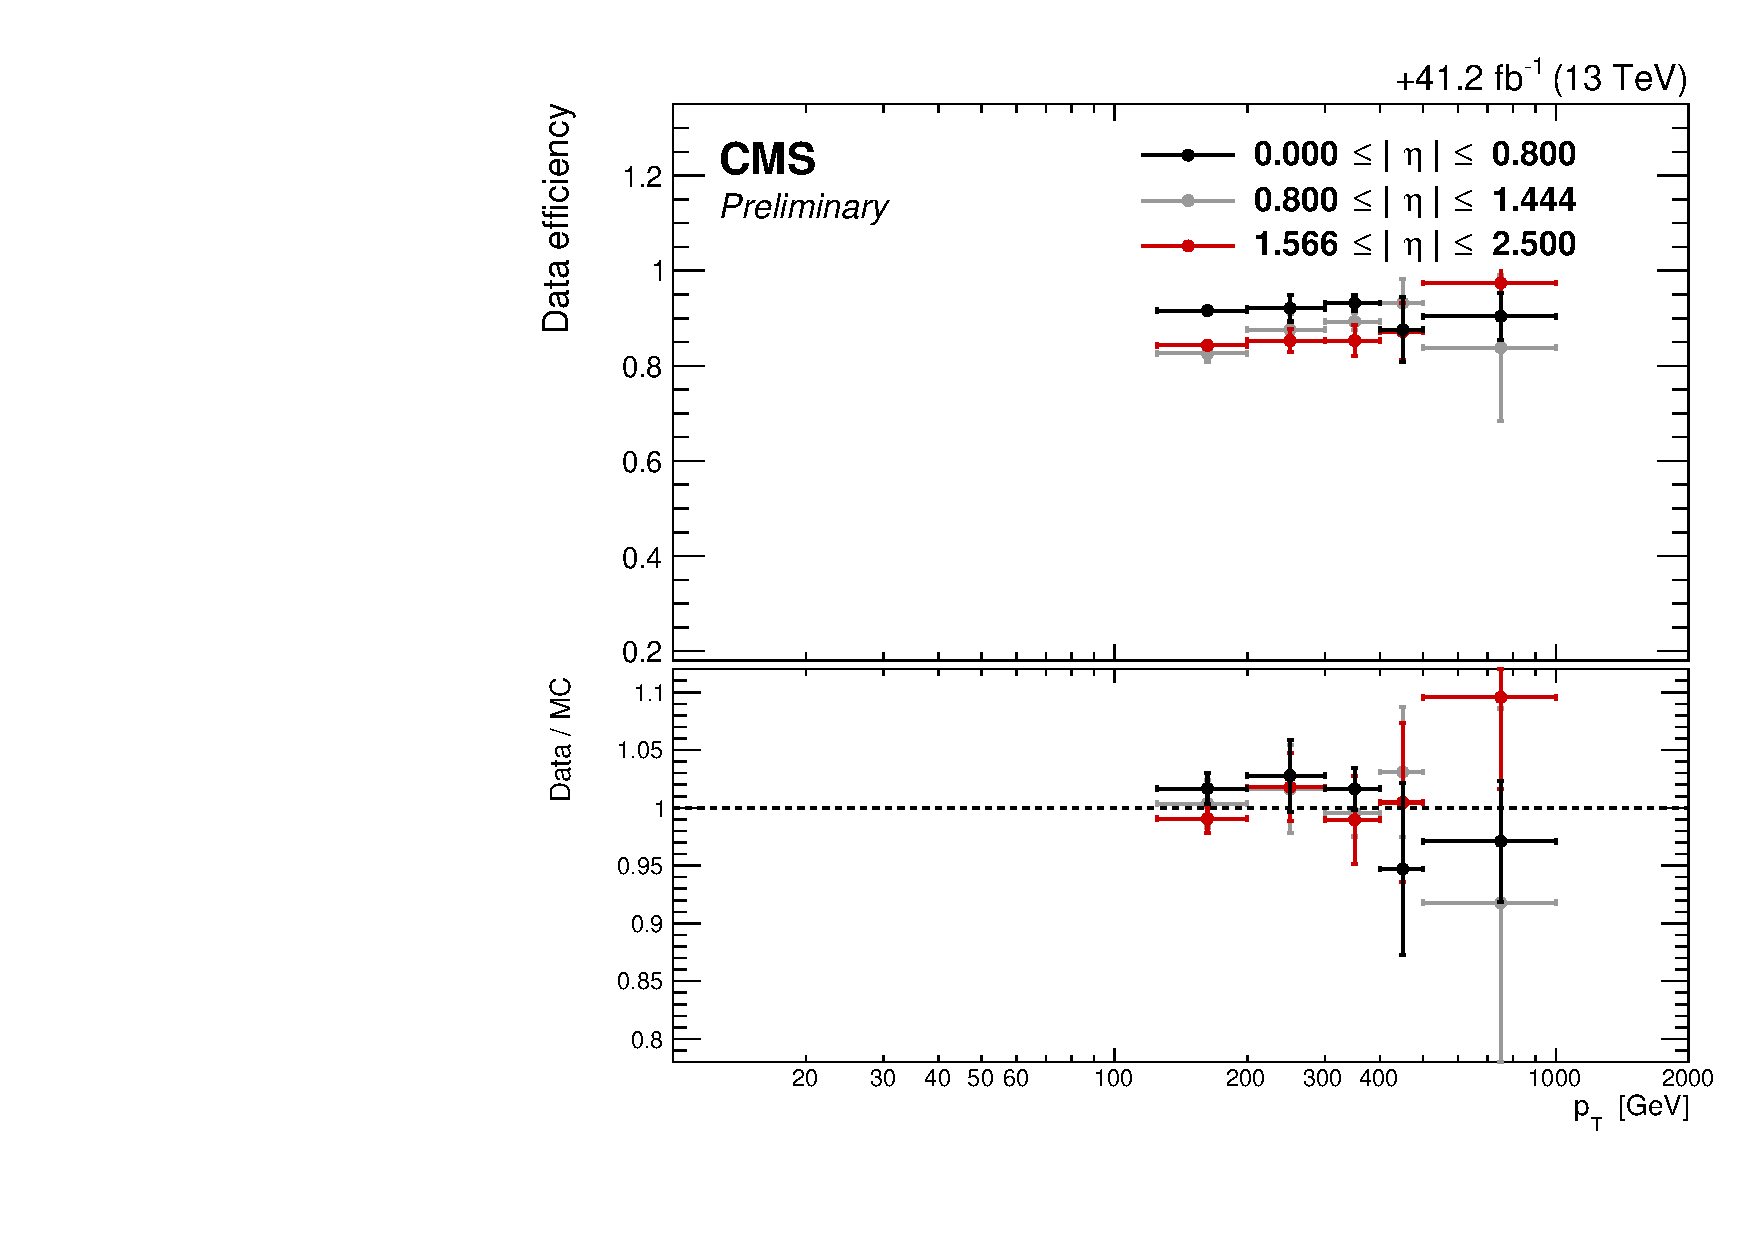
\includegraphics[angle=0,width=0.3\textwidth]{fig/eff2017.pdf}
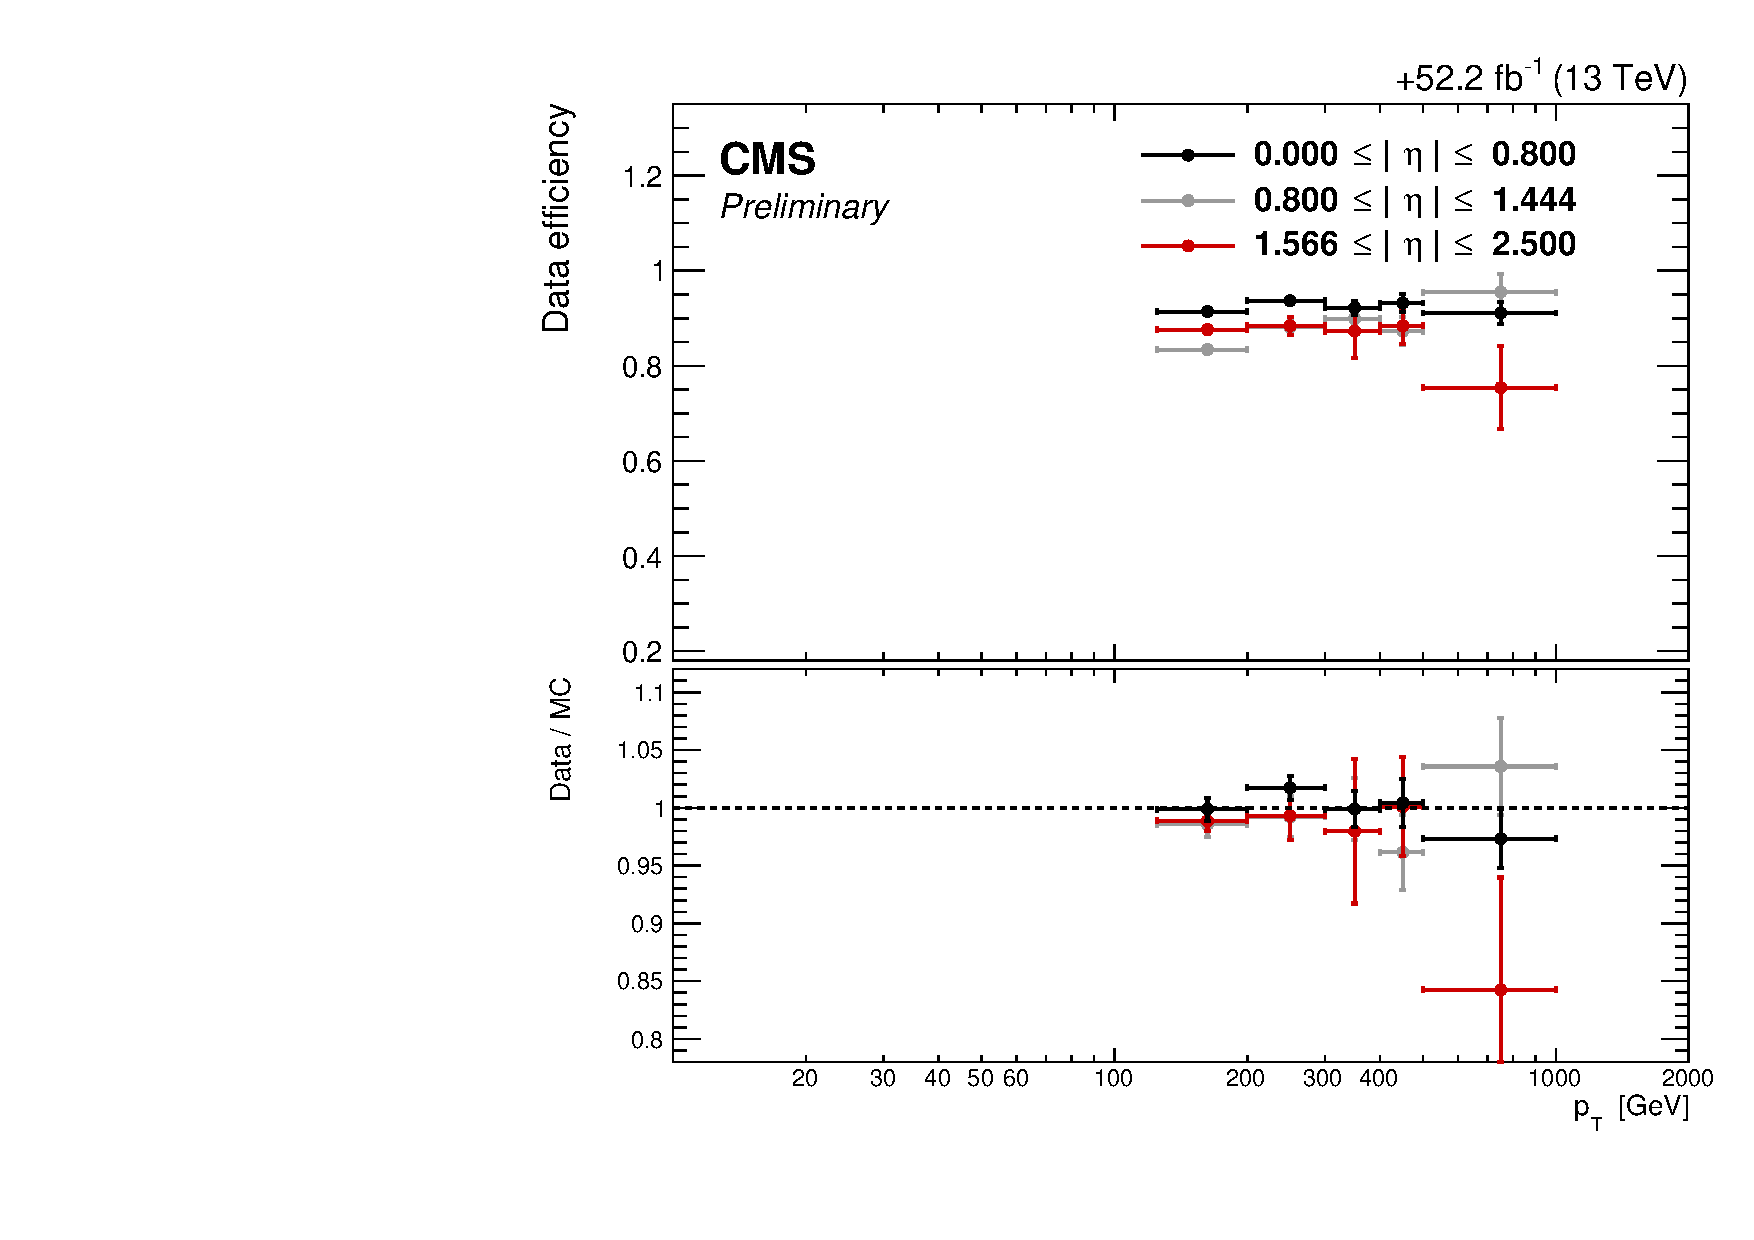
\includegraphics[angle=0,width=0.3\textwidth]{fig/eff2018.pdf}
\end{center}
~\label{fig:SFvsPt}
\end{figure}

% \begin{figure}[!htbp]
%   \centering
%   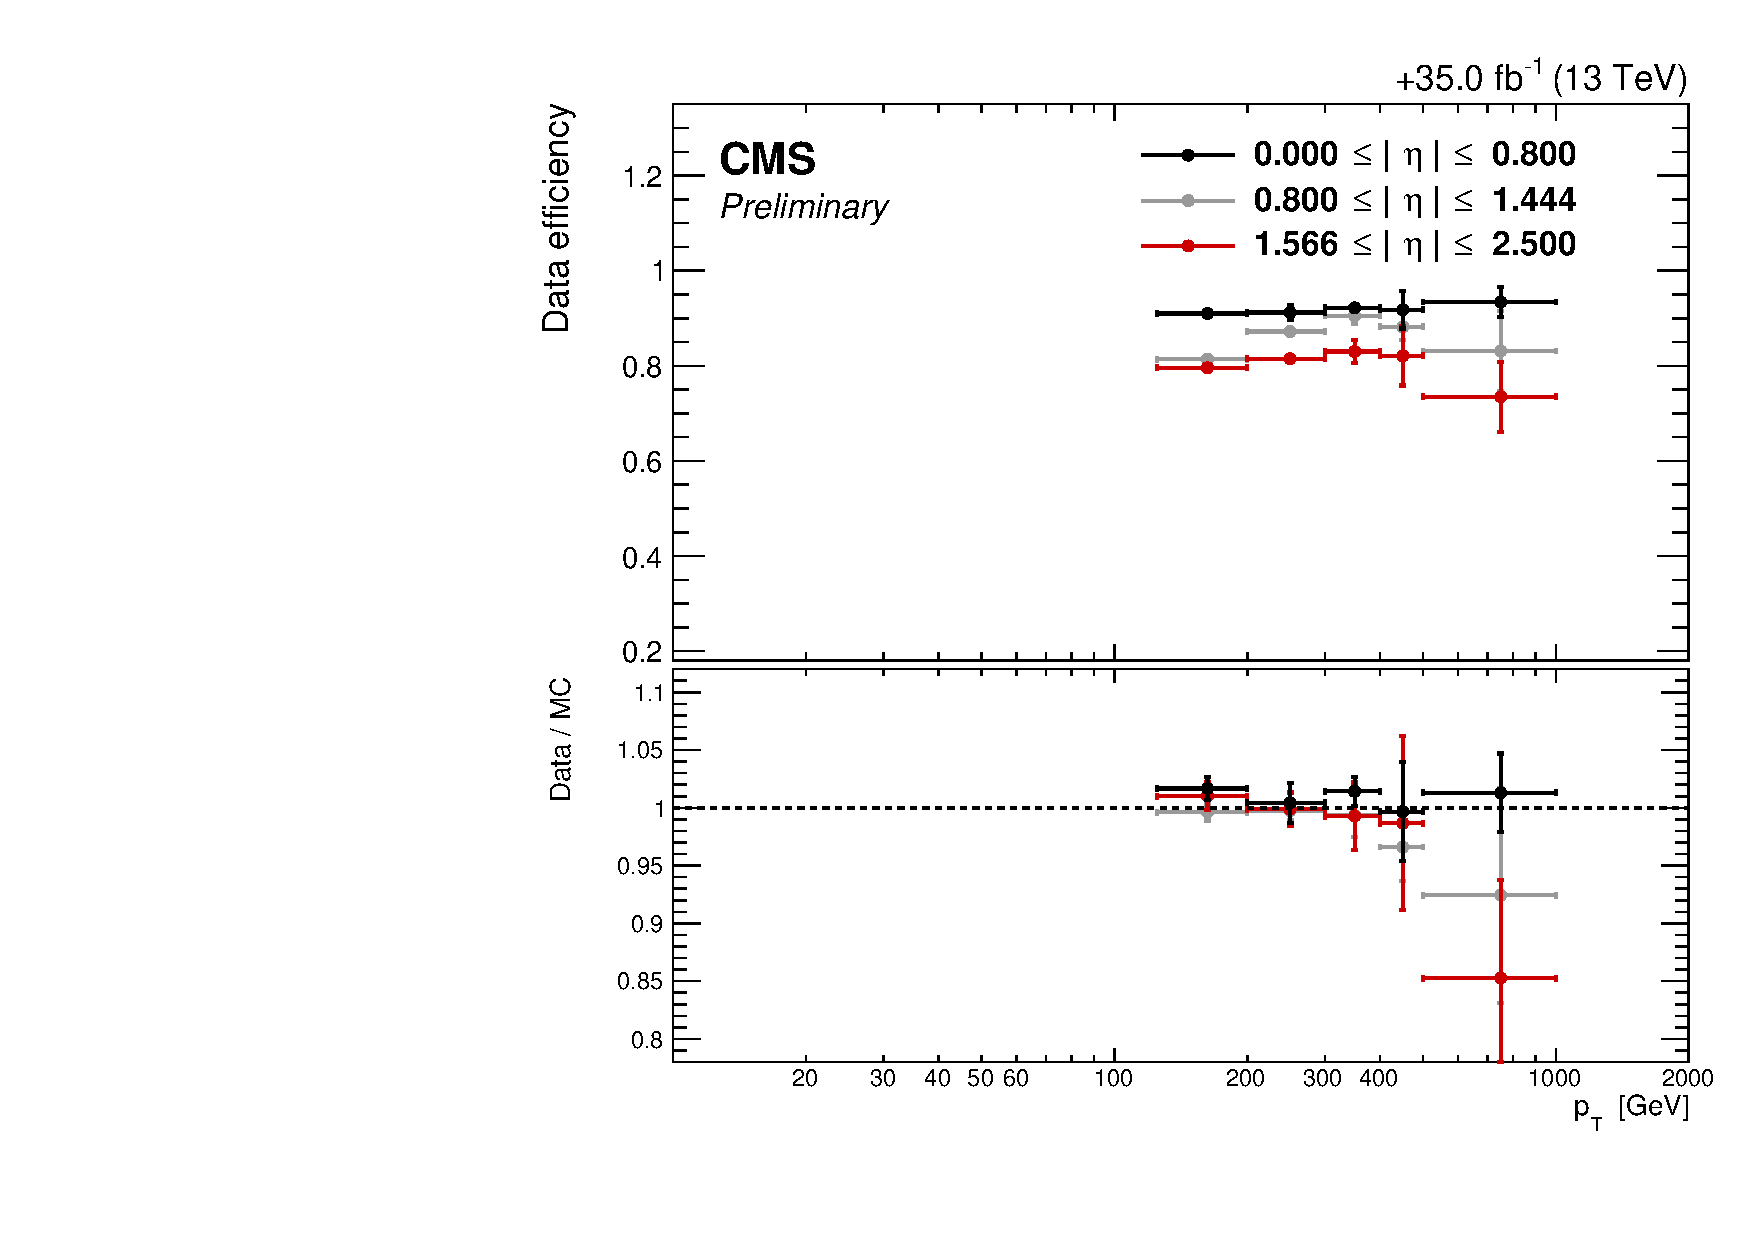
\includegraphics[width=0.3\textwidth]{fig/eff2016.pdf}\\
%   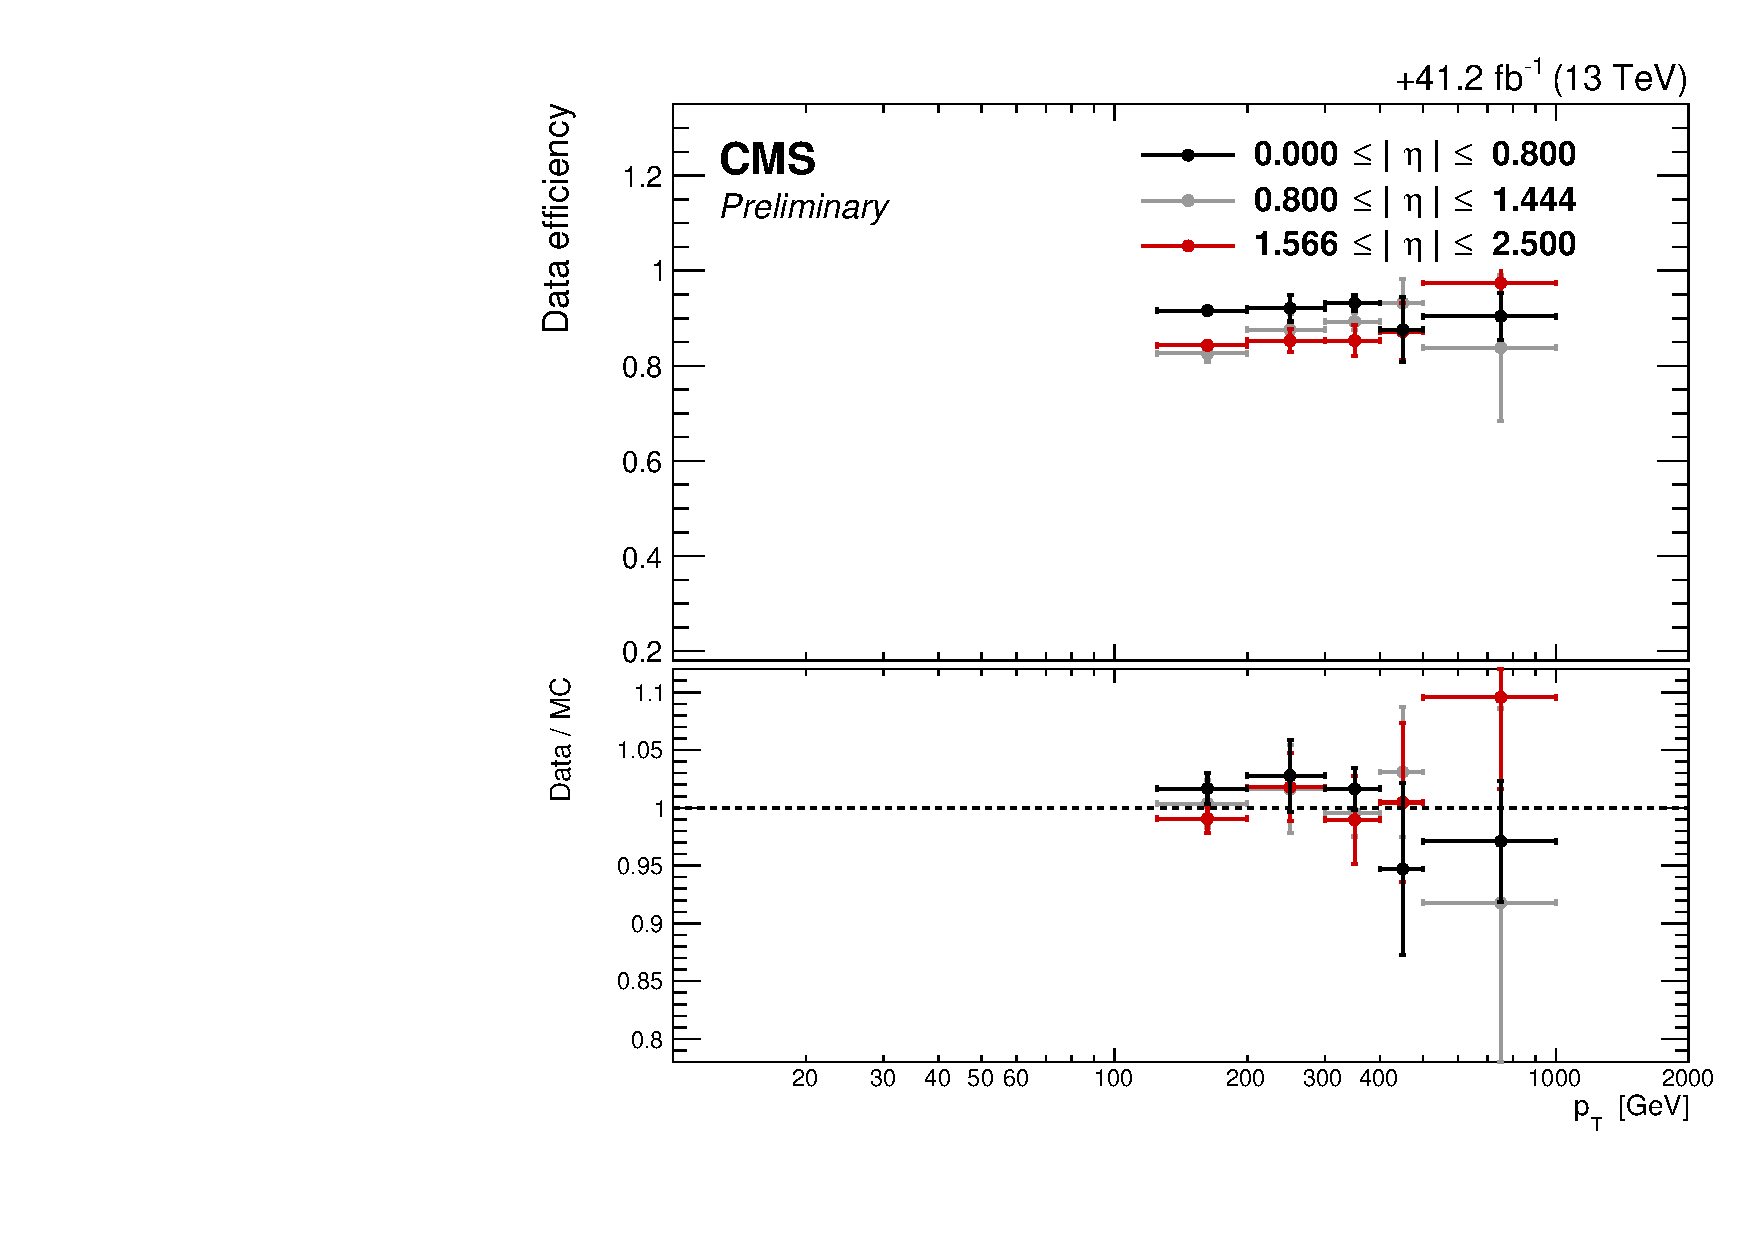
\includegraphics[width=0.3\textwidth]{fig/eff2017.pdf}\\
%   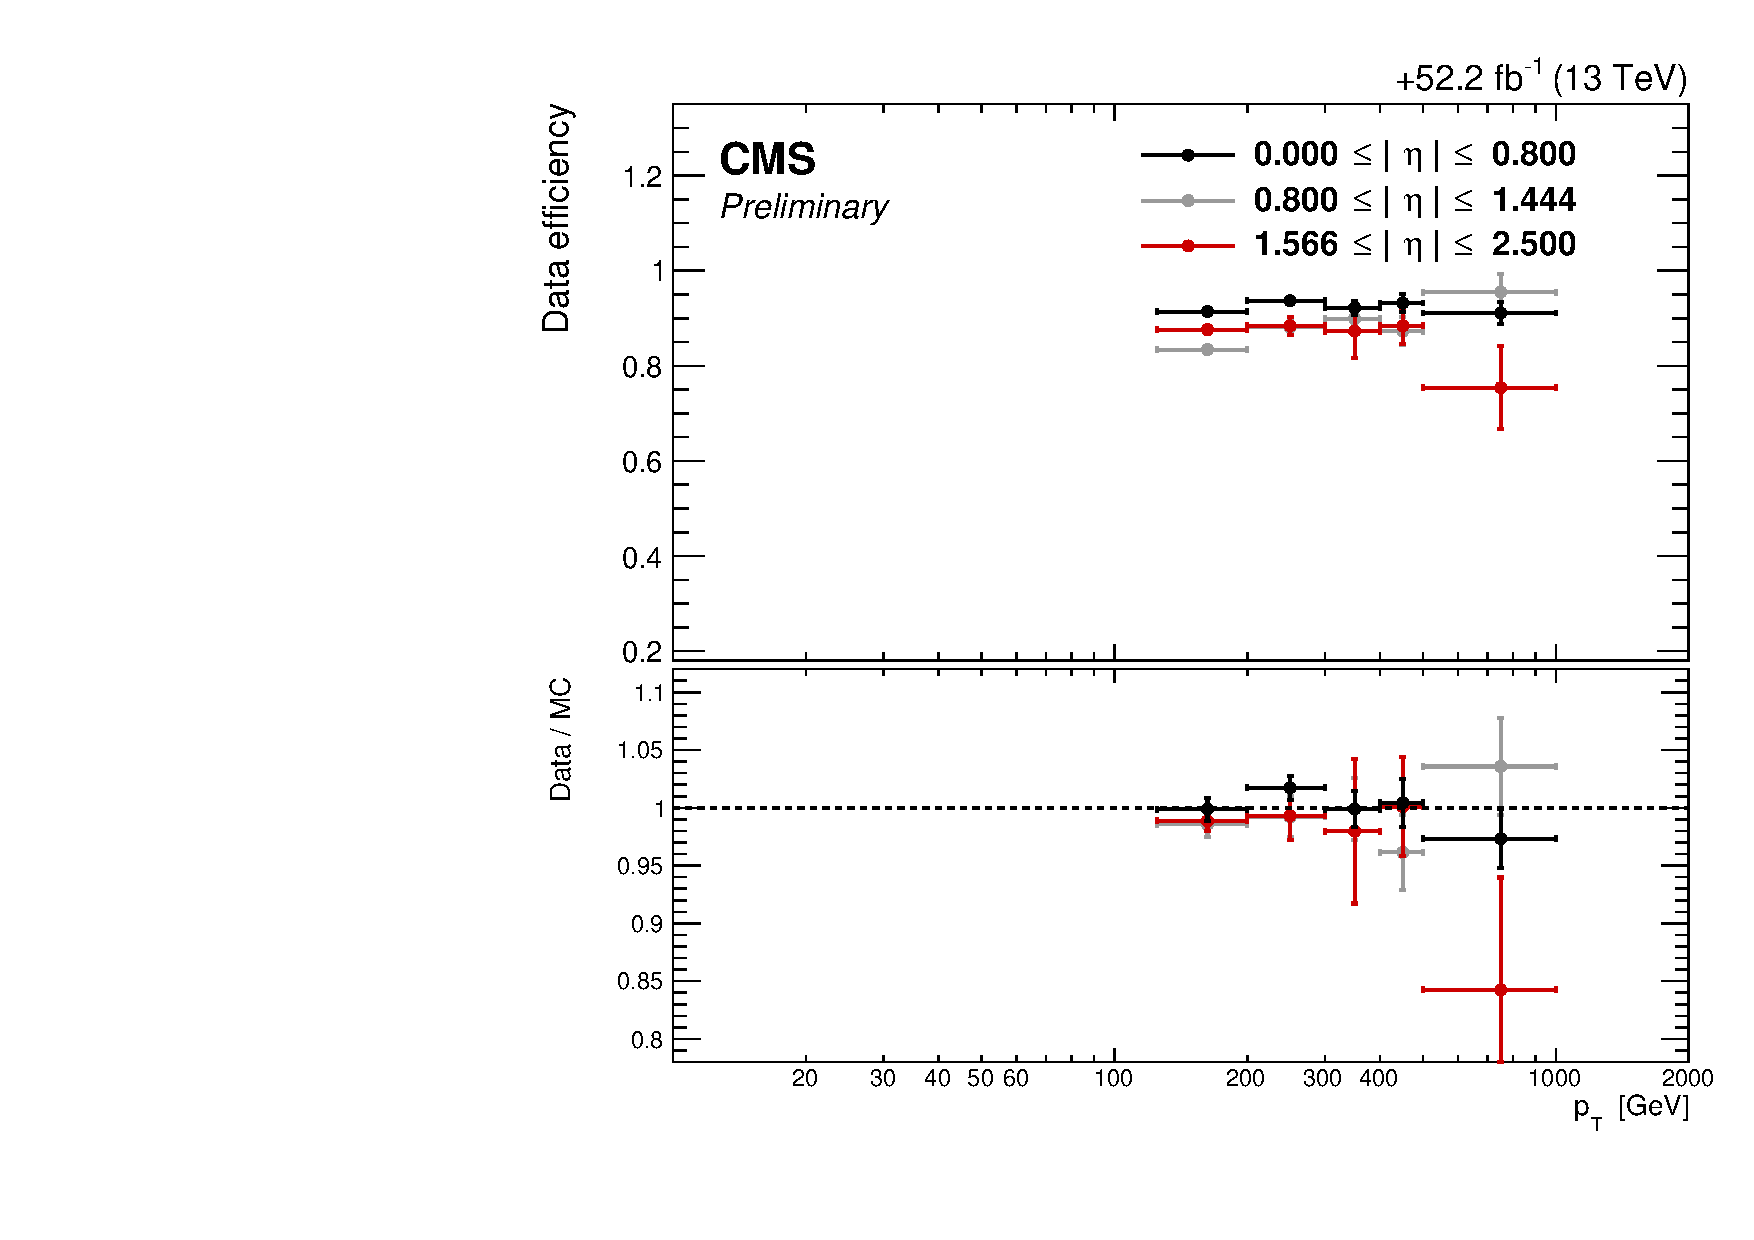
\includegraphics[width=0.3\textwidth]{fig/eff2018.pdf}}
%   \caption{}
%   \label{fig:SFvsPt}
% \end{figure}


\subsection{Datasets}~\label{sec:CMSDataRunII}~\label{sec:datasets}
In this analysis we used data collected by the CMS experiment from 2016 to the end of 2018, corresponding to a total integrated luminosity of 138~\fbinv. These samples are listed in Table~\ref{table:datasets2016-18}, fulfill the standard data quality criteria for all of the subdetectors of CMS as specified by the good run JSONs listed in Table~\ref{table:json}. These JSONs or JavaScript Object Notation are lightweight file formats which contains the details about specific run periods that are considered to be of high quality and good for analysis.


% The data samples considered for this analysis are listed in Table~\ref{table:datasets2016-18} and correspond to an integrated luminosity of 138~\fbinv collected by the CMS experiment from 2016 to the end of 2018. The 2016 and 2017 data sets were processed in {\tt CMSSW\_9\_4\_13}, while the 2018 data sets are processed using {\tt CMSSW\_10\_2\_16}. The global tags used to analyze the data are listed in Table~\ref{table:datasets2016-18}. These samples also fulfill standard data quality criteria for all the subdetectors of CMS as specified by the good run JSONs listed in Table~\ref{table:json}. 




% I don’t think you need the table of dataset names or JSOn names in your dissertation (unlike the internal AN). Nor CMSSW versions.  But do describe the lumi, the idea of applying data quality checks etc. Think about describing this to a non-CMS person – what is meaningful to them? (Its very different than CMS internal review)

\section{Endcap Region Issues}~\label{sec:EEIssues}
There were two known issues in the endcaps which had to be accounted for in CMS analyses. These issues were related to the L1 trigger prefiring~\cite{CMS:2020cmk, CMS_Collaboration_reweighting} and the HEM15/16 failures. We discuss the problem in more detail in this section and show that in both cases, the effects on this diphoton analysis were negligible. 

\subsection{EE L1 Prefiring}
From the end of the 2016 data taking and the beginning of Run 2, there was a slowly developing shift in the shape of the ECAL pulses. The effect showed as an increasing offset in the timing calibration of the pulses which resulted from a transparency loss of the ECAL crystals. It is assumed that this loss is radiation-induced as the endcap region is subject to higher fluxes of radiation compared to the ECAL barrel. The problem was realized in early 2018. For this reason, the trigger primitives of the L1 trigger located in the ECAL endcaps were not matched to the correct bunch crossing (BX). Since there is also a rule which prevents the L1 trigger to trigger on two consecutive bunch crossings, an event which should have been accepted by the L1 trigger could have been discarded inappropriately. To mitigate this issue a reweighting procedure was designed in Ref.~\cite{CMS_Collaboration_reweighting}.

The affected region of ECAL was in the pseudorapidity range $\eta >$ 2.5. Here the L1 trigger system “prefired” and accepted the earlier collision in BX-1, whereas BX 0 is the one of interest. This effect is not accounted for in Monte Carlo simulations. To mitigate the issue a weight is assigned to each object that can cause the prefire issue which are photons and jets. The weight is a probability for the object to cause the prefiring and the total weight assigned to the event is the probability that none of the objects causes a prefiring. We checked photons that land in the $2.25 < |\eta| <3.0$ affected region for both signal (Figure~\ref{fig:EEL1Prefiringcheck2} and background (Figure~\ref{fig:EEL1Prefiringcheck1}) Monte Carlo Events. The pre-firing has a 10\% effect on the samples but the overall effect on the analysis is less than 1\% as the endcap region only contributes 10\% additional sensitivity to the analysis. Since the combined EBEE region only constitutes 10\% of our sensitivity, and the issue is only present at the tail-end of 2016 and parts of 2017 data-taking, the overall effect is smaller than 1\%. Hence, no reweighting was necessary in accordance to the guidelines stipulated in Ref.~\cite{CMS_Collaboration_reweighting}.

\begin{figure}[!htbp]
	\centering
     \caption{Representative signal samples that land in the pseudorapidity range $2.25 < |\eta| <3.0$ which is affected by the prefiring.}
	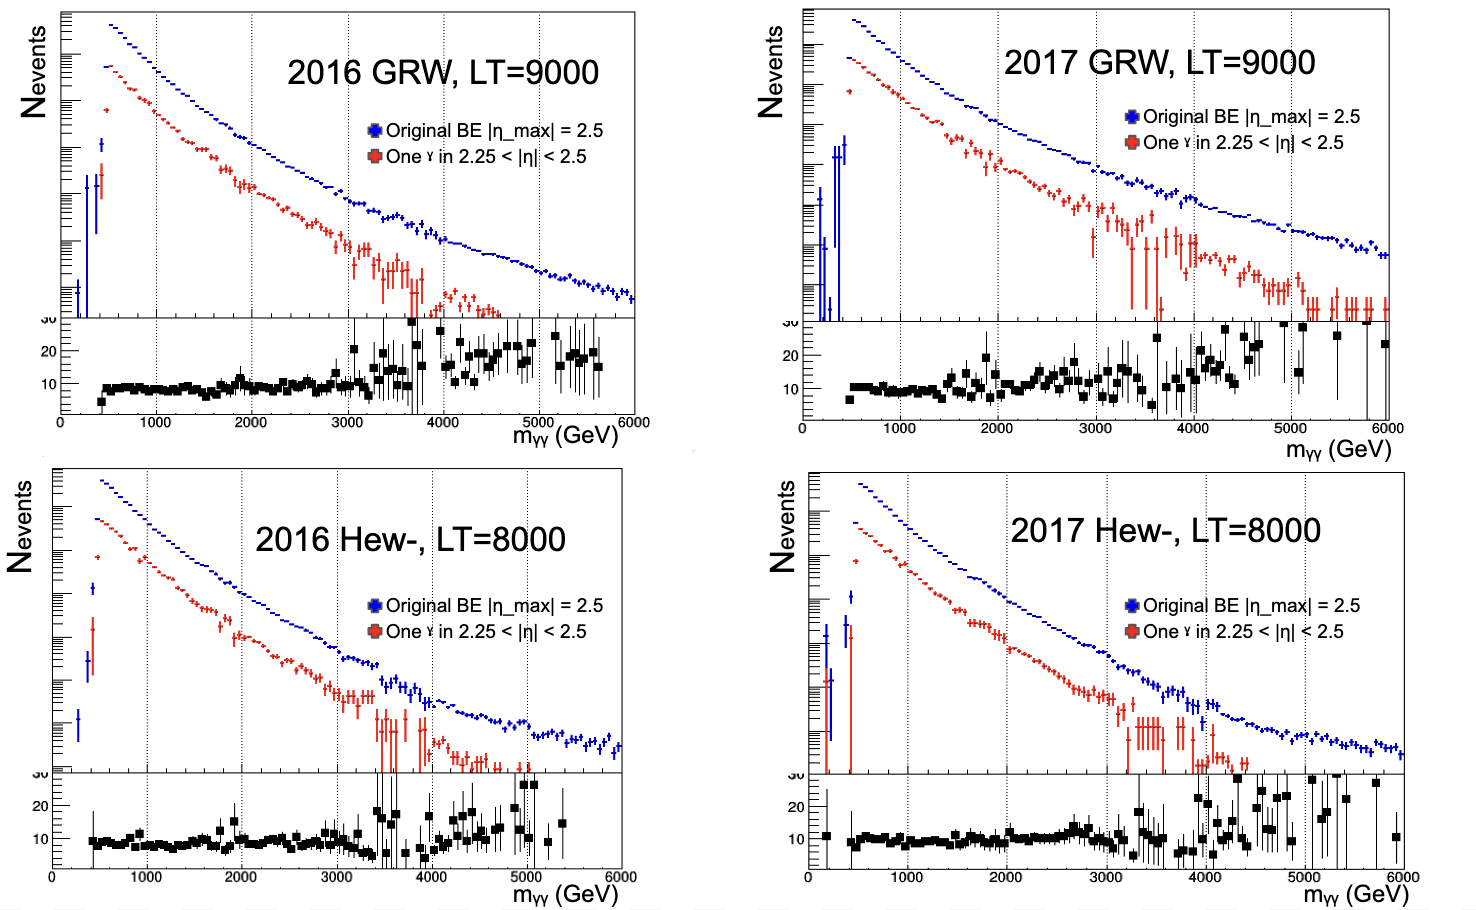
\includegraphics[scale=0.6]{fig/EEL1Prefiring2.png}
	\label{fig:EEL1Prefiringcheck2}
\end{figure}

% \begin{figure}[!htb]
% 	\centering
% 	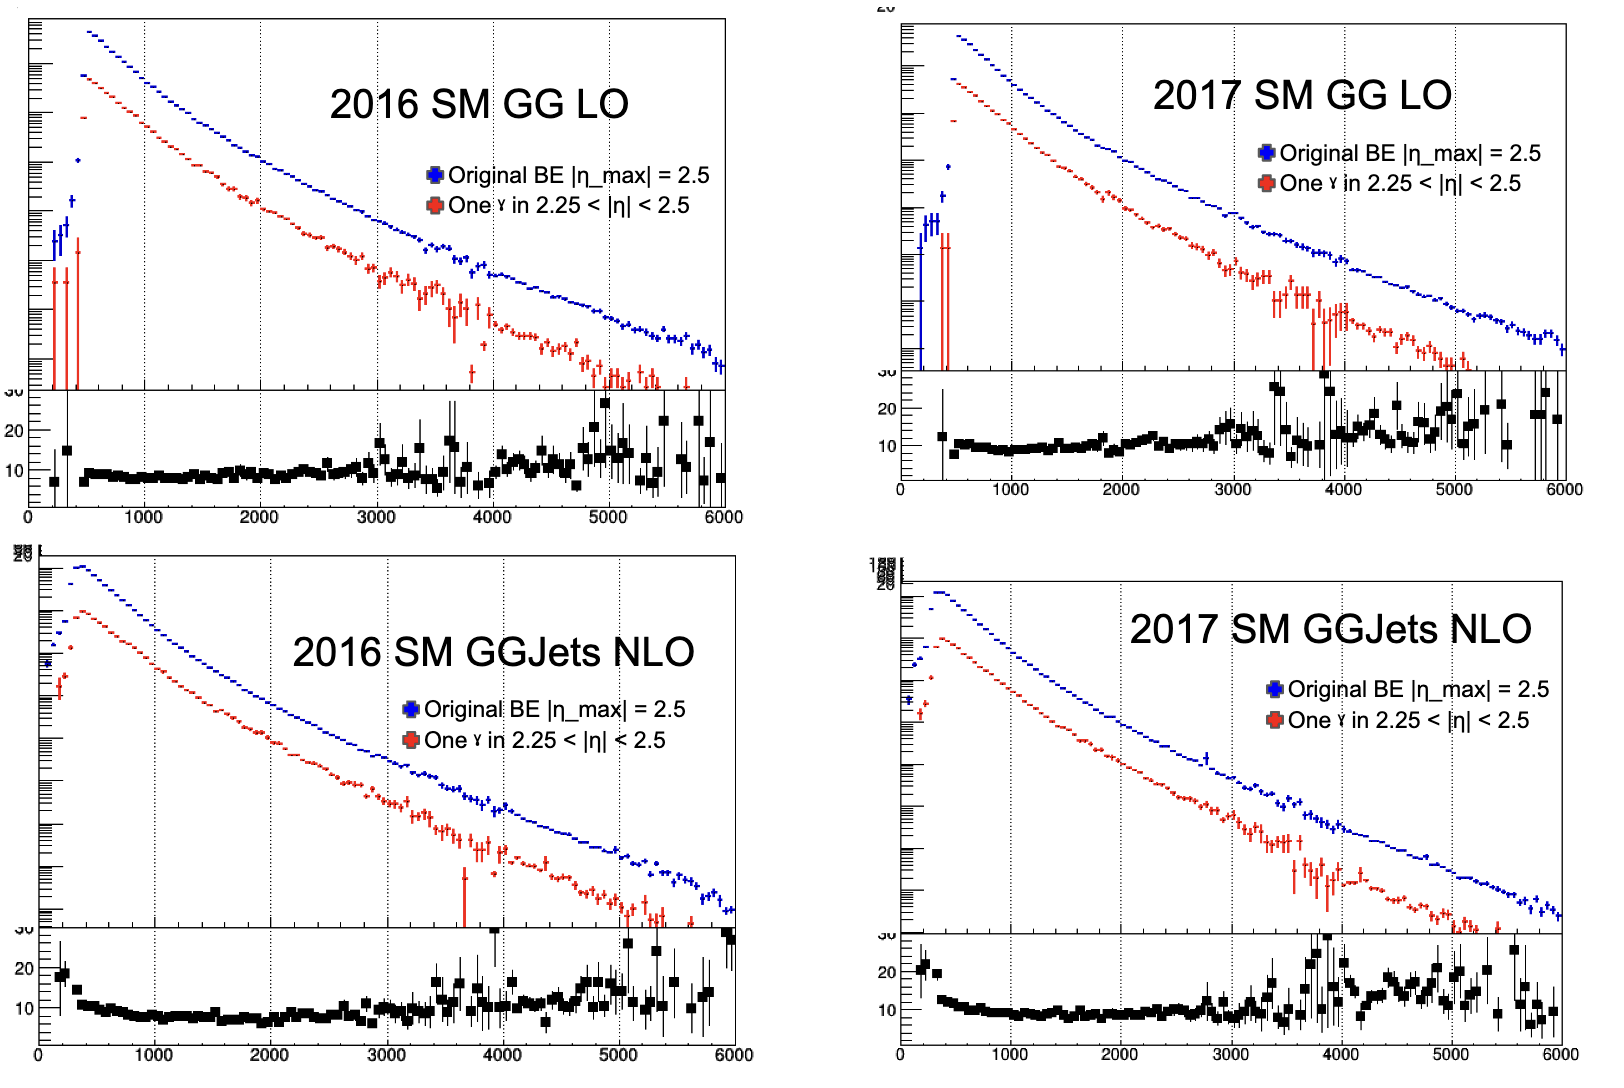
\includegraphics[scale=0.6]{fig/EEL1Prefiring1.png}
% 	\caption{Representative background samples that land in the pseudorapidity range $2.25 < |\eta| <3.0$ which is affected by the prefiring. The pre-firing has a 10\% effect on the samples but the overall effect on the analysis is less than 1\% as the endcap region only contributes 10\% additional sensitivity to the analysis.}
% 	\label{fig:EEL1Prefiringcheck1}
% \end{figure}

\begin{figure}[!htbp]
    \centering
      \caption{Representative background samples that land in the pseudorapidity range $2.25 < |\eta| < 3.0$, which is affected by the pre-firing.}
    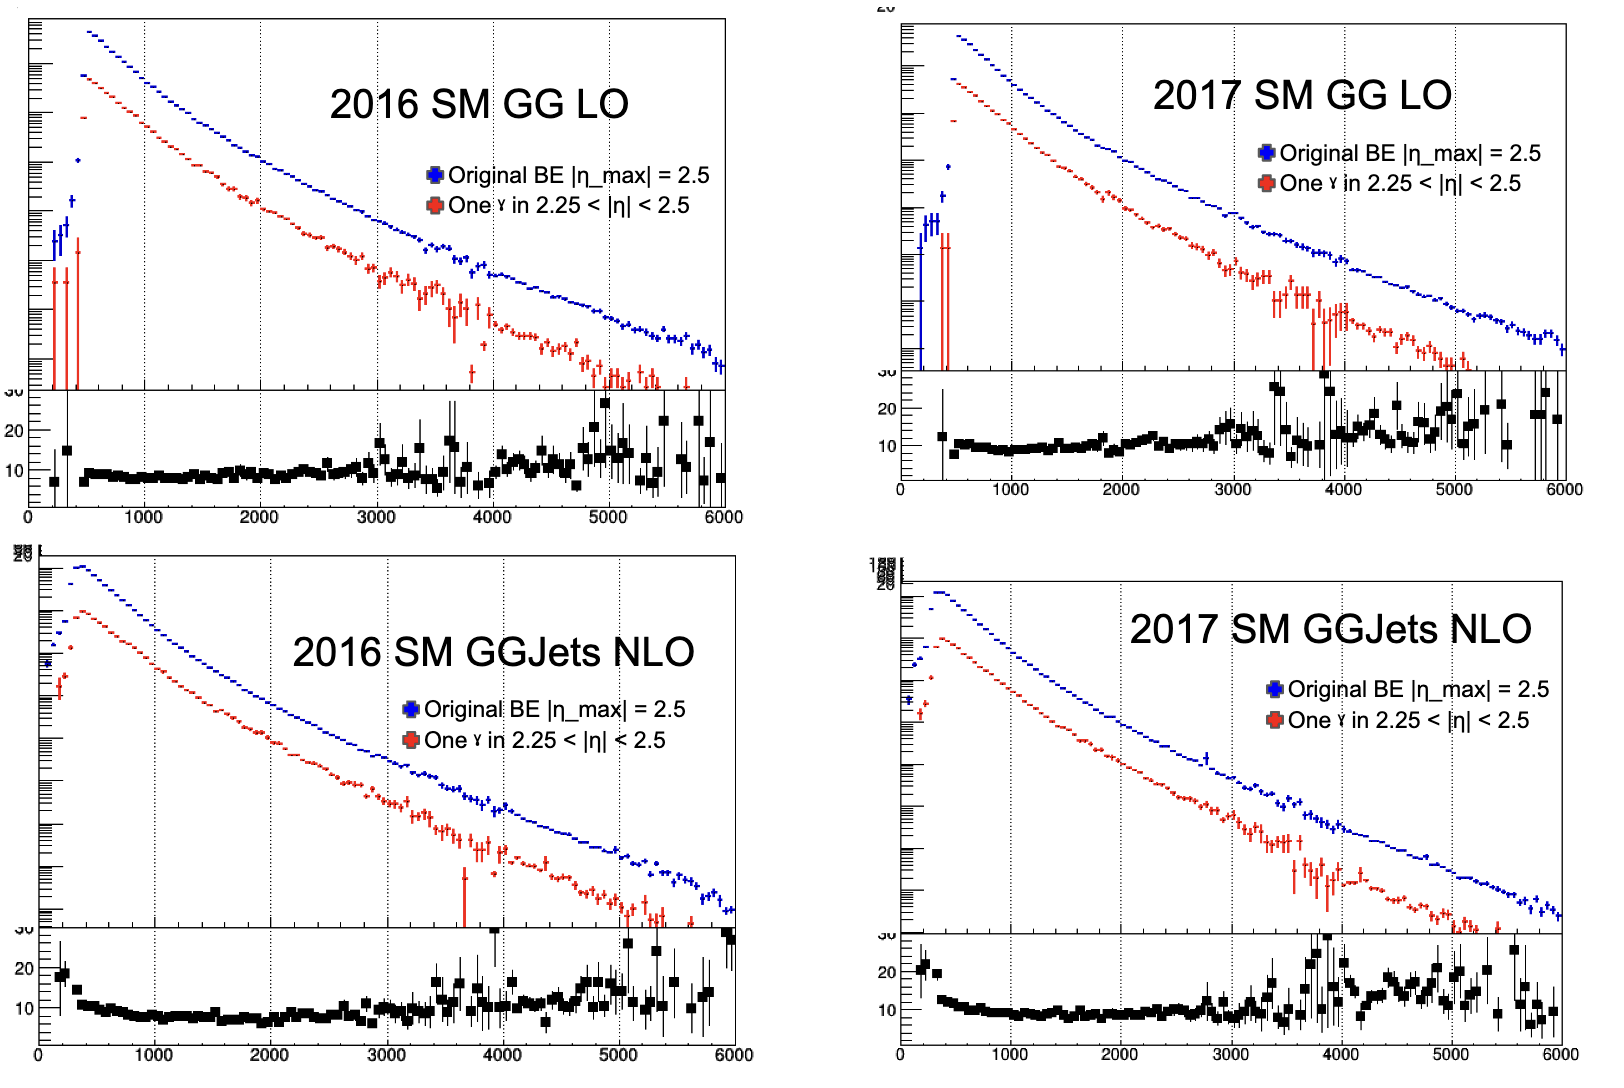
\includegraphics[scale=0.6]{fig/EEL1Prefiring1.png}
    \label{fig:EEL1Prefiringcheck1}
\end{figure}


\subsection{HEM 15/16: Endcap Minus Power Outage}

From May 2018 to December 2018, the HCAL endcap minus side experienced power issues in wedges 30-31 known as HEM15 an wedges 32-33 or HEM16 which is shown in the numbering scheme shown in Figure~\ref{fig:HCALwedges}. This issue then is isolated for run era C of the 2018 data taking. We compare in Figure~\ref{fig:HEM1516BarrelBeforeAndAfter} the diphoton mass spectrum in the control region before run A and B and after, run C and D the HEM15/16 issue. From the plots, we see no significant effects were seen. This is expected as HCAL is mostly seen as a veto for $e-\gamma$ events. 

\begin{figure}[!htbp]
	\centering
    \caption{Numbering scheme for the HCAL Wedges. Each wedge is 20 degrees.}
	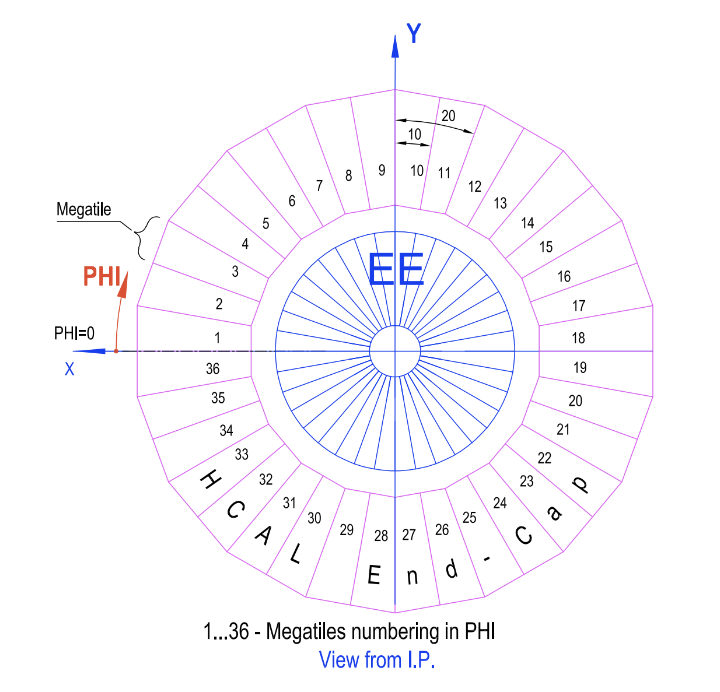
\includegraphics[scale=0.65]{fig/NumberingSchemeHCALWedges.png}
	\label{fig:HCALwedges}
\end{figure}


\begin{figure}[!htbp]
 \caption{No effects were seen on control region of the diphoton mass spectrum before and after the HEM15/16 issue.}
	\centering
   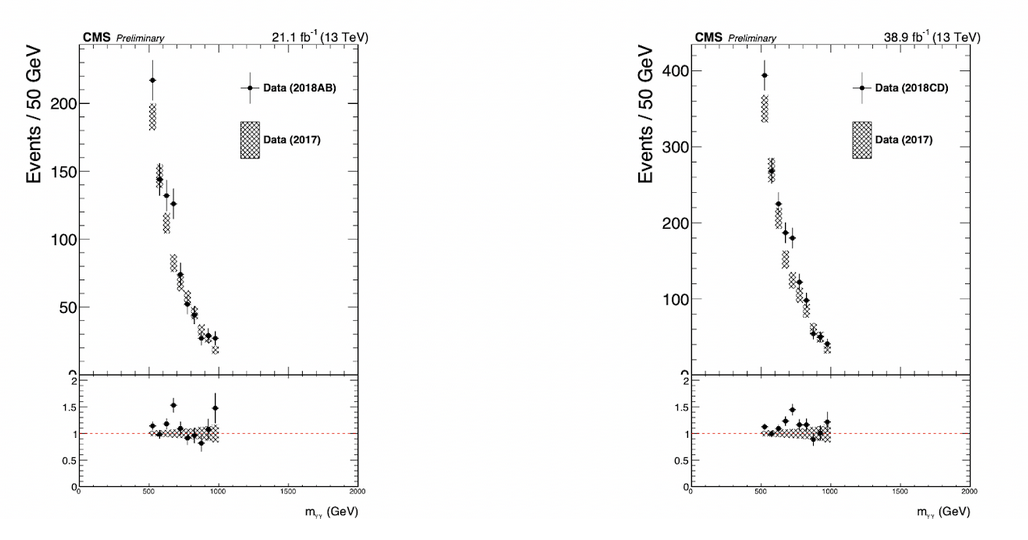
\includegraphics[scale=0.65]{fig/HEM15:16BarrelBeforeAndAfter.png}
	\label{fig:HEM1516BarrelBeforeAndAfter}
\end{figure}

% \begin{figure}[!htb]
% 	\centering
% 	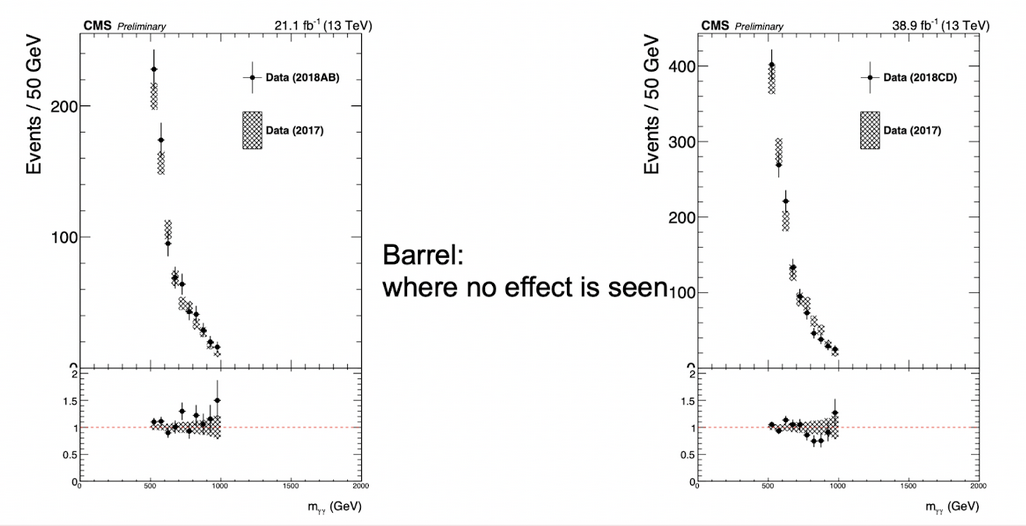
\includegraphics[scale=0.6]{fig/HEM15:16BarrellNoEff.png}
% 	\caption{No effects were seen on control region of the diphoton mass spectrum before and after the HEM15/16 issue.}
% 	\label{fig:HEM1516BarrelNoEff}
% \end{figure}


\newpage
% \section{References}
% \renewcommand{\bibsection}{}%removes the spaces and unwanted references heading from the list
% \begin{singlespacing}
% \bibliographystyle{apsrev}
% \bibliography{Ref_SignalSimClockwork.bib}
% \end{singlespacing}\par
% %{\let\thefootnote\relax\footnote{{Copyright: \copyright 2019 Elsevier B.V.}}}
